\section{Bayesian Estimation of Random Parameters}
\subsection{Introduction}
\begin{itemize}
    \item \textbf{Problem}: Derive an estimate of the value assumed by the random parameter \(Y\), which is not directly observable, given the observed data \(\{X_i\}\) that are related to \(Y\).
    \item From a mathematical point of view, the estimator is a function of the observed data vector \textbf{X} and it should provide a value that is the closest possibile to the true value assumed by the random parameter \(Y\) in that specific trial of the experiment under observation:
    \[
    \boxed{\mathbf{\hat{Y}=\hat{Y}(X)=\Phi(X_1,X_2,X_3,\cdots,X_N)}}
    \]
    \item Clearly, in order the observed data vector \textbf{X} to be useful for the estimation of the value assumed by \(Y\), there must be a relationship between them and this relationship should be known.
    \item In our problems this relationship is mathematically described by the pdf of \(Y\) conditioned to \textbf{X}(the \textit{a posteriori} pdf), or equivalently by the joint pdf of \(Y\) and \textbf{X}.
    \item \textbf{Bayesian approach}: the Bayes method to derive the estimator \(\Phi(\mathbf{x})\) consists on the definition of a cost function \(C\), which is a function of the estimation error \(\varepsilon\) and measures the cost of making an error, and then attempts to minimize the average cost \(R\), which is called \textbf{Bayes' Risk}:
\begin{align*}
R &\triangleq E_{Y,X}\!\left\{ C(\varepsilon) \right\}
   = E_{Y,X}\!\left\{ C\!\left(Y-\hat{Y}(\mathbf{X})\right) \right\} \\[4pt]
  &= \iint C\!\left(y-\hat{y}(\mathbf{x})\right)
          f_{Y,X}(y,\mathbf{x}) \, dy \, d\mathbf{x} \\[4pt]
  &= \iint \left[ \int_{-\infty}^{+\infty}
          C\!\left(y-\hat{y}(\mathbf{x})\right)
          f_{Y|X}(y \mid \mathbf{x}) \, dy \right]
          f_{X}(\mathbf{x}) \, d\mathbf{x} \\[4pt]
  &= E_{X}\!\left\{ E_{Y|X}\!\left[
          C\!\left(Y-\hat{Y}(\mathbf{X})\right)
        \right] \right\}.
\end{align*}

    \[
    \text{Since }f_X(\mathbf{x})\geq \quad\Rightarrow\quad\hat{Y}=\underset{\hat{y}}{\arg\min}=\underset{\hat{y}}{\arg\min } \hspace{4pt}E_{Y|\mathbf{X}}\{C(Y-\hat{Y}(\mathbf{X}))\}
    \]
    \item It is possible to define various cost functions; the most frequently used are the \textbf{quadratic cost function} and \textbf{uniform cost function}, which produce the \textbf{Minimum Mean Square Error (MMSE)} estimator and the \textbf{Maximum A Posteriori (MAP)} estimator, respectively.
    \item The \textbf{absolute value cost function} produces the \textbf{Median estimator}.
\begin{figure}[H]
    \centering
    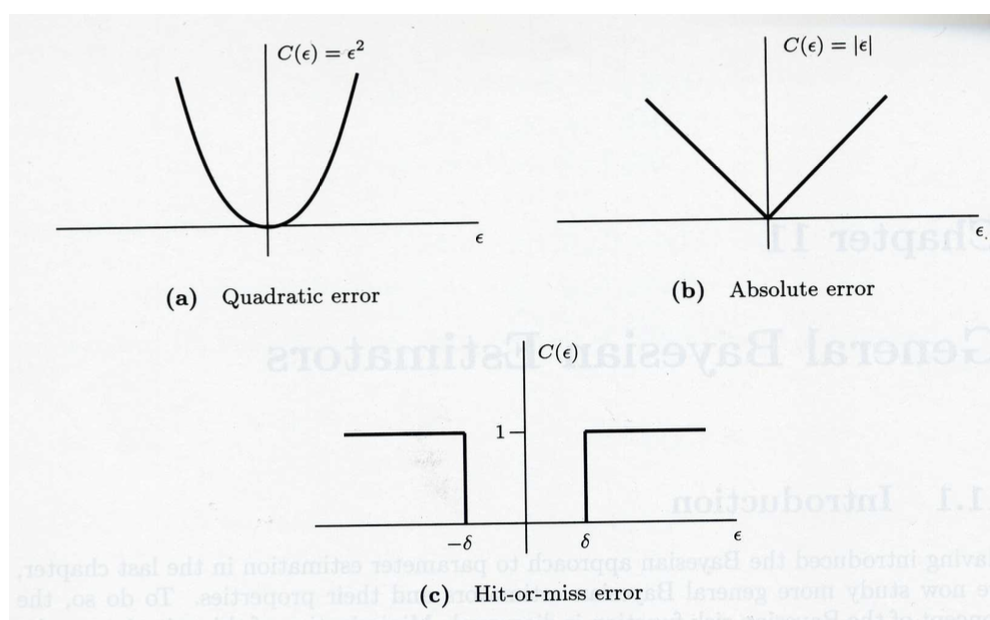
\includegraphics[width=0.65\linewidth]{Image/pdf 7/1.bo_1.png}
    \label{fig:placeholder}
\end{figure}
\item \textbf{Quadratic cost function}:
\[
C(\varepsilon)=|\varepsilon|^2\quad\Rightarrow\quad R=E\{|\varepsilon|^2\}=MSE
\]
\begin{align*}
\hat{Y}
&= \arg\min_{\hat{Y}} E_{Y|X}
   \Bigl\{ C\bigl( Y - \hat{Y}(\mathbf{X}) \bigr) \Bigr\}= \arg\min_{\hat{Y}} E_{Y|X}
   \Bigl\{ \bigl\lvert Y - \hat{Y}(\mathbf{X}) \bigr\rvert^{2} \Bigr\}.
\end{align*}

\item i.e. 
\begin{align*}
&\hat{Y}= \arg\min_{\hat{Y}} E_{Y|X}
   \Bigl\{ \bigl|Y - \hat{Y}(\mathbf{X})\bigr|^{2} \Bigr\}
   = \arg\min_{\hat{Y}}
   \left[ \int_{-\infty}^{+\infty}
      \bigl|y - \hat{Y}(\mathbf{x})\bigr|^{2}
      f_{Y|X}(y \mid \mathbf{x}) \, dy \right], \\[6pt]
&\frac{\partial}{\partial \hat{Y}(\mathbf{X})}
\left[ \int_{-\infty}^{+\infty}
   \bigl|y - \hat{Y}(\mathbf{x})\bigr|^{2}
   f_{Y|X}(y \mid \mathbf{x}) \, dy \right]
= -2 \int_{-\infty}^{+\infty}
   \bigl(y - \hat{Y}(\mathbf{x})\bigr)
   f_{Y|X}(y \mid \mathbf{x}) \, dy = 0 .
\end{align*}
\begin{align*}
\int_{-\infty}^{+\infty} \bigl(y - \hat{Y}(\mathbf{x})\bigr)
   f_{Y|X}(y \mid \mathbf{x}) \, dy &= 0
   \;\Rightarrow\;
   \int_{-\infty}^{+\infty} y f_{Y|X}(y \mid \mathbf{x}) \, dy
   = \int_{-\infty}^{+\infty} \hat{Y}(\mathbf{x})
     f_{Y|X}(y \mid \mathbf{x}) \, dy \\[4pt]
\Rightarrow\quad
\hat{Y}(\mathbf{x}) \int_{-\infty}^{+\infty} f_{Y|X}(y \mid \mathbf{x}) \, dy
&= \int_{-\infty}^{+\infty} y f_{Y|X}(y \mid \mathbf{x}) \, dy \\[4pt]
\Rightarrow\quad
\hat{Y}(\mathbf{x})
&= \int_{-\infty}^{+\infty} y f_{Y|X}(y \mid \mathbf{x}) \, dy
   = E\!\left\{ Y \mid \mathbf{X} = \mathbf{x} \right\}
   \equiv \hat{Y}_{\text{MMSE}} .
\end{align*}
\vspace{-1em}
\begin{align*}
R &= E_X \Bigl\{ E_{Y|X}
      \bigl\{ \lvert Y - \hat{Y}(\mathbf{X}) \rvert^{2} \bigr\} \Bigr\}
   = E_X \Bigl\{ E_{Y|X}
      \bigl\{ \lvert Y - E\{Y \mid \mathbf{X}\} \rvert^{2} \bigr\} \Bigr\} \\[4pt]
  &= E_X \Bigl\{ \operatorname{var}\{Y \mid \mathbf{X}\} \Bigr\}
   = \operatorname{MSE}\{\hat{Y}_{\text{MMSE}}\}.
\end{align*}
\item The MMSE estimator of \(Y\) given the data vector \textbf{X} is an \textbf{unbiased} estimator:

\begin{align*}
\hat{Y}_{\text{MMSE}}
&= E\{Y \mid \mathbf{X}\}
 = E_{Y|X}\{Y\}
 \equiv \eta_{Y|X}
 \qquad \text{(mean value of the a-posteriori pdf of } Y\text{)} \\[8pt]
E\{Y - \hat{Y}_{\text{MMSE}}\}
&= E_{Y,X}\{Y - \hat{Y}_{\text{MMSE}}\}
 = E_{Y,X}\{Y\} - E_{Y,X}\{\hat{Y}_{\text{MMSE}}\} \\[2pt]
&= E_Y\{Y\} - E_X\{ E_{Y|X}\{Y\} \}
 = \eta_Y - E_{Y,X}\{Y\}
 = \eta_Y - \eta_Y = 0
 \quad \Rightarrow \quad \text{unbiased}. \\[10pt]
\operatorname{MSE}\{\hat{Y}_{\text{MMSE}}\}
&= E\bigl\{(Y - \hat{Y}_{\text{MMSE}})^{2}\bigr\}
 = E\bigl\{(Y - E_{Y|X}\{Y\})^{2}\bigr\} \\[2pt]
&= E_{Y,X}\bigl\{(Y - \eta_{Y|X})^{2}\bigr\}
 = E_X\!\left\{ E_{Y|X}\bigl\{(Y - \eta_{Y|X})^{2}\bigr\} \right\} \\[2pt]
&= E_X\{\sigma_{Y|X}^{2}\}
 \quad \Rightarrow \quad \text{mean value of the conditional variance}.
\end{align*}

\item In summary, for the quadratic cost function we get: \(R=MSE\) and 
\begin{align*}
&\hat{Y}_{\text{MMSE}}
= E\{Y \mid \mathbf{X}\}
 = \int_{-\infty}^{+\infty}
   y \, f_{Y|X}(y \mid \mathbf{x}) \, dy
 \qquad \text{mean value of the a-posteriori pdf}, \\[6pt]
&\operatorname{MSE}\{\hat{Y}_{\text{MMSE}}\}
= E_X\!\left\{ \operatorname{var}\{Y \mid \mathbf{X}\} \right\}
 \qquad \text{mean value w.r.t. } \mathbf{x} \text{ of the conditional variance}.
\end{align*}

\item Hence, to derive the \textbf{MMSE estimator} of the random parameter \(Y\) given the observed adta vector \textbf{X}, we should derive its (conditional) mean and variance. These quantities provide the MMSE estimator and its MSE, respectively (after averaging w.r.t \textbf{X}).
\item The \textbf{a-posteriori pdf} describes the statistical behavior of \(Y\) after we have observed \textbf{X}. Before the observation of \textbf{X}, the statistical model of \(Y\) is provided by its a-priori pdf \(f_Y(y)\).
\[
C(\varepsilon)=1-\text{rect}\left(\frac{\varepsilon}{2\delta}\right)=
\begin{cases}
    0 &|\varepsilon|\leq\delta \\[4pt]
    1 &|\varepsilon|>\delta
\end{cases}
\]
\item We should solve the minimization problem:
\[
\hat{Y}=\underset{\hat{y}}{\arg\min}E_{Y|\mathbf{X}}\{C(Y-\hat{Y}(\mathbf{X})\}
\]
\item Where:
\begin{align*}
E_{Y|X}\!\left\{ C\bigl(Y - \hat{Y}(\mathbf{X})\bigr) \right\}
&= \int_{-\infty}^{+\infty}
   C\bigl(y - \hat{y}(\mathbf{x})\bigr) \,
   f_{Y|X}(y \mid \mathbf{x}) \, dy \\[4pt]
&= \int_{-\infty}^{+\infty}
   \left[ 1 - \operatorname{rect}
      \!\left(\frac{y - \hat{y}(\mathbf{x})}{2\delta}\right) \right]
   f_{Y|X}(y \mid \mathbf{x}) \, dy \\[4pt]
&= \int_{-\infty}^{+\infty}
   f_{Y|X}(y \mid \mathbf{x}) \, dy
   - \int_{-\infty}^{+\infty}
     \operatorname{rect}\!\left(\frac{y - \hat{y}(\mathbf{x})}{2\delta}\right)
     f_{Y|X}(y \mid \mathbf{x}) \, dy \\[4pt]
&= 1 - \int_{\hat{y}-\delta}^{\hat{y}+\delta}
        f_{Y|X}(y \mid \mathbf{x}) \, dy .
\end{align*}
\begin{align*}\hspace{-2em}
\hat{Y}
&= \arg\min_{\hat{y}} E_{Y|X}\!\left\{
   C\bigl(Y - \hat{Y}(\mathbf{X})\bigr) \right\} = \arg\min_{\hat{y}}
   \left[ 1 - \int_{\hat{y}-\delta}^{\hat{y}+\delta}
      f_{Y|X}(y \mid \mathbf{x}) \, dy \right] = \arg\max_{\hat{y}}
   \left[ \int_{\hat{y}-\delta}^{\hat{y}+\delta}
      f_{Y|X}(y \mid \mathbf{x}) \, dy \right].
\end{align*}


\item If \(\delta\) is small, the a-posteriori pdf can be assumed constant over the interval of size \(2\delta\), so that:
\begin{align*}
\hat{Y}_{\text{MAP}}
&= \arg\max_{y} f_{Y|X}(y \mid \mathbf{x})
 = \arg\max_{y} \frac{f_{Y,X}(y,\mathbf{x})}{f_X(\mathbf{x})}
 = \arg\max_{y} \frac{f_{X|Y}(\mathbf{x} \mid y) f_Y(y)}{f_X(\mathbf{x})} \\[4pt]
&= \arg\max_{y} f_{X|Y}(\mathbf{x} \mid y) f_Y(y)
 = \arg\max_{y} LF(y)\, f_Y(y),
\end{align*}
\[
\text{where} \quad
f_X(\mathbf{x}) = \int f_{Y,X}(y,\mathbf{x}) \, dy
 = \int f_{X|Y}(\mathbf{x} \mid y) f_Y(y) \, dy .
\]

\begin{align*}
\hat{Y}
&= \arg\max_{\hat{y}}
   \left[ \int_{\hat{y}-\delta}^{\hat{y}+\delta}
      f_{Y|X}(y \mid \mathbf{x}) \, dy \right]
 = \arg\max_{\hat{y}}
   \left[ f_{Y|X}(\hat{y} \mid \mathbf{x}) \cdot 2\delta \right]= \arg\max_{y} f_{Y|X}(y \mid \mathbf{x}) .
\end{align*}
\item In summary, if we adopt the "hit-or-miss" cost function, the estimator is given by the \textbf{mode} of the a-posteriori pdf and it is called the \textbf{Maximum A posteriori (MAP)} estimator:
\[
\hat{Y}_{MAP}=\underset{y}{\arg\max}f_{Y|\mathbf{X}}(y|\mathbf{x})
\]
\item Note that to maximize the a-posteriori pdf is equivalent to maximize the joint pdf of \(Y\) and \textbf{X}, since the denominator \(f_{\mathbf{X}}(\mathbf{x})\) does not depend on \(y\):
\item \textbf{Example}: derive the MAP estimator of a constant random signal \(A\) based on the observation of the \(N\) samples \(X_i=A+W_i\), where the noise samples \(W_i\) are IID, zero mean and Gaussian, and knowing that \(A\) is uniformly distributed between \(-A_0\) and \(A_0\):
\[
\hat{A}_{MAP}=\underset{a}{\arg\max}f_{\mathbf{X}|A}(\mathbf{x|a})f_A(a)
\]
\begin{figure}[H]
    \centering
    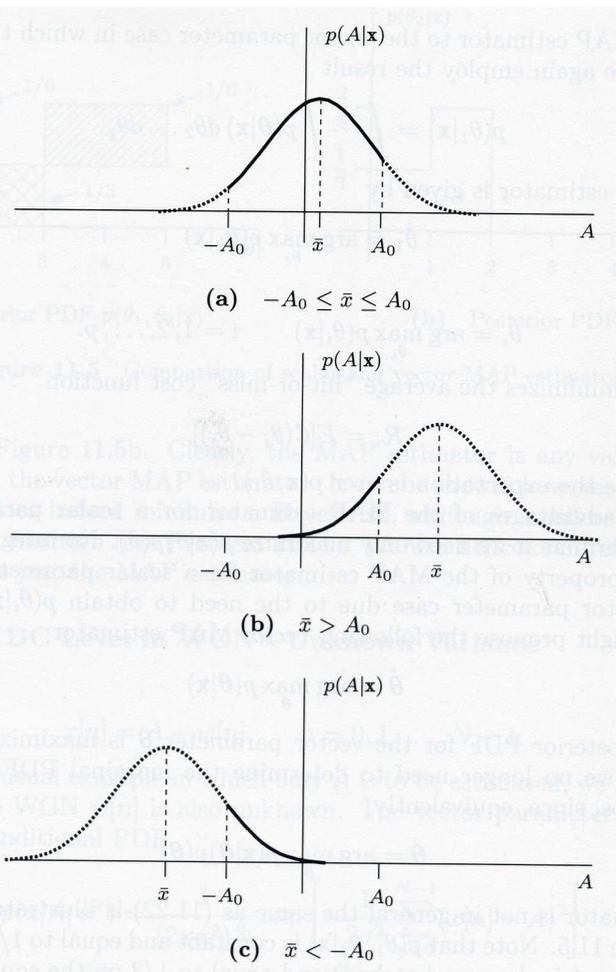
\includegraphics[width=0.3\linewidth]{Image/pdf 7/2.MAP.png}
    \label{fig:placeholder}
\end{figure}
\item As we already know, the maximum of teh pdf of \textbf{X} conditioned to \(A\) is given by the sample mean of the data (which is also the ML estimate of \(A\)). The a-priori pdf of \(A\) relocates the position of the maximum, favouring those values of \(A\) that are more likely to be obeserved.
\item Moreover, to maximize the joint pdf is equivalent to maximize its logarithm (or any monotonic increasing function of it):
\begin{align*}
\hat{Y}_{\text{MAP}}
&= \arg\max_{y} \ln f_{Y,X}(y,\mathbf{x})
 = \arg\max_{y} \ln\!\bigl[ f_{X|Y}(\mathbf{x} \mid y) f_Y(y) \bigr] \\[4pt]
&= \arg\max_{y} \Bigl[ \ln f_{X|Y}(\mathbf{x} \mid y)
                     + \ln f_Y(y) \Bigr].
\end{align*}
\item Hence, so as for the ML estimate, also the MAP estimate can be derived by differentiating (if the function is differentiable) the log of the joint pdf and solving the equation that we get by setting the derivative equal to zero (it is the so-called \textbf{MAP equation}):
\begin{align*}
\frac{\partial}{\partial y}
\Bigl[ f_{X|Y}(\mathbf{x} \mid y)\, f_Y(y) \Bigr] &= 0,
\qquad\text{or}\qquad
\frac{\partial}{\partial y}
\Bigl[ \ln f_{X|Y}(\mathbf{x} \mid y) + \ln f_Y(y) \Bigr] = 0 .
\end{align*}
\item In the case we adopt the \textbf{absolute cost function}, \(C(\varepsilon)=|\varepsilon|\), we obtain that the optimal estimate is given by the \textbf{median} of the a-posteriori pdf:
\begin{figure}[H]
    \centering
    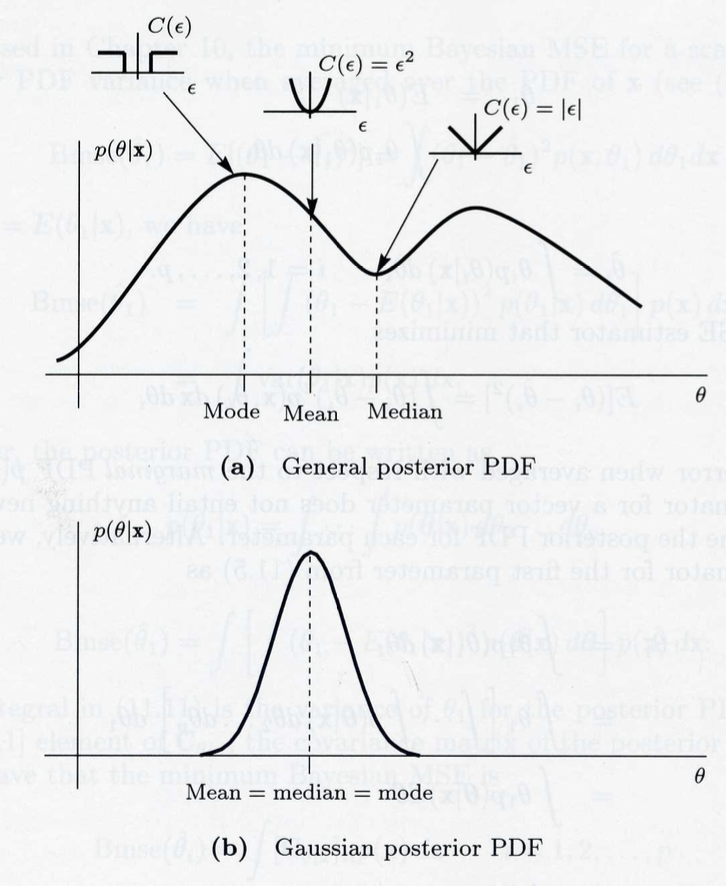
\includegraphics[width=0.3\linewidth]{Image/pdf 7/3.A-posteriori.png}
    \label{fig:placeholder}
\end{figure}
\item THe concept of Cramèr-Rao lower bound (CRB) introduced for the estimation of deterministic parameters has been also extended to the case of random parameters. It is usually called the \textbf{Bayesia CRB (BCRB)}:
\begin{align*}
\operatorname{MSE}\{\hat{Y}\}
&= E_{Y,X}\!\left\{ \bigl(Y - \hat{Y}(\mathbf{X})\bigr)^{2} \right\}
 \;\ge\; \operatorname{BCRB}(Y) = -\,\frac{1}{
   E_{Y,X}\!\left\{
      \dfrac{\partial^{2}}{\partial y^{2}}
      \ln f_{Y,X}(y,\mathbf{x})
   \right\}
 }.
\end{align*}

\item The \textbf{Bayesian CRB} is usually below the \textbf{CRB} for deterministic parameters, since the knowledge of the a-priori pdf brings additional information that allows to improve the estimation performance (if properly exploited, e.g. by deriving the MMSE estimator).
\begin{align*}
- E_{Y,X}\!\left\{
   \frac{\partial^{2}}{\partial y^{2}}
   \ln f_{Y,X}(y,\mathbf{x})
 \right\}
&= - E_{Y,X}\!\left\{
      \frac{\partial^{2}}{\partial y^{2}}
      \ln f_{X|Y}(\mathbf{x}\mid y)
      + \frac{\partial^{2}}{\partial y^{2}}
        \ln f_Y(y)
   \right\} \\[4pt]
&= - E_{Y,X}\!\left\{
      \frac{\partial^{2}}{\partial y^{2}}
      \ln f_{X|Y}(\mathbf{x}\mid y)
   \right\}
   - E_Y\!\left\{
      \frac{\partial^{2}}{\partial y^{2}}
      \ln f_Y(y)
   \right\} \\[4pt]
&= E_Y\!\left\{
      - E_{X|Y}\!\left[
        \frac{\partial^{2}}{\partial y^{2}}
        \ln f_{X|Y}(\mathbf{x}\mid y)
      \right]
   \right\}
   - E_Y\!\left\{
      \frac{\partial^{2}}{\partial y^{2}}
      \ln f_Y(y)
   \right\} \\[4pt]
&= E_Y\!\{ I(y) \}
   - E_Y\!\left\{
      \frac{\partial^{2}}{\partial y^{2}}
      \ln f_Y(y)
   \right\}
 \;\ge\; E_Y\!\{ I(y) \},
\end{align*}
\[\hspace{-2em}
\text{since}\quad
- E_Y\!\left\{
  \frac{\partial^{2}}{\partial y^{2}}
  \ln f_Y(y)
\right\} \ge 0,
\quad\text{where}\quad
I(y) \triangleq
- E_{X|Y}\!\left\{
  \frac{\partial^{2}}{\partial y^{2}}
  \ln f_{X|Y}(\mathbf{x}\mid y)
\right\}\text{ is the Fisher information.}
\]
\item Which is the MMSE estimate of a random parameter \(\theta\) if \underline{only} the \textit{a-priori} pdf of \(\theta\) is available?
\item If no data are available, we have to estimate \(\theta\) with a constant \(c\rightarrow\) Which is the value of \(c\) which minimizes the MSE?
\begin{align*}
&\hat{\theta}_{\text{ap}} = c
 \;\Rightarrow\;
\varepsilon = \theta - \hat{\theta}_{\text{ap}} = \theta - c
 \;\Rightarrow\;
\hat{\theta}_{\text{ap}} = \arg\min_{c} E\!\left\{(\theta - c)^{2}\right\}. \\[6pt]
&E\!\left\{(\theta - c)^{2}\right\}
= E\!\left\{\bigl(\theta - \eta_{\theta} + \eta_{\theta} - c\bigr)^{2}\right\}
 = E\!\left\{\bigl((\theta - \eta_{\theta}) - (c - \eta_{\theta})\bigr)^{2}\right\} \\[2pt]
&= E\!\left\{(\theta - \eta_{\theta})^{2}
          - 2(\theta - \eta_{\theta})(c - \eta_{\theta})
          + (c - \eta_{\theta})^{2}\right\} \\[2pt]
&= \sigma_{\theta}^{2} + (c - \eta_{\theta})^{2}
 \;\ge\; \sigma_{\theta}^{2}.
\end{align*}

\[
\hat{\theta}_{\text{ap}}
 = \arg\min_{c} E\!\left\{(\theta - c)^{2}\right\}
 = \eta_{\theta}
 \;\Rightarrow\;
\begin{cases}
E\{\varepsilon_{\text{ap}}\}
 = E\{\theta - \hat{\theta}_{\text{ap}}\}
 = E\{\theta - \eta_{\theta}\}
 = 0, \\[4pt]
\operatorname{MSE}\{\hat{\theta}_{\text{ap}}\}
 = E\{\varepsilon_{\text{ap}}^{2}\}
 = E\!\left\{(\theta - \eta_{\theta})^{2}\right\}
 = \sigma_{\theta}^{2}.
\end{cases}
\]
\item The Bayes estimate of a random parameter \(\theta\), when both the \textit{a-priori} pdf of \(\theta\) and the data vector \textbf{X} are available, exploits both these two "sources" of information through the \textit{a-posteriori} pdf:
\begin{align*}
\hat{\theta}_{\text{MMSE}}
&= E\{\theta \mid \mathbf{x}\}
 = \int_{-\infty}^{+\infty}
   \theta \, f_{\theta|\mathbf{X}}(\theta \mid \mathbf{x}) \, d\theta
 = \int_{-\infty}^{+\infty}
   \theta \, \frac{f_{\mathbf{X}|\theta}(\mathbf{x}\mid \theta)
                 f_{\theta}(\theta)}
                {f_{\mathbf{X}}(\mathbf{x})} \, d\theta = \frac{\displaystyle
        \int_{-\infty}^{+\infty}
        \theta \, f_{\mathbf{X}|\theta}(\mathbf{x}\mid \theta)
               f_{\theta}(\theta) \, d\theta}
        {\displaystyle
        \int_{-\infty}^{+\infty}
        f_{\mathbf{X}|\theta}(\mathbf{x}\mid \theta)
        f_{\theta}(\theta) \, d\theta}.
\end{align*}

\begin{align*}
\hat{\theta}_{\text{MAP}}
&= \arg\max_{\theta} f_{\theta|\mathbf{X}}(\theta \mid \mathbf{x})
 = \arg\max_{\theta}
   \frac{f_{\mathbf{X}|\theta}(\mathbf{x}\mid \theta)
         f_{\theta}(\theta)}
        {f_{\mathbf{X}}(\mathbf{x})} = \arg\max_{\theta}
   f_{\mathbf{X}|\theta}(\mathbf{x}\mid \theta)
   f_{\theta}(\theta)
 = \arg\max_{\theta} LF(\theta)\, f_{\theta}(\theta).
\end{align*}

\item The ML estimator of \(\theta\), modelled as a deterministic unknown paramter, relies only on the data vector \textbf{X} (but not on the \textit{a-priori} pdf of \(\theta\)):
\[
\hat{\theta}_{ML}=\underset{\theta}{\arg\max}f_{\mathbf{X}|\theta}(\mathbf{x}|\theta)=\underset{\theta}{\arg\max}LF(\theta)
\]
\end{itemize}
\subsection{Gaussian case}
\subsubsection{Single observation}
\begin{itemize}
\item Let us consider a system of 2 r.v.'s , \(X\) and \(Y\), jointly Gaussian:
\begin{align*}
f_{X,Y}(x,y)
&= \frac{1}{2\pi \sqrt{(1-\rho_{XY}^{2})\,\sigma_{X}^{2}\sigma_{Y}^{2}}}
   \exp\!\left[
      -\frac{1}{2(1-\rho_{XY}^{2})}\,Q(x,y)
   \right], \\[6pt]
Q(x,y)
&= \left(\frac{x-\eta_{X}}{\sigma_{X}}\right)^{2}
   - 2\rho_{XY}
     \left(\frac{x-\eta_{X}}{\sigma_{X}}\right)
     \left(\frac{y-\eta_{Y}}{\sigma_{Y}}\right)
   + \left(\frac{y-\eta_{Y}}{\sigma_{Y}}\right)^{2},
\end{align*}
\[
\text{where} \quad
\eta_{X} = E\{X\}, \;\;
\eta_{Y} = E\{Y\}, \;\;
\sigma_{X}^{2} = E\{(X-\eta_{X})^{2}\}, \;\;
\sigma_{Y}^{2} = E\{(Y-\eta_{Y})^{2}\},
\]
\vspace{1em}\[
\rho_{XY} = \frac{c_{XY}}{\sigma_{X}\sigma_{Y}}
 = \frac{E\{(X-\eta_{X})(Y-\eta_{Y})\}}{\sigma_{X}\sigma_{Y}}\quad\text{is the correlation coefficient between \(X\) and \(Y\)}.
\]
\begin{figure}[H]
    \centering
    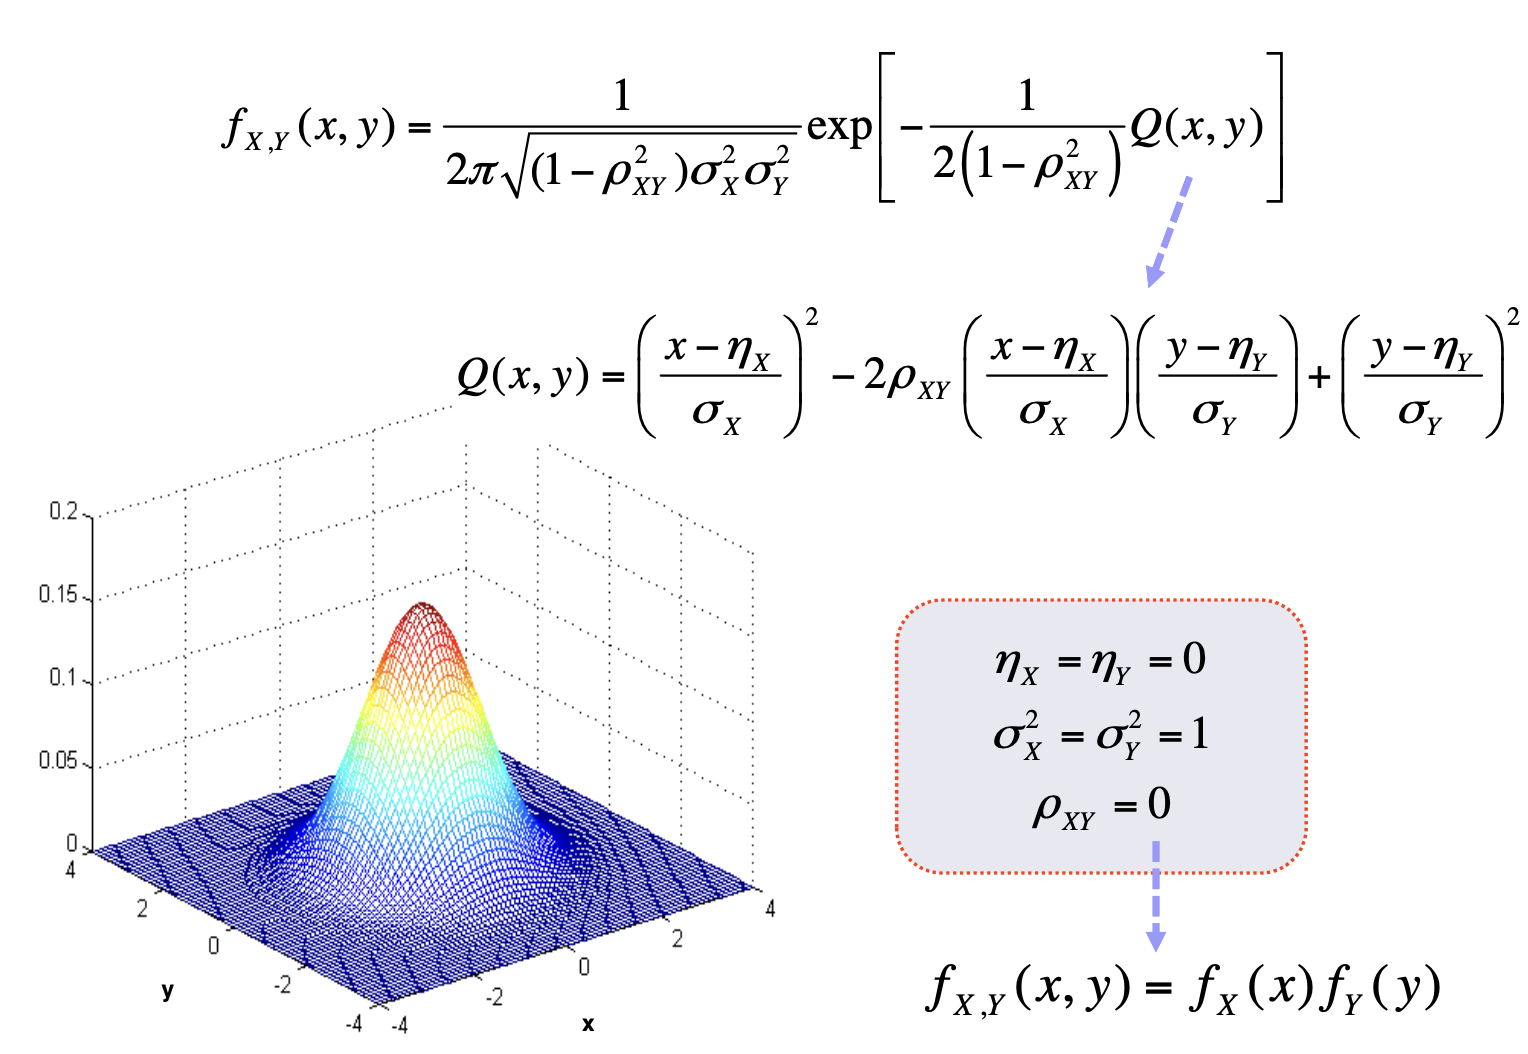
\includegraphics[width=0.65\linewidth]{Image/pdf 7/4.Gaussian_case.png}
    \label{fig:placeholder}
\end{figure}
\item \textbf{Problem}: estimate \(X\) (which is not directly observable), given the observation of \(Y\), which is correlated with \(X\) (tey are jointly Gaussian).
\item The \textbf{MMSE} estimator of \(X\) given the observed data \(Y\), in the case where \(X\) and \(Y\) are jointly Gaussian is given by the conditional mean, i.e. the mean of the a-posteriori distribution.

\begin{align*}
&\hat{X}_{\text{MMSE}}
= E\{X \mid Y\}
 = \int_{-\infty}^{+\infty} x \, f_{X|Y}(x \mid y) \, dx, \\[6pt]
&f_{X|Y}(x \mid y)
= \frac{f_{X,Y}(x,y)}{f_Y(y)}
 = \frac{\displaystyle
        \dfrac{1}{2\pi \sqrt{(1-\rho_{XY}^{2})\sigma_{X}^{2}\sigma_{Y}^{2}}}
        e^{\!
          -\frac{1}{2(1-\rho_{XY}^{2})}
          \left[
             \left(\frac{x-\eta_X}{\sigma_X}\right)^{2}
             -2\rho_{XY}\frac{x-\eta_X}{\sigma_X}\frac{y-\eta_Y}{\sigma_Y}
             +\left(\frac{y-\eta_Y}{\sigma_Y}\right)^{2}
          \right]
        }}
        {\displaystyle
        \dfrac{1}{\sqrt{2\pi\sigma_{Y}^{2}}}
        e^{\!
          -\frac{1}{2}
          \left(\frac{y-\eta_Y}{\sigma_Y}\right)^{2}
      }}
\end{align*}

\begin{align*}
f_{X|Y}(x \mid y)
&= \frac{f_{X,Y}(x,y)}{f_Y(y)} = \frac{\displaystyle
        \frac{1}{2\pi\sqrt{(1-\rho_{XY}^{2})\,\sigma_X^{2}\sigma_Y^{2}}}
        e^{\!
          -\frac{1}{2(1-\rho_{XY}^{2})}
          \left[
             \left(\frac{x-\eta_X}{\sigma_X}\right)^{2}
             -2\rho_{XY}\frac{x-\eta_X}{\sigma_X}\frac{y-\eta_Y}{\sigma_Y}
             +\left(\frac{y-\eta_Y}{\sigma_Y}\right)^{2}
          \right]
        }}
        {\displaystyle
        \frac{1}{\sqrt{2\pi\sigma_Y^{2}}}
        e^{\!
          -\frac{1}{2}
          \left(\frac{y-\eta_Y}{\sigma_Y}\right)^{2}
        }} \\[6pt]
&= \frac{1}{\sqrt{2\pi(1-\rho_{XY}^{2})\,\sigma_X^{2}}}
   e^{\!
     -\frac{1}{2(1-\rho_{XY}^{2})}
     \left[
        \left(\frac{x-\eta_X}{\sigma_X}\right)^{2}
        -2\rho_{XY}\frac{x-\eta_X}{\sigma_X}\frac{y-\eta_Y}{\sigma_Y}
        +\rho_{XY}^{2}\left(\frac{y-\eta_Y}{\sigma_Y}\right)^{2}
     \right]
  }.
\end{align*}

\begin{align*}
f_{X|Y}(x \mid y)
&= \frac{1}{\sqrt{2\pi(1-\rho_{XY}^{2})\,\sigma_X^{2}}}
   e^{\!
     -\frac{1}{2(1-\rho_{XY}^{2})}
     \left[
        \left(\frac{x-\eta_X}{\sigma_X}\right)^{2}
        -2\rho_{XY}\frac{x-\eta_X}{\sigma_X}\frac{y-\eta_Y}{\sigma_Y}
        +\rho_{XY}^{2}\left(\frac{y-\eta_Y}{\sigma_Y}\right)^{2}
     \right]
   } \\[6pt]
&= \frac{1}{\sqrt{2\pi(1-\rho_{XY}^{2})\,\sigma_X^{2}}}
   e^{\!
     -\frac{1}{2(1-\rho_{XY}^{2})\,\sigma_X^{2}}
     \left[x-\eta_X-\rho_{XY}\frac{\sigma_X}{\sigma_Y}(y-\eta_Y)\right]^{2}
   } \\[6pt]
&= \frac{1}{\sqrt{2\pi\sigma_{X|Y}^{2}}}
   e^{\!
     -\frac{(x-\eta_{X|Y})^{2}}{2\sigma_{X|Y}^{2}}
   },
\end{align*}
\begin{align*}
&\eta_{X|Y} = E\{X \mid Y\}
          = \eta_X + \rho_{XY}\frac{\sigma_X}{\sigma_Y}(Y-\eta_Y)\quad\longrightarrow\quad\text{Regression Line}\\[4pt]
&\sigma_{X|Y}^{2}
= \operatorname{var}\{X \mid Y\}=E\{(X-\eta_{X\mid Y})^2\mid Y\}=E\{X^2\mid Y\}-(E\{X^2\mid Y\})^2
= \sigma_X^{2}(1-\rho_{XY}^{2})
\end{align*}

\item The \textbf{MMSE} estimator of \(X\) given the observed data \(Y\), in the case where \(X\) and \(Y\) are jointly Gaussian r.v.'s is given by:

\begin{align*}
\hat{X}_{\text{MMSE}}
&= E\{X \mid Y\}
 = \eta_{X|Y}
 = \eta_X + \rho_{XY}\frac{\sigma_X}{\sigma_Y}(Y-\eta_Y). \\[8pt]
\operatorname{MSE}\{\hat{X}_{\text{MMSE}}\}
&= E_{Y,X}\!\left\{ (X-\hat{X}_{\text{MMSE}})^{2} \right\}
 = E_Y\!\left\{ E_{X|Y}\!\left[ (X-\hat{X}_{\text{MMSE}})^{2} \mid Y \right] \right\} \\[4pt]
&= E_Y\!\left\{ E_{X|Y}\!\left[ (X-\eta_{X|Y})^{2} \mid Y \right] \right\}
 = E_Y\!\left\{ \operatorname{var}\{X \mid Y\} \right\} \\[4pt]
&= E_Y\!\left\{ \sigma_{X|Y}^{2} \right\}
 = E_Y\!\left\{ \sigma_X^{2}(1-\rho_{XY}^{2}) \right\}
 = \sigma_X^{2}(1-\rho_{XY}^{2}).
\end{align*}

\item The conditional mean and conditional variance can also be expressed in terms of the \underline{covariance} between \(X\) and \(Y\):

\begin{align*}
\eta_{X|Y}
&= \eta_X + \rho_{XY}\frac{\sigma_X}{\sigma_Y}(Y-\eta_Y)
 = \eta_X + \rho_{XY}\frac{\sigma_X\sigma_Y}{\sigma_Y^{2}}(Y-\eta_Y)  = \eta_X + c_{XY}\,(\sigma_Y^{2})^{-1}(Y-\eta_Y), \\[8pt]
\sigma_{X|Y}^{2}
&= \sigma_X^{2}(1-\rho_{XY}^{2})
 = \sigma_X^{2}\!\left(1-\frac{c_{XY}^{2}}{\sigma_X^{2}\sigma_Y^{2}}\right)
 = \sigma_X^{2} - \frac{c_{XY}^{2}}{\sigma_Y^{2}} = \sigma_X^{2} - c_{XY}\,(\sigma_Y^{2})^{-1}c_{XY}.
\end{align*}

\item \textbf{Example}: Observed data = Signal+Noise \(\rightarrow\)\quad Y+W
\begin{align*}
S &\in \mathcal{N}(\eta_S,\sigma_S^{2}), \qquad
W \in \mathcal{N}(0,\sigma_W^{2}), \qquad
S \text{ and } W \text{ independent}, \\[6pt]
\operatorname{SNR}
&= \frac{E\{S^{2}\}}{E\{W^{2}\}}
 = \frac{\eta_S^{2}+\sigma_S^{2}}{\sigma_W^{2}}
 = \frac{\sigma_S^{2}}{\sigma_W^{2}}
   \left(1+\frac{\eta_S^{2}}{\sigma_S^{2}}\right)
 = \gamma (1+\kappa),
\end{align*}

\item Find the \textbf{MMSE estimator} of the random signal \(S\) given the observed data \(Y\): we should derive the pdf of \(S\) given \(Y\) (the so-called \textit{a-posteriori} pdf).
\item Since \(S\) and \(Y\) are jointly Gaussian, we already know that the pdf of \(S\) given \(Y\) is a Gaussian pdf, so we can derive directly the conditional mean and variance by using the previous results.

\begin{align*}
\hat{S}_{\text{MMSE}}
&= E\{S \mid Y\}
 = \eta_S + \rho_{YS}\frac{\sigma_S}{\sigma_Y}(Y-\eta_Y), \\[6pt]
\eta_Y &= E\{Y\} = E\{S+W\} = \eta_S, \\[4pt]
\sigma_Y^{2}
&= \operatorname{var}\{Y\}
 = \operatorname{var}\{S+W\}
 = \sigma_S^{2} + \sigma_W^{2}
 = \sigma_W^{2}(1+\gamma), \\[6pt]
\rho_{YS}
&= \frac{\operatorname{cov}\{Y,S\}}
        {\sqrt{\sigma_Y^{2}\sigma_S^{2}}}
 = \frac{E\{(Y-\eta_Y)(S-\eta_S)\}}
        {\sqrt{\sigma_S^{2}(\sigma_S^{2}+\sigma_W^{2})}} \\[4pt]
&= \frac{E\{(S+W-\eta_S)(S-\eta_S)\}}
        {\sqrt{\sigma_S^{2}(\sigma_S^{2}+\sigma_W^{2})}}
 = \frac{\sigma_S^{2}}
        {\sqrt{\sigma_S^{2}(\sigma_S^{2}+\sigma_W^{2})}}
 = \sqrt{\frac{\sigma_S^{2}}{\sigma_S^{2}+\sigma_W^{2}}}
 = \sqrt{\frac{\gamma}{\gamma+1}}\\
\end{align*}
\vspace{-1em}
\[\hat{S}_{MMSE}=\alpha Y+ (1-\alpha)\eta_S\]\vspace{-0.5em}
\[\text{with } \gamma \triangleq \dfrac{\sigma_S^{2}}{\sigma_W^{2}}\qquad \alpha\triangleq\frac{\gamma}{\gamma+1}\]

\item Hence:
\begin{align*}
\hat{S}_{\text{MMSE}}
&= \alpha Y + (1-\alpha)\eta_S,
\qquad
\text{where } \alpha \triangleq \frac{\gamma}{\gamma+1},
\;\; \gamma \triangleq \frac{\sigma_S^{2}}{\sigma_W^{2}}. \\[8pt]
\operatorname{MSE}\{\hat{S}_{\text{MMSE}}\}
&= \sigma_S^{2}(1-\rho_{YS}^{2})
 = \sigma_S^{2}\!\left(1-\frac{\gamma}{\gamma+1}\right)
 = (1-\alpha)\sigma_S^{2}. \\[8pt]
\operatorname{MSE}\{\hat{S}_{\text{MMSE}}\}
&= (1-\alpha)\,\operatorname{MSE}\{\hat{S}_{\text{ap}}\}
 \le \operatorname{MSE}\{\hat{S}_{\text{ap}}\}, \\[4pt]
\operatorname{MSE}\{\hat{S}_{\text{MMSE}}\}
&= \operatorname{MSE}\{\hat{S}_{\text{ap}}\}
 \;\Longleftrightarrow\;
\gamma \to 0
\;(\sigma_S^{2}\to 0 \text{ or } \sigma_W^{2}\to +\infty).
\end{align*}
\item Let us compare the \textbf{MMSE} estimator with the \textbf{ML} estimator:
\begin{align*}
\hat{S}_{\text{ML}}
&= \arg\max_{s} \ln f_{Y|S}(y \mid s)
 = Y,
\qquad \text{since } Y \mid S \in \mathcal{N}(S,\sigma_W^{2}). \\[8pt]
\operatorname{MSE}\{\hat{S}_{\text{ML}}\}
&= E\!\left\{(S-\hat{S}_{\text{ML}})^{2}\right\}
 = E\!\left\{(S-Y)^{2}\right\}
 = E\{W^{2}\}
 = \sigma_W^{2}. \\[8pt]
\operatorname{MSE}\{\hat{S}_{\text{MMSE}}\}
&= \sigma_S^{2}\!\left(1-\frac{\gamma}{\gamma+1}\right)
 = \sigma_S^{2}\!\left(1-\frac{\sigma_S^{2}}{\sigma_S^{2}+\sigma_W^{2}}\right)= \frac{\sigma_W^{2}\sigma_S^{2}}{\sigma_W^{2}+\sigma_S^{2}}
 = \frac{\gamma}{\gamma+1}\,\sigma_W^{2}
 = \alpha \sigma_W^{2}\\[4pt]
\operatorname{MSE}\{\hat{S}_{\text{MMSE}}\}&= \alpha\operatorname{MSE}\{\hat{S}_{\text{ML}}\}
 \le \operatorname{MSE}\{\hat{S}_{\text{ML}}\}\\[8pt]
\operatorname{MSE}\{\hat{S}_{\text{MMSE}}\}
 &= \operatorname{MSE}\{\hat{S}_{\text{ML}}\}
 \;\Longleftrightarrow\;
\gamma \to +\infty
\;(\sigma_S^{2}\to +\infty \text{ or } \sigma_W^{2}\to 0).
\end{align*}

\item In summary:
\begin{align*}
&\hat{S}_{\text{MMSE}}
= \alpha Y + (1-\alpha)\eta_S
 = \alpha \hat{S}_{\text{ML}} + (1-\alpha)\hat{S}_{\text{ap}},
\qquad
\alpha \triangleq \frac{\gamma}{\gamma+1},
\;\; \gamma \triangleq \frac{\sigma_S^{2}}{\sigma_W^{2}}, \\[8pt]
&\operatorname{MSE}\{\hat{S}_{\text{MMSE}}\}
= (1-\alpha)\sigma_S^{2}
 = (1-\alpha)\operatorname{MSE}\{\hat{S}_{\text{ap}}\}
 = \alpha\sigma_W^{2}
 = \alpha\,\operatorname{MSE}\{\hat{S}_{\text{ML}}\}. \\[10pt]
&\sigma_S^{2} = \text{const.}\quad
\begin{cases}
\sigma_W^{2} \to +\infty
 &\Rightarrow \gamma = \dfrac{\sigma_S^{2}}{\sigma_W^{2}} \to 0
  \Rightarrow \alpha \to 0
  \Rightarrow
  \begin{cases}
  \hat{S}_{\text{MMSE}} \to \eta_S, \\[8pt]
  \operatorname{MSE}\{\hat{S}_{\text{MMSE}}\} \to \sigma_S^{2};
  \end{cases} \\[20pt]
\sigma_W^{2} \to 0
 &\Rightarrow \gamma = \dfrac{\sigma_S^{2}}{\sigma_W^{2}} \to +\infty
  \Rightarrow \alpha \to 1
  \Rightarrow
  \begin{cases}
  \hat{S}_{\text{MMSE}} \to Y = S, \\[8pt]
  \operatorname{MSE}\{\hat{S}_{\text{MMSE}}\} \to 0.
  \end{cases}
\end{cases}
\end{align*}
\end{itemize}
\subsubsection{Multiple observations}

\begin{itemize}
    \item Let us now consider the system formed by 2 vectors \textbf{X} and \textbf{Y}, jointly Gaussian and mutually correlated. The joint pdf of \textbf{X} and \textbf{Y} is derived as follows:

\begin{align*}
&{X}_{k\times 1} \in \mathcal{N}(\eta_X, C_X), \qquad
Y_{l\times 1} \in \mathcal{N}(\eta_Y, C_Y),\qquad
C_{XY} = E\!\left\{(X-\eta_X)(Y-\eta_Y)^{T}\right\}. \\[8pt]
&Z_{(k+l)\times 1}
= \begin{bmatrix} X \\ Y \end{bmatrix}
 \;\Rightarrow\;
Z \in \mathcal{N}(\eta_Z, C_Z), \\[6pt]
&\underset{(k+l)\times 1}{\eta_Z}
= E\{Z\}
 = E\!\left\{\begin{bmatrix} X \\ Y \end{bmatrix}\right\}
 = \begin{bmatrix} \eta_X \\ \eta_Y \end{bmatrix}, \\[8pt]
&\underset{(k+l)\times(k+l)}{C_Z}
= E\!\left\{(Z-\eta_Z)(Z-\eta_Z)^{T}\right\}= E\!\left\{
   \left(
     \begin{bmatrix} X \\ Y \end{bmatrix}
     - \begin{bmatrix} \eta_X \\ \eta_Y \end{bmatrix}
   \right)
   \left(
     \begin{bmatrix} X \\ Y \end{bmatrix}
     - \begin{bmatrix} \eta_X \\ \eta_Y \end{bmatrix}
   \right)^{T}
  \right\}.
\end{align*}
\begin{align*}
C_Z
&= E\!\left\{
   \begin{bmatrix} X-\eta_X \\[2pt] Y-\eta_Y \end{bmatrix}
   \begin{bmatrix} X-\eta_X \\[2pt] Y-\eta_Y \end{bmatrix}^{T}
 \right\} = E\!\left\{
   \begin{bmatrix} X-\eta_X \\[2pt] Y-\eta_Y \end{bmatrix}
   \bigl[(X-\eta_X)^{T}\ (Y-\eta_Y)^{T}\bigr]
 \right\} \\[6pt]
&= E\!\left\{
   \begin{bmatrix}
     (X-\eta_X)(X-\eta_X)^{T} & (X-\eta_X)(Y-\eta_Y)^{T} \\
     (Y-\eta_Y)(X-\eta_X)^{T} & (Y-\eta_Y)(Y-\eta_Y)^{T}
   \end{bmatrix}
 \right\} =
\begin{bmatrix}
  C_X  & C_{XY} \\
  C_{YX} & C_Y
\end{bmatrix},
\end{align*}
where
\[
C_{XY} \triangleq E\!\left\{(X-\eta_X)(Y-\eta_Y)^{T}\right\},
\qquad
C_{YX} = C_{XY}^{T}.
\]

\[
f_Z(z) \equiv f_{X,Y}(x,y)
 = \frac{1}{(2\pi)^{\frac{k+l}{2}}\sqrt{|C_Z|}}
   \exp\!\left[
     -\frac{1}{2}
     \begin{bmatrix} x-\eta_X \\ y-\eta_Y \end{bmatrix}^{T}
     C_Z^{-1}
     \begin{bmatrix} x-\eta_X \\ y-\eta_Y \end{bmatrix}
   \right].
\]

    \item It can be proved that the pdf of \textbf{X} given \textbf{Y} is a multidimentsional \textbf{Gaussian pdf}:
    \begin{align*}
\mathbf{f}_{X|Y}(\mathbf{x}\mid\mathbf{y})
&= \frac{\mathbf{f}_{X,Y}(\mathbf{x},\mathbf{y})}{\mathbf{f}_Y(\mathbf{y})} \\[4pt]
&= \frac{1}{(2\pi)^{k/2}\sqrt{\lvert \mathbf{C}_{X|Y}\rvert}}
   \exp\!\left[
     -\frac{1}{2}
     (\mathbf{x}-\boldsymbol{\eta}_{X|Y})^{T}
     \mathbf{C}_{X|Y}^{-1}
     (\mathbf{x}-\boldsymbol{\eta}_{X|Y})
   \right].
\end{align*}
\item With \textbf{mean vector} and \textbf{covariance matrix} is given by:

\item That are very similar to those derived in the scalar case.
\begin{align*}
\boldsymbol{\eta}_{X|Y}
&= E\{\mathbf{X}\mid\mathbf{Y}\}
 = \boldsymbol{\eta}_X
   + \mathbf{C}_{XY}\,\mathbf{C}_Y^{-1}\,(\mathbf{Y}-\boldsymbol{\eta}_Y)
 \qquad\text{[It is a \textbf{linear} function of }\mathbf{Y}\text{]}, \\[10pt]
\mathbf{C}_{X|Y}
&= E\!\left\{(\mathbf{X}-\boldsymbol{\eta}_{X|Y})
            (\mathbf{X}-\boldsymbol{\eta}_{X|Y})^{T}\mid\mathbf{Y}\right\} \\
&= \mathbf{C}_X - \mathbf{C}_{XY}\,\mathbf{C}_Y^{-1}\,\mathbf{C}_{YX}
 = \mathbf{C}_X - \mathbf{C}_{YX}^{T}\,\mathbf{C}_Y^{-1}\,\mathbf{C}_{YX}.
\end{align*}

\item The gaussian vector case is a straightforward generalization of the Gaussian scalar case:
\[
\begin{cases}
    \eta_{X\mid Y}=\eta_X+c_{XY}(\sigma_Y^2)^{-1}(Y-\eta_Y)\\[6pt]
    \sigma_{X\mid Y}^2=\sigma_X^2-c_{XY}(\sigma^2_Y)^{-1}c_{YX}
\end{cases}\quad\Longrightarrow\quad
\begin{cases}
\boldsymbol{\eta}_{X|Y}
= \boldsymbol{\eta}_X
   + \mathbf{C}_{XY}\,\mathbf{C}_Y^{-1}\,(\mathbf{Y}-\boldsymbol{\eta}_Y), \\[6pt]
\mathbf{C}_{X|Y}
= \mathbf{C}_X - \mathbf{C}_{XY}\,\mathbf{C}_Y^{-1}\,\mathbf{C}_{YX}
 = \mathbf{C}_X - \mathbf{C}_{YX}^{T}\,\mathbf{C}_Y^{-1}\,\mathbf{C}_{YX}.
\end{cases}
\]

\item This means that the \textbf{MMSE estimate} of vector \textbf{X} given the observed data vector \textbf{Y}, when then vectors \textbf{X} and \textbf{Y} are \textbf{jointly gaussian} distributed, is given by:
\begin{align*}
\hat{\mathbf{X}}_{\text{MMSE}}
&= \boldsymbol{\eta}_{X|Y}
 = E\{\mathbf{X}\mid\mathbf{Y}\}
 = \boldsymbol{\eta}_X
   + \mathbf{C}_{XY}\,\mathbf{C}_Y^{-1}\,(\mathbf{Y}-\boldsymbol{\eta}_Y)
\end{align*}
\item The MMSE estimator is \textbf{linear}, hence it is \textbf{Gaussian} distributed.
\item The \textbf{MSE matrix} is obtained by averaging with respect to the observed data vector the conditional covariance matrix:
\begin{align*}
\operatorname{\mathbf{MSE}}\!\left\{\hat{\mathbf{X}}_{\text{MMSE}}\right\}= E_{\mathbf{Y}}\!\left\{\mathbf{C}_{X|Y}\right\}= E_{\mathbf{Y}}\!\left\{\mathbf{C}_X
      - \mathbf{C}_{YX}^{T}\mathbf{C}_Y^{-1}\mathbf{C}_{YX}\right\}= \mathbf{C}_X - \mathbf{C}_{YX}^{T}\mathbf{C}_Y^{-1}\mathbf{C}_{YX}.
\end{align*}
\item It can be proved that in the Gaussian case, it coincides with the \textbf{Bayes CRB}.
\end{itemize}
\subsection{The Bayesian Linear Model}
\begin{itemize}
\item We have introduced the \textbf{Deterministic Linear Model}, which applies when the useful signal \textbf{S} can be expressed as the linear combination of \(p\) vectors \(\{\textbf{h}_i\}\), i.e. \textbf{S} belongs to the subspace generated by the \(p\) vectors \(\{\mathbf{h}_i\}\), with \(p<N\):
\begin{align*}
\underset{N\times 1}{\mathbf{Y}}
&= \mathbf{S} + \mathbf{W}
 = \mathbf{H}\boldsymbol{\theta} + \mathbf{W}
 = \sum_{i=1}^{p}\theta_i\,\mathbf{h}_i + \mathbf{W}, \\[6pt]
\underset{N\times p}{\mathbf{H}}
&= [\,\mathbf{h}_1\ \mathbf{h}_2\ \dots\ \mathbf{h}_p\,], \quad
\underset{p\times 1}{\boldsymbol{\theta}}
 = \begin{bmatrix}\theta_1 \\ \theta_2 \\ \vdots \\ \theta_p\end{bmatrix},\quad \mathbf{W} \in \mathcal{N}(\mathbf{0},\mathbf{C}_W), \quad
\mathbf{C}_W = E\{\mathbf{W}\mathbf{W}^{T}\}.
\end{align*}

\item \textbf{Problem}: estimate \(\theta\) given the observed data vector \textbf{Y}, assuming that \textbf{H} is perfectly known.
\[
\underset{N\times 1}{\mathbf{Y}}
= \mathbf{H}\boldsymbol{\theta} + \mathbf{W}
= \sum_{i=1}^{p}\theta_i\,\mathbf{h}_i + \mathbf{W}.
\]

\item We have seen that when \(\theta\) is modelled as a vector of \textbf{deterministic unknown parameters} and the additive noise is Gaussian, we can resort to the \textbf{ML method} to estimate \(\theta\):
\begin{align*}
\hat{\boldsymbol{\theta}}_{\text{ML}}
&= \arg\max_{\boldsymbol{\theta}} \ln f_{\mathbf{Y}}(\mathbf{y};\boldsymbol{\theta})= \left(\mathbf{H}^{T}\mathbf{C}_W^{-1}\mathbf{H}\right)^{-1}
    \mathbf{H}^{T}\mathbf{C}_W^{-1}\mathbf{Y}.
\end{align*}

\item Note that the estimator is \textbf{linear}, it is also called \textbf{Blue}.

\item The \textbf{ML estimator} of \(\theta\) is \textbf{linear}, \textbf{unbiased},\textbf{Gaussian}, \textbf{efficient}, and \textbf{consistent}:
\[
\begin{cases}
\hat{\boldsymbol{\theta}}_{\text{ML}}
= \left(\mathbf{H}^{T}\mathbf{C}_W^{-1}\mathbf{H}\right)^{-1}
    \mathbf{H}^{T}\mathbf{C}_W^{-1}\mathbf{Y}, \\[6pt]
E\{\hat{\boldsymbol{\theta}}_{\text{ML}}\}
= \boldsymbol{\theta}, \\[6pt]
\operatorname{MSE}\{\hat{\boldsymbol{\theta}}_{\text{ML}}\}
= \operatorname{CRB}(\boldsymbol{\theta})
 = \left(\mathbf{H}^{T}\mathbf{C}_W^{-1}\mathbf{H}\right)^{-1}, \\[6pt]
\end{cases}\]
\vspace{-0.5em}
\[
\hat{\boldsymbol{\theta}}_{\text{ML}}
\in \mathcal{N}\!\left(\boldsymbol{\theta},\operatorname{CRB}(\boldsymbol{\theta})\right).
\]
\item \underline{\textbf{Assumption}}: vector \(\theta\) can be modelled as a random vector with known mean vector and covariance matrix \(\rightarrow\) the \underline{\textbf{Bayesian linear model}}.
\item If we assume that it is Gaussian distributed: 
\[
\boldsymbol{\theta}\in\mathcal{N}(\boldsymbol{\eta}_{\theta},\textbf{C}_{\theta})\quad\rightarrow\quad \text{the }\textbf{Gaussian linear model}
\]
\item \textbf{Problem}: find the \textbf{MMSE} estimator of \(\theta\) given the observed data vector \textbf{Y}, assuming that the matrix \textbf{H} is a-priori perfectly known and that \(\theta\) can be modelled as a \textbf{Gaussian} random vector with known pdf: \(\boldsymbol{\theta}\in\mathcal{N}(\boldsymbol{\eta}_{\theta},\mathbf{C}_{\theta})\)
\begin{align*}
&\underset{N\times 1}{\mathbf{Y}}
= \mathbf{H}\boldsymbol{\theta} + \mathbf{W}
 = \sum_{i=1}^{p}\theta_i\,\mathbf{h}_i + \mathbf{W}, \\[6pt]
&\underset{N\times p}{\mathbf{H}}
= [\,\mathbf{h}_1\ \mathbf{h}_2\ \dots\ \mathbf{h}_p\,], \qquad
\boldsymbol{\theta}_{p\times 1}
 = \begin{bmatrix}\theta_1 \\ \theta_2 \\ \vdots \\ \theta_p\end{bmatrix},\quad\mathbf{W} \in \mathcal{N}(\mathbf{0},\mathbf{C}_W),
\quad
\mathbf{C}_W = E\{\mathbf{W}\mathbf{W}^{T}\}, \\[8pt]
&\underset{N\times 1}{\mathbf{S}}
= \mathbf{H}\boldsymbol{\theta}
\quad\text{(signal of interest, Gaussian random vector)}\quad \rightarrow\quad\hat{\mathbf{S}}_{\text{MMSE}}
= \mathbf{H}\,\hat{\boldsymbol{\theta}}_{\text{MMSE}}.
\end{align*}
\item Next step:
\begin{align*}
\boldsymbol{\theta} &\in \mathcal{N}(\boldsymbol{\eta}_\theta,\mathbf{C}_\theta),
\qquad
\mathbf{Y}\mid\boldsymbol{\theta} \in \mathcal{N}(\mathbf{H}\boldsymbol{\theta},\mathbf{C}_W), \\[6pt]
f_{\mathbf{Y}\mid\boldsymbol{\theta}}(\mathbf{y}\mid\boldsymbol{\theta})
&= \frac{1}{\sqrt{(2\pi)^N\lvert\mathbf{C}_W\rvert}}
   \exp\!\left(
     -\frac{1}{2}(\mathbf{y}-\mathbf{H}\boldsymbol{\theta})^{T}
              \mathbf{C}_W^{-1}
              (\mathbf{y}-\mathbf{H}\boldsymbol{\theta})
   \right), \\[10pt]
\mathbf{Y} &\in \mathcal{N}(\boldsymbol{\eta}_Y,\mathbf{C}_Y), \\[4pt]
\boldsymbol{\eta}_Y
&= E\{\mathbf{Y}\}
 = E\{\mathbf{S}+\mathbf{W}\}
 = E\{\mathbf{H}\boldsymbol{\theta}\}
 = \mathbf{H}E\{\boldsymbol{\theta}\}
 = \mathbf{H}\boldsymbol{\eta}_\theta, \\[8pt]
\mathbf{C}_Y
&= E\!\left\{(\mathbf{Y}-\boldsymbol{\eta}_Y)
            (\mathbf{Y}-\boldsymbol{\eta}_Y)^{T}\right\} = E\!\left\{(\mathbf{H}\boldsymbol{\theta}+\mathbf{W}-\mathbf{H}\boldsymbol{\eta}_\theta)
            (\mathbf{H}\boldsymbol{\theta}+\mathbf{W}-\mathbf{H}\boldsymbol{\eta}_\theta)^{T}\right\} \\[2pt]
&= E\!\left\{(\mathbf{H}(\boldsymbol{\theta}-\boldsymbol{\eta}_\theta)+\mathbf{W})
            (\mathbf{H}(\boldsymbol{\theta}-\boldsymbol{\eta}_\theta)+\mathbf{W})^{T}\right\} = E\!\left\{\mathbf{H}(\boldsymbol{\theta}-\boldsymbol{\eta}_\theta)
              (\boldsymbol{\theta}-\boldsymbol{\eta}_\theta)^{T}\mathbf{H}^{T}\right\}
   + E\{\mathbf{W}\mathbf{W}^{T}\} \\[2pt]
&= \mathbf{H}\mathbf{C}_\theta\mathbf{H}^{T} + \mathbf{C}_W.
\end{align*}
\item After, we can obtain:
\begin{align*}
f_{\boldsymbol{\theta}\mid\mathbf{Y}}(\boldsymbol{\theta}\mid\mathbf{y})
&= \frac{f_{\mathbf{Y}\mid\boldsymbol{\theta}}(\mathbf{y}\mid\boldsymbol{\theta})
        f_{\boldsymbol{\theta}}(\boldsymbol{\theta})}
       {f_{\mathbf{Y}}(\mathbf{y})}
 = \frac{1}{\sqrt{(2\pi)^{p}\lvert\mathbf{C}_{\boldsymbol{\theta}\mid\mathbf{Y}}\rvert}}
   \exp\!\left(
     -\frac{1}{2}
     (\boldsymbol{\theta}-\boldsymbol{\eta}_{\boldsymbol{\theta}\mid\mathbf{Y}})^{T}
     \mathbf{C}_{\boldsymbol{\theta}\mid\mathbf{Y}}^{-1}
     (\boldsymbol{\theta}-\boldsymbol{\eta}_{\boldsymbol{\theta}\mid\mathbf{Y}})
   \right), \\[10pt]
\boldsymbol{\eta}_{\boldsymbol{\theta}\mid\mathbf{Y}}
&= E\{\boldsymbol{\theta}\mid\mathbf{Y}\}
 = \boldsymbol{\eta}_\theta
   + \mathbf{C}_{\boldsymbol{\theta}\mathbf{Y}}\mathbf{C}_Y^{-1}
     (\mathbf{Y}-\boldsymbol{\eta}_Y), \\[6pt]
\mathbf{C}_{\boldsymbol{\theta}\mid\mathbf{Y}}
&= E\!\left\{
   (\boldsymbol{\theta}-\boldsymbol{\eta}_{\boldsymbol{\theta}\mid\mathbf{Y}})
   (\boldsymbol{\theta}-\boldsymbol{\eta}_{\boldsymbol{\theta}\mid\mathbf{Y}})^{T}
   \mid \mathbf{Y}
  \right\} \\[2pt]
&= \mathbf{C}_\theta
   - \mathbf{C}_{\boldsymbol{\theta}\mathbf{Y}}
     \mathbf{C}_Y^{-1}
     \mathbf{C}_{\mathbf{Y}\boldsymbol{\theta}}, \\[8pt]
\text{where}\quad
\boldsymbol{\eta}_Y &= \mathbf{H}\boldsymbol{\eta}_\theta,
\qquad
\mathbf{C}_Y = \mathbf{H}\mathbf{C}_\theta\mathbf{H}^{T} + \mathbf{C}_W, \\[4pt]
\mathbf{C}_{\boldsymbol{\theta}\mathbf{Y}}
&= (\mathbf{C}_{\mathbf{Y}\boldsymbol{\theta}})^{T}
 = E\{(\boldsymbol{\theta}-\boldsymbol{\eta}_\theta)
      (\mathbf{Y}-\boldsymbol{\eta}_Y)^{T}\} \\[2pt]
&= E\{(\boldsymbol{\theta}-\boldsymbol{\eta}_\theta)
      (\mathbf{H}(\boldsymbol{\theta}-\boldsymbol{\eta}_\theta)+\mathbf{W})^{T}\} \\[2pt]
&= E\{(\boldsymbol{\theta}-\boldsymbol{\eta}_\theta)
      (\boldsymbol{\theta}-\boldsymbol{\eta}_\theta)^{T}\mathbf{H}^{T}\}
 = \mathbf{C}_\theta\mathbf{H}^{T}.
\end{align*}

\item Hence, we find:
\begin{align*}
\boldsymbol{\eta}_{\boldsymbol{\theta}\mid\mathbf{Y}}
&= \boldsymbol{\eta}_\theta
   + \mathbf{C}_\theta\mathbf{H}^{T}
     \left(\mathbf{H}\mathbf{C}_\theta\mathbf{H}^{T}
           + \mathbf{C}_W\right)^{-1}
     (\mathbf{Y}-\mathbf{H}\boldsymbol{\eta}_\theta), \\[10pt]
\mathbf{C}_{\boldsymbol{\theta}\mid\mathbf{Y}}
&= \mathbf{C}_\theta
   - \mathbf{C}_\theta\mathbf{H}^{T}
     \left(\mathbf{H}\mathbf{C}_\theta\mathbf{H}^{T}
           + \mathbf{C}_W\right)^{-1}
     \mathbf{H}\mathbf{C}_\theta.
\end{align*}
\item Using the \textbf{Matrix inversion Lemma}, they can be expressed as :

\begin{align*}
\boldsymbol{\eta}_{\boldsymbol{\theta}\mid\mathbf{Y}}
&= \boldsymbol{\eta}_\theta
   + \left(\mathbf{C}_\theta^{-1}
           + \mathbf{H}^{T}\mathbf{C}_W^{-1}\mathbf{H}\right)^{-1}
     \mathbf{H}^{T}\mathbf{C}_W^{-1}
     (\mathbf{Y}-\mathbf{H}\boldsymbol{\eta}_\theta), \\[10pt]
\mathbf{C}_{\boldsymbol{\theta}\mid\mathbf{Y}}
&= \left(\mathbf{C}_\theta^{-1}
         + \mathbf{H}^{T}\mathbf{C}_W^{-1}\mathbf{H}\right)^{-1}.
\end{align*}
\item \underline{\textbf{Matrix Inversion Lemma (a.k.a Woodbury Identity)}}
\[
\left( \mathbf{A} + \mathbf{B}\mathbf{D}^{-1}\mathbf{C} \right)^{-1}
= \mathbf{A}^{-1} - \mathbf{A}^{-1}\mathbf{B}
\left( \mathbf{D} + \mathbf{C}\mathbf{A}^{-1}\mathbf{B} \right)^{-1}
\mathbf{C}\mathbf{A}^{-1}
\]
\noindent Where \textbf{A} and \textbf{D} are square matrices of full rank and \textbf{B} and \textbf{C} are rectangular matrices of proper dimensions.
$$\mathbf{A} = \mathbf{C}_\theta^{-1},\ \mathbf{B} = \mathbf{H}^T,\ \mathbf{C} = \mathbf{H},\ \mathbf{D} = \mathbf{C}_w$$

$$\left( \mathbf{C}_\theta^{-1} + \mathbf{H}^T \mathbf{C}_w^{-1} \mathbf{H} \right)^{-1}
= \mathbf{C}_\theta - \mathbf{C}_\theta \mathbf{H}^T \left( \mathbf{C}_w + \mathbf{H} \mathbf{C}_\theta \mathbf{H}^T \right)^{-1} \mathbf{H} \mathbf{C}_\theta$$

\item \underline{\textbf{Woodbury identity}}(it comes in may variants):

$$\left( \mathbf{P}^{-1} + \mathbf{B}^T \mathbf{R}^{-1} \mathbf{B} \right)^{-1} \mathbf{B}^T \mathbf{R}^{-1}
= \mathbf{P} \mathbf{B}^T \left( \mathbf{B} \mathbf{P} \mathbf{B}^T + \mathbf{R} \right)^{-1}$$


\noindent Where \textbf{P} and \textbf{R} are square matrices of full rank and \textbf{B} a rectangular matrix of proper dimensions.
$$\mathbf{P} = \mathbf{C}_\theta,\ \mathbf{B} = \mathbf{H},\ \mathbf{R} = \mathbf{C}_w$$

$$\mathbf{C}_\theta \mathbf{H}^T \left( \mathbf{H} \mathbf{C}_\theta \mathbf{H}^T + \mathbf{C}_w \right)^{-1}
= \left( \mathbf{C}_\theta^{-1} + \mathbf{H}^T \mathbf{C}_w^{-1} \mathbf{H} \right)^{-1} \mathbf{H}^T \mathbf{C}_w^{-1}$$

\item In summary, the \textbf{MMSE} estimator of the Gaussian random vector \(\theta\) and the covariance matrix of the estimation error (which coincides with the BCRB) are:
\begin{align*}
&\hat{\boldsymbol{\theta}}_{MMSE} = \boldsymbol{\eta}_{\boldsymbol{\theta}|\mathbf{Y}} = \boldsymbol{\eta}_{\boldsymbol{\theta}} + \left(\mathbf{C}_{\boldsymbol{\theta}}^{-1} + \mathbf{H}^{T} \mathbf{C}_{\mathbf{W}}^{-1} \mathbf{H}\right)^{-1} \mathbf{H}^{T} \mathbf{C}_{\mathbf{W}}^{-1} \left(\mathbf{Y} - \mathbf{H} \boldsymbol{\eta}_{\boldsymbol{\theta}}\right) \\[1em]
&MSE\left\{\hat{\boldsymbol{\theta}}_{MMSE}\right\} = \mathbf{C}_{\boldsymbol{\theta}|\mathbf{Y}} = \left(\mathbf{C}_{\boldsymbol{\theta}}^{-1} + \mathbf{H}^{T} \mathbf{C}_{\mathbf{W}}^{-1} \mathbf{H}\right)^{-1} = \mathbf{BCRB}(\boldsymbol{\theta})
\end{align*}
\item The \textbf{MMSE estimator} of the parameters of the \textbf{Gaussian linear model} is a \textbf{linear} function of the data vector \textbf{Y}, it is \textbf{efficient} and \textbf{unbiased}: 
\begin{align*}
E\left\{\boldsymbol{\theta} - \hat{\boldsymbol{\theta}}_{MMSE}\right\} &= \boldsymbol{\eta}_{\boldsymbol{\theta}} - E\left\{\boldsymbol{\eta}_{\boldsymbol{\theta}|\mathbf{Y}}\right\} = \boldsymbol{\eta}_{\boldsymbol{\theta}} - \left[\boldsymbol{\eta}_{\boldsymbol{\theta}} + \left(\mathbf{C}_{\boldsymbol{\theta}}^{-1} + \mathbf{H}^{T} \mathbf{C}_{\mathbf{W}}^{-1} \mathbf{H}\right)^{-1} \mathbf{H}^{T} \mathbf{C}_{\mathbf{W}}^{-1} E\left\{\mathbf{Y} - \mathbf{H} \boldsymbol{\eta}_{\boldsymbol{\theta}}\right\}\right] \\
&= - \left(\mathbf{C}_{\boldsymbol{\theta}}^{-1} + \mathbf{H}^{T} \mathbf{C}_{\mathbf{W}}^{-1} \mathbf{H}\right)^{-1} \mathbf{H}^{T} \mathbf{C}_{\mathbf{W}}^{-1} E\left\{\mathbf{Y} - \mathbf{H} \boldsymbol{\eta}_{\boldsymbol{\theta}}\right\} \\
&= - \left(\mathbf{C}_{\boldsymbol{\theta}}^{-1} + \mathbf{H}^{T} \mathbf{C}_{\mathbf{W}}^{-1} \mathbf{H}\right)^{-1} \mathbf{H}^{T} \mathbf{C}_{\mathbf{W}}^{-1} \left(\mathbf{H} E\{\boldsymbol{\theta}\} - \mathbf{H} \boldsymbol{\eta}_{\boldsymbol{\theta}}\right)= \mathbf{0}
\end{align*}
\end{itemize}
\subsection{Estimation of a constant Gaussian signal in AWGN}
\begin{itemize}
    \item \textbf{Example}: Observed signal \(Y(t)\) = constant Gaussian signal \(S\) + additive white Gaussian (AWGN) \(W(t)\):
    $$Y(t) = S + W(t), \quad t \in [0,T] \quad \text{where} \quad S \sim \mathcal{N}(\eta_S, \sigma_S^2) \quad \text{and} \quad S_W(f) = \frac{N_0}{2}$$
    \item The observed signal is filtered with a low-pass anti-aliasing filter of bandwidth \(B\) (such that \(2BT\gg1\)) and then sampled intervals \(T_s=1/(2B)\):
$$Y_B(t) = Y(t) \otimes h_{LP}(t) \cong S + W(t) \otimes h_{LP}(t) = S + W_B(t), \quad t \in [0,T]$$
    \item If \(2BT\gg 1\), the spectrum of the useful signal is not affected by the filter:
$$S(f) H_{LP}(f) = S \cdot T\text{sinc}(fT) \cdot \text{rect}\left(\frac{f}{2B}\right) \cong S \cdot T\text{sinc}(fT) \quad \text{if } 2B \gg 1/T$$
    \item Power Spectral Density (PSD) and power of the filtered (bandlimited) noise:
$$S_{W_B}(f) = S_W(f)|H_{LP}(f)|^2 = \frac{N_0}{2}\text{rect}\left(\frac{f}{2B}\right) \rightarrow \sigma_{W_B}^2 = \int_{-\infty}^{+\infty} S_{W_B}(f)df = N_0 B$$

    \item The Autocorrelation Function (ACF) and the Power Spectral Density (PSD) of a process are related by the Fourier transform (\textbf{Wiener-Khintchine theorem}):
    \begin{align*}
R_{W_B}(\boldsymbol{\tau}) &\stackrel{FT}{\longleftrightarrow} S_{W_B}(f) \\[1em]
S_{W_B}(f) &= \frac{N_0}{2}\text{rect}\left(\frac{f}{2B}\right) \rightarrow R_{W_B}(\boldsymbol{\tau}) = N_0 B \cdot \text{sinc}(2B\boldsymbol{\tau})
\end{align*}

\item We sample at intervals \(T_s=1/(2B)\)
\newpage
\item The image of the observed (noisy) signal is:

\begin{align*}
&\mathbf{Y} \triangleq \left[\frac{1}{\sqrt{2B}} Y_{B}(0) \quad \frac{1}{\sqrt{2B}} Y_{B}\left(\frac{1}{2B}\right) \quad \cdots \quad \frac{1}{\sqrt{2B}} Y_{B}\left(\frac{N-1}{2B}\right)\right]^{T} \\[1em]
&Y_{i} \triangleq \frac{1}{\sqrt{2B}} Y_{B}\left(\frac{i}{2B}\right) = \frac{S}{\sqrt{2B}} + \frac{1}{\sqrt{2B}} W_{B}\left(\frac{i}{2B}\right) = A+W_{i}, \quad i=0, 1, \cdots, N-1 \\[1em]
&\text{where} \quad A \triangleq \frac{S}{\sqrt{2B}}, \quad W_{i} \triangleq \frac{1}{\sqrt{2B}} W_{B}\left(\frac{i}{2B}\right), \quad \text{and} \quad N \triangleq T / T_{s}=2 B T \\[1em]
&A \in \mathcal{N}\left(\eta_{A}, \sigma_{A}^{2}\right) \quad \text{where} \quad \eta_{A}=\frac{1}{\sqrt{2B}} \eta_{S} \quad \text{and} \quad \sigma_{A}^{2}=\frac{1}{2 B} \sigma_{S}^{2} \\[1em]
&W_{i} \in \mathcal{N}\left(0, \sigma_{W}^{2}\right) \quad \text{where} \quad \sigma_{W}^{2}=\frac{1}{2 B} \cdot N_{0} B=\frac{N_{0}}{2}, \quad\left\{W_{i}\right\}_{i=0}^{N-1} \text{IID}
\end{align*}
\begin{figure}[H]
    \centering
    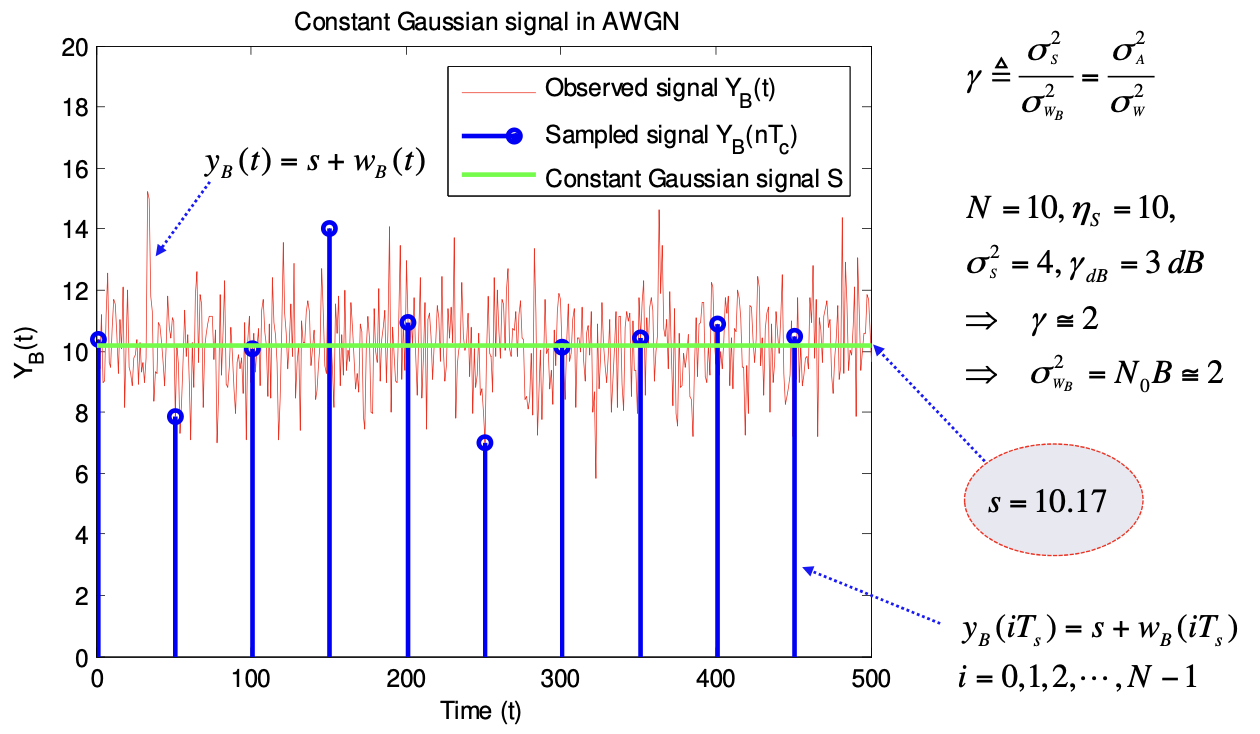
\includegraphics[width=0.65\linewidth]{Image/pdf 7/5.Const_Gauss.png}
    \label{fig:placeholder}
\end{figure}
\item Note that we do not want to estimate mean and variance of \(S\), but the value assumed by \(S\) in the specific realization we observe.
\begin{figure}[H]
    \centering
    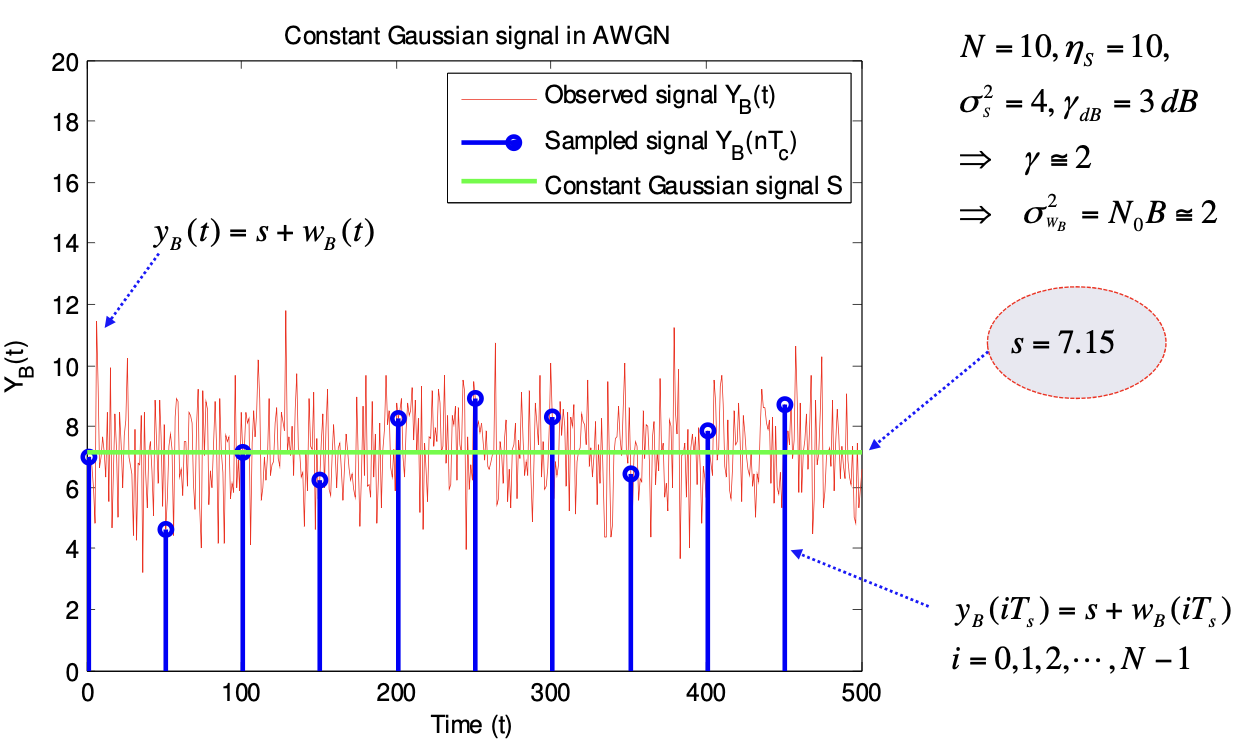
\includegraphics[width=0.65\linewidth]{Image/pdf 7/6.YB.png}
    \label{fig:placeholder}
\end{figure}
\item In the previous realization \(s=10.17\) and in this one \(s=7.15\).
\begin{figure}[H]
    \centering
    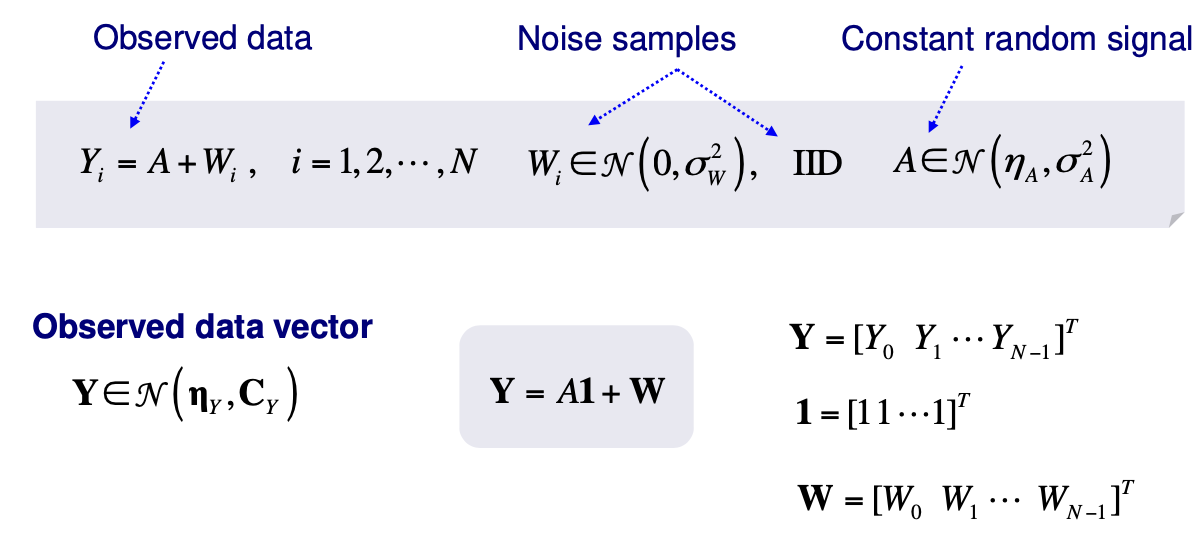
\includegraphics[width=0.65\linewidth]{Image/pdf 7/7.Data.png}
    \label{fig:placeholder}
\end{figure}
\item Let us concentrate on the estimate of \(A\)(once we have the estimate of \(A\), the estimate of \(S\) is immediately obtained:
\[
\hat{S}_{MMSE}=\sqrt{2B}\cdot\hat{A}_{MMSE}
\]
\item The signal vector \textbf{S} is a particular case of the Gaussian linear model for \(p=1\):
$$\mathbf{S} = \mathbf{H}\boldsymbol{\theta} = \mathbf{A}\mathbf{1} \quad \rightarrow \quad \mathbf{H}=1, \quad \boldsymbol{\theta}=A$$
\item Let us derive the \textbf{ML} and \textbf{MMSE} estimators by using previous results for the deterministic and Gaussian linear model, respectively:
$$\boldsymbol{\theta} = A, \quad \boldsymbol{\eta}_{\boldsymbol{\theta}} = \eta_{A}, \quad \mathbf{C}_{\boldsymbol{\theta}} = \sigma_{A}^{2}, \quad \mathbf{H} = \mathbf{1}, \quad \mathbf{C}_{\mathbf{W}} = \sigma_{W}^{2} \mathbf{I}$$
\item The \textbf{ML} estimator of \(S\), i.e. the estimator that we derived under the assumption that \(A\) is deterministic (so which does not use the \textit{a-priori} odf, but \underline{only} the observed data vector \textbf{Y}) is given by the \textbf{Sample mean}, in fact:
\begin{align*}
&\hat{A}_{ML} = \left(\mathbf{H}^{T} \mathbf{C}_{\mathbf{W}}^{-1} \mathbf{H}\right)^{-1} \mathbf{H}^{T} \mathbf{C}_{\mathbf{W}}^{-1} \mathbf{Y} = \left(\frac{1}{\sigma_{W}^{2}} \mathbf{1}^{T} \mathbf{1}\right)^{-1} \frac{1}{\sigma_{W}^{2}} \mathbf{1}^{T} \mathbf{Y} = \frac{1}{N} \mathbf{1}^{T} \mathbf{Y} = \frac{1}{N} \sum_{i=0}^{N-1} Y_{i} \\[1em]
&E\left\{A - \hat{A}_{ML}\right\} = \eta_{A} - \frac{1}{N} \mathbf{1}^{T} E\{\mathbf{Y}\} = \eta_{A} - \frac{1}{N} \mathbf{1}^{T} (\eta_{A}\mathbf{1}) = \eta_{A} - \eta_{A} = 0 \\[1em]
&MSE\left\{\hat{A}_{ML}\right\} = E\left\{(A - \hat{A}_{ML})^{2}\right\} = \left(\mathbf{H}^{T} \mathbf{C}_{\mathbf{W}}^{-1} \mathbf{H}\right)^{-1} = \left(\frac{1}{\sigma_{W}^{2}} \mathbf{1}^{T} \mathbf{1}\right)^{-1} = \left(\frac{N}{\sigma_{W}^{2}}\right)^{-1} = \frac{\sigma_{W}^{2}}{N}
\end{align*}
\item The ML estimator is linear, Gaussian distributed, unbiased, efficient and consistent.

\item \underline{The MSE when \(A\) is random} can be derived as follows\(\mathbf{Y}=A\mathbf{1}+\mathbf{W}\):

\begin{align*}
MSE\{\hat{A}_{ML}\} &= E\{(A - \hat{A}_{ML})^{2}\} = E\left\{\left(A - \frac{1}{N} \mathbf{1}^{T} \mathbf{Y}\right)^{2}\right\} = E\left\{\left(A - \frac{A}{N} \mathbf{1}^{T} \mathbf{1} - \frac{1}{N} \mathbf{1}^{T} \mathbf{W}\right)^{2}\right\} \\
&= E\left\{\left(-\frac{1}{N} \mathbf{1}^{T} \mathbf{W}\right)^{2}\right\} = \frac{1}{N^{2}} E\left\{(\mathbf{1}^{T} \mathbf{W})(\mathbf{1}^{T} \mathbf{W})^{T}\right\} = \frac{1}{N^{2}} \mathbf{1}^{T} E\{\mathbf{W}\mathbf{W}^{T}\}\mathbf{1} \\
&= \frac{\sigma_{W}^{2}}{N^{2}} \mathbf{1}^{T} \mathbf{1} = \frac{\sigma_{W}^{2}}{N}
\end{align*}

\item Which is the same as that we derived under the assumption that \(A\) is a deterministic parameter:
\begin{align*}
MSE\{\hat{A}_{ML}\}|_{A \text{ det}} &= CRB(A)|_{A \text{ det}} = \left(\mathbf{H}^{T} \mathbf{C}_{\mathbf{W}}^{-1} \mathbf{H}\right)^{-1} = \frac{\sigma_{W}^{2}}{N}
\end{align*}
\item Now let us derive the \textbf{MMSE estimator} of \(A\), i.e. the optimal estimator which makes use of both the \textit{a-priori} information (the \textit{a-priori} pdf) and the \(N\) observed data \textbf{Y}, by exploiting results for the \textbf{Gaussian linear model}.
$$\boxed{\boldsymbol{\theta} = A, \quad \boldsymbol{\eta}_{\boldsymbol{\theta}} = \eta_{A}, \quad \mathbf{C}_{\boldsymbol{\theta}} = \sigma_{A}^{2}, \quad \mathbf{H} = \mathbf{1}, \quad \mathbf{C}_{\mathbf{W}} = \sigma_{W}^{2} \mathbf{I}}$$
\vspace{-1.5em}
\begin{align*}
\hat{A}_{MMSE} &= \boldsymbol{\eta}_{A} + \left(\mathbf{C}_{A}^{-1} + \mathbf{H}^{T} \mathbf{C}_{\mathbf{W}}^{-1} \mathbf{H}\right)^{-1} \mathbf{H}^{T} \mathbf{C}_{\mathbf{W}}^{-1} (\mathbf{Y} - \mathbf{H} \boldsymbol{\eta}_{A}) \\[6pt]
&= \eta_{A} + \left(\frac{1}{\sigma_{A}^{2}} + \frac{N}{\sigma_{W}^{2}}\right)^{-1} \frac{1}{\sigma_{W}^{2}} \mathbf{1}^{T} (\mathbf{Y} - \mathbf{1}\eta_{A}) = \eta_{A} + \left(\frac{\sigma_{W}^{2} + N\sigma_{A}^{2}}{\sigma_{A}^{2} \sigma_{W}^{2}}\right)^{-1} \frac{1}{\sigma_{W}^{2}} \mathbf{1}^{T} (\mathbf{Y} - \mathbf{1}\eta_{A}) \\[6pt]
&= \eta_{A} + \frac{\sigma_{A}^{2}}{\sigma_{W}^{2} + N\sigma_{A}^{2}} (\mathbf{1}^{T} \mathbf{Y} - N\eta_{A}) = \frac{\sigma_{A}^{2}}{\sigma_{W}^{2} + N\sigma_{A}^{2}} \mathbf{1}^{T} \mathbf{Y} + \left(1 - \frac{N\sigma_{A}^{2}}{\sigma_{W}^{2} + N\sigma_{A}^{2}}\right)\eta_{A}
\end{align*}
\item We can derive:
\begin{align*}
\hat{A}_{MMSE} &= \frac{\sigma_{A}^{2}}{\sigma_{W}^{2} + N\sigma_{A}^{2}} \mathbf{1}^{T} \mathbf{Y} + \left(1 - \frac{N\sigma_{A}^{2}}{\sigma_{W}^{2} + N\sigma_{A}^{2}}\right)\eta_{A} = \frac{N\sigma_{A}^{2}}{\sigma_{W}^{2} + N\sigma_{A}^{2}} \cdot \frac{1}{N} \mathbf{1}^{T} \mathbf{Y} + \frac{\sigma_{W}^{2}}{\sigma_{W}^{2} + N\sigma_{A}^{2}}\eta_{A} \\[1em]
&= \alpha \cdot \frac{1}{N} \mathbf{1}^{T} \mathbf{Y} + (1-\alpha)\eta_{A} = \alpha\hat{A}_{ML} + (1-\alpha)\hat{A}_{ap}
\end{align*}
\item Where we defined:
$$\boxed{\alpha \triangleq \frac{N\sigma_{A}^{2}}{\sigma_{W}^{2} + N\sigma_{A}^{2}} = \frac{N\gamma}{1 + N\gamma} = \frac{PG \cdot \gamma}{1 + PG \cdot \gamma} \in [0,1], \quad \gamma \triangleq \frac{\sigma_{A}^{2}}{\sigma_{W}^{2}} \in [0, +\infty)}$$
\item We study the MSE:
\begin{align*}
MSE\{\hat{A}_{MMSE}\} &= \left(\mathbf{C}_{\boldsymbol{\theta}}^{-1} + \mathbf{H}^{T} \mathbf{C}_{\mathbf{W}}^{-1} \mathbf{H}\right)^{-1} \\[6pt]
&= \left(\frac{1}{\sigma_{A}^{2}} + \frac{N}{\sigma_{W}^{2}}\right)^{-1} = \left(\frac{\sigma_{W}^{2} + N\sigma_{A}^{2}}{\sigma_{A}^{2} \sigma_{W}^{2}}\right)^{-1} \\[6pt]
&= \frac{\sigma_{A}^{2}\sigma_{W}^{2}}{\sigma_{W}^{2} + N\sigma_{A}^{2}} = \left(1 - \frac{N\sigma_{A}^{2}}{\sigma_{W}^{2} + N\sigma_{A}^{2}}\right)\sigma_{A}^{2} = (1-\alpha)\sigma_{A}^{2} = (1-\alpha)\cdot MSE\{\hat{A}_{ap}\} \\[6pt]
&= \frac{\sigma_{A}^{2}\sigma_{W}^{2}}{\sigma_{W}^{2} + N\sigma_{A}^{2}} = \frac{N\sigma_{A}^{2}}{\sigma_{W}^{2} + N\sigma_{A}^{2}} \cdot \frac{\sigma_{W}^{2}}{N} = \alpha \cdot \frac{\sigma_{W}^{2}}{N} = \alpha \cdot MSE\{\hat{A}_{ML}\}
\end{align*}
\item In summary:
\[
\boxed{\begin{cases}
\hat{A}_{ap} = \eta_{A} \\[8pt]
\hat{A}_{ML} = \frac{1}{N} \mathbf{1}^{T} \mathbf{Y} \\[8pt]
\hat{A}_{MMSE} = \alpha \hat{A}_{ML} + (1-\alpha) \hat{A}_{ap}
\end{cases}}
\]
\item And also:
\[
MSE\{\hat{A}_{ap}\} = \sigma_{A}^{2} \quad
MSE\{\hat{A}_{ML}\} = \frac{\sigma_{W}^{2}}{N} \quad
MSE\{\hat{A}_{MMSE}\} = \frac{\sigma_{W}^{2}}{N} = (1-\alpha)\sigma_{A}^{2}
\]
\[
\alpha = \frac{N\gamma}{1+N\gamma} \in [0,1) \implies
\begin{cases}
MSE\{\hat{A}_{MMSE}\} = (1-\alpha) \cdot MSE\{\hat{A}_{ap}\} \leq MSE\{\hat{A}_{ap}\} \\[10pt]
MSE\{\hat{A}_{MMSE}\} = \alpha \cdot MSE\{\hat{A}_{ML}\} \leq MSE\{\hat{A}_{ML}\}
\end{cases}
\]
\item All the three estimators are \textbf{linear},\textbf{Gaussian distributed}, and \textbf{unbiased}:
\begin{figure}[H]
    \centering
    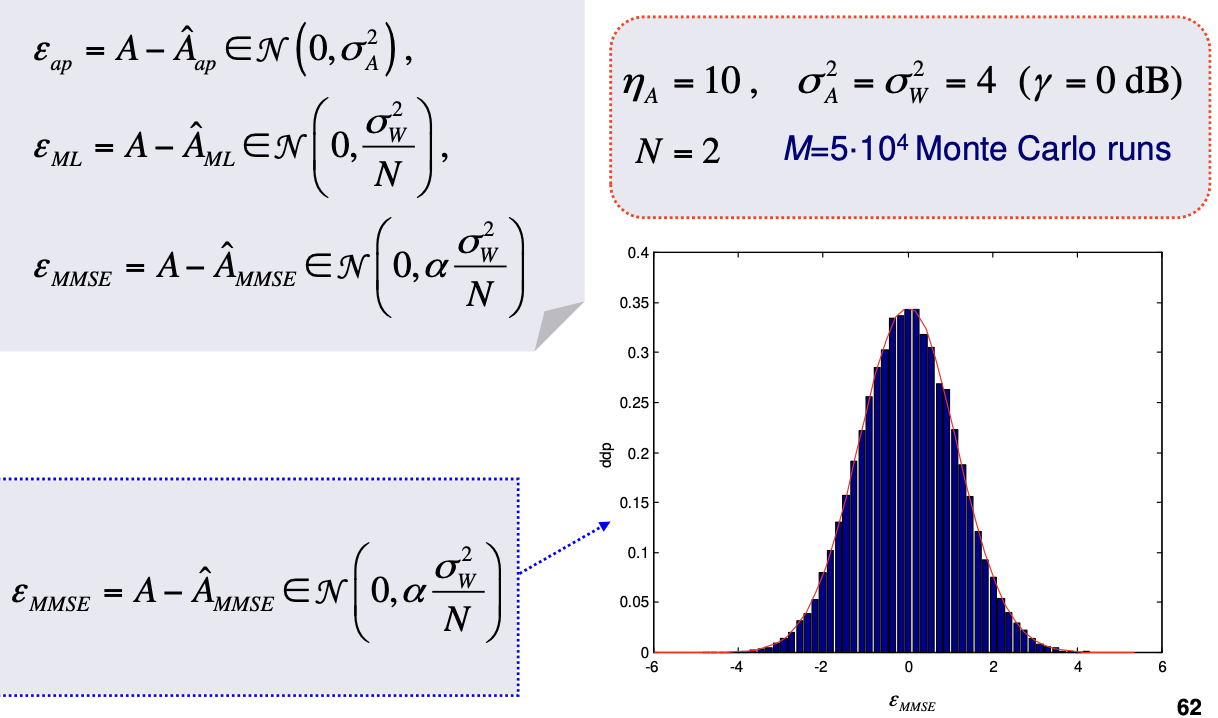
\includegraphics[width=0.65\linewidth]{Image/pdf 7/8.Resume.png}
    \label{fig:placeholder}
\end{figure}

\item The MSE's of the three estimators do not depend on the mean value of \(A\) but only on its variance and/or the noise variance.
\item Coefficient \(\alpha\) represents the improvement in terms of MSE of the MMSE estimator w.r.t. the ML estimator, achieved by properly exploiting the knowledge of the \textit{a-priori} pdf of \(A\). The ML estimator uses only the observed data, the MMSE uses the observed data and the \textit{a-priori} information.
\item The ML and MMSE estimators coincide when \(\alpha\) tends to 1, i.e. when \(N\) and/or \(\gamma\) tend to infinity.
\item Coefficient \(1-\alpha\) represents the improvement in terms of MSE of the MMSE estimator w.r.t. the \textit{A-posteriori} estimator, achieved by properly exploiting the observed data, in addition to the \textit{a-priori} information. The \textit{A-priori} estimator uses only the knowledge of the \textit{a-priori} pdf of \(A\), but not observed data. The MMSE uses observed data and \textit{a-priori} information.
\item The \textit{A-priori} and MMSE estimators coincide when \(\alpha\) tends to 0, i.e. when \(N\) and/or \(\gamma\) tend to 0.
\begin{figure}[H]
    \centering
    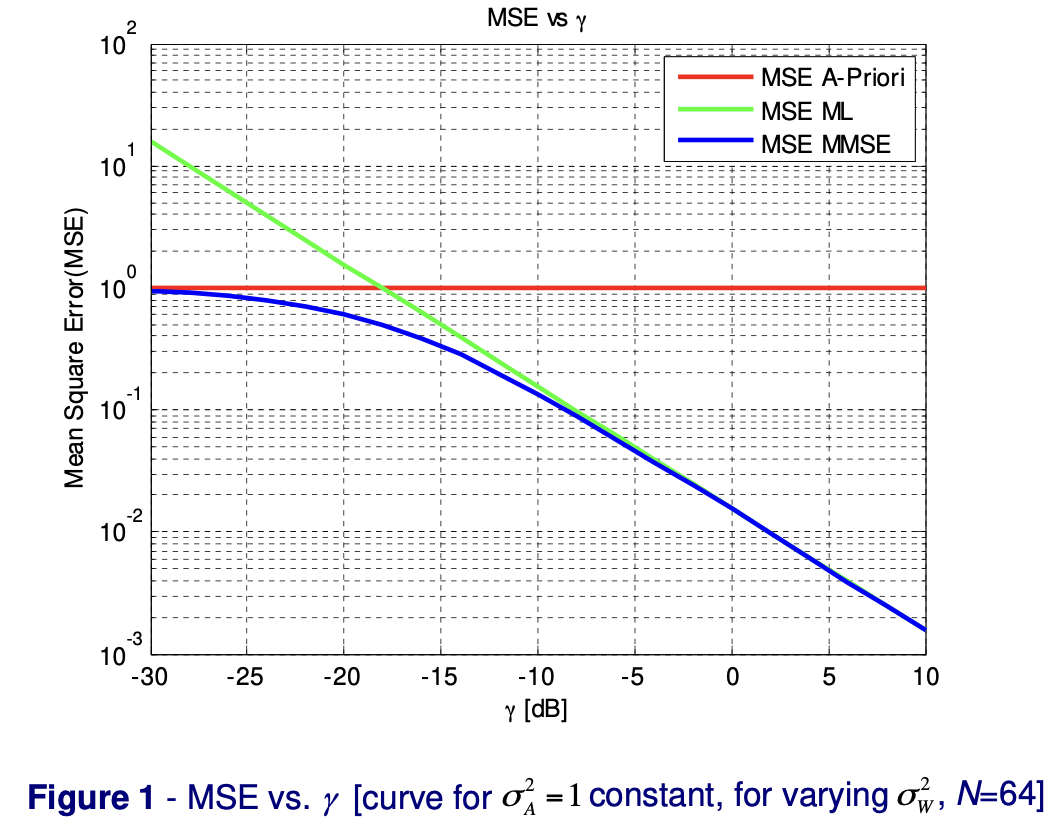
\includegraphics[width=0.65\linewidth]{Image/pdf 7/9.MSE_vs_y.png}
    \label{fig:placeholder}
\end{figure}
\begin{figure}[H]
    \centering
    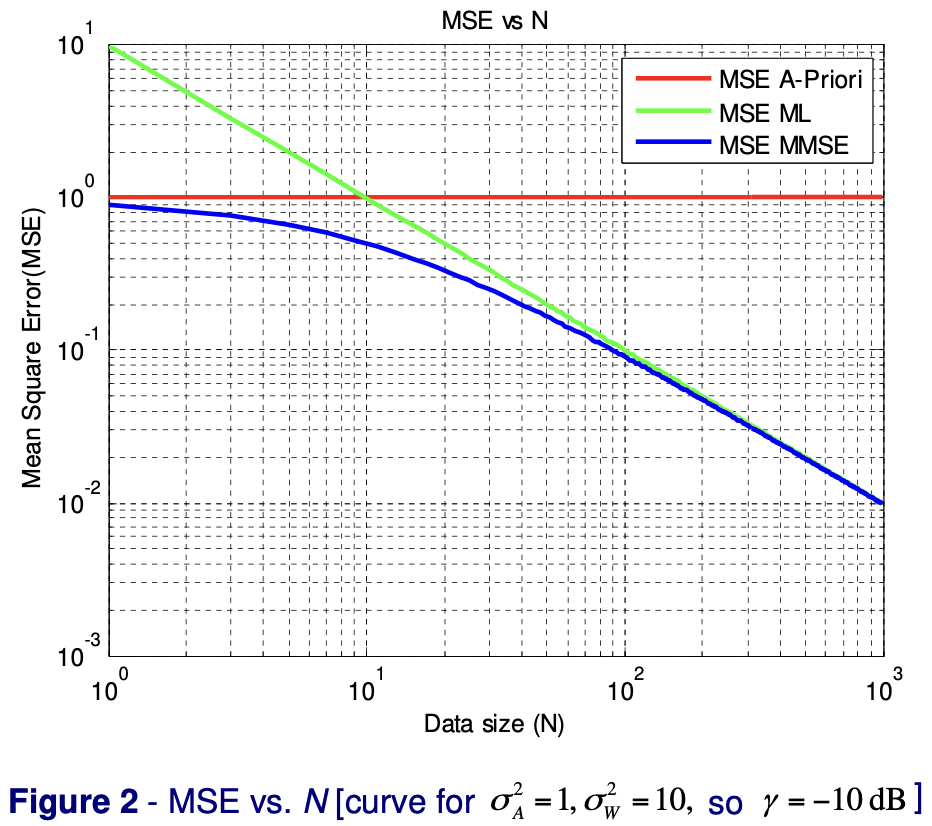
\includegraphics[width=0.55\linewidth]{Image/pdf 7/10.MSE_vs_y_2.png}
    \label{fig:placeholder}
\end{figure}
\item \textbf{Example}: Let us consider again the \textbf{problem of estimating amplitude and phase of a sinusoid in AWGN}:
\begin{align*}
X_{k} &= \frac{1}{\sqrt{2B}} X_{B}\left(\frac{k}{2B}\right) = \frac{A}{\sqrt{2B}} \cos \left(2\pi f_{0} \frac{k}{2B} + \theta\right) + \frac{1}{\sqrt{2B}} W_{B}\left(\frac{k}{2B}\right), \quad 0 \le k \le N-1 \\
&= \frac{A}{\sqrt{2B}}\cos(\theta)\cos\left(2\pi F_{0}k\right) - \frac{A}{\sqrt{2B}}\sin(\theta)\sin\left(2\pi F_{0}k\right) + W_{k}, \quad \text{where } F_{0} \triangleq \frac{f_{0}}{2B}
\end{align*}
$$
\begin{cases}
\theta_{1} \triangleq \frac{A}{\sqrt{2B}}\cos(\theta) & \left\{ \mathbf{h}_{1} \triangleq \begin{bmatrix} 1 & \cos(2\pi F_{0}) & \cdots & \cos(2\pi F_{0}(N-1)) \end{bmatrix}^{T} \right. \\
\theta_{2} \triangleq -\frac{A}{\sqrt{2B}}\sin(\theta) & \left. \mathbf{h}_{2} \triangleq \begin{bmatrix} 0 & \sin(2\pi F_{0}) & \cdots & \sin(2\pi F_{0}(N-1)) \end{bmatrix}^{T} \right.
\end{cases}
$$
$$
\Downarrow
$$
$$\mathbf{X} = A\mathbf{p}(\theta) = \theta_{1}\mathbf{h}_{1} + \theta_{2}\mathbf{h}_{2} + \mathbf{W} = \mathbf{H}\boldsymbol{\theta} + \mathbf{W}$$
\end{itemize}
\subsection{Linear Models}
\subsubsection{Deterministic Linear Model}
\begin{itemize}
\item Thanks to a proper re-parametrization of the SOI, we obtained the so-called \textbf{Deterministic Linear Model}:
$$\underset{2 \times 1}{\boldsymbol{\theta}} = \begin{bmatrix} \theta_{1} \\ \theta_{2} \end{bmatrix}, \quad \underset{N \times 2}{\mathbf{H}} = [\mathbf{h}_{1} \quad \mathbf{h}_{2}] \quad \Rightarrow \quad \mathbf{X} = \mathbf{H}\boldsymbol{\theta} + \mathbf{W}$$
\item If we assume that \(W(t)\) is AWGN with Power Spectral Density (PSD) equal to \(N_0/2\), we get:
$$\mathbf{W} \in \mathcal{N}(\mathbf{0}, \sigma_{W}^{2}\mathbf{I}), \quad \text{where } \sigma_{W}^{2} = \frac{N_{0}}{2}$$
\item Under these assumptions, we found that the \textbf{ML estimator} coincides with the \textbf{Linear Least Squares (LS) estimator}.

\item \textbf{ML estimator = Linear LS estimator} \(\rightarrow\) it is \textbf{linear},\textbf{unbiased}, \textbf{Gaussian distributed},\textbf{efficient}, and \textbf{consistent}:
\begin{align*}
&\hat{\boldsymbol{\theta}}_{ML} = \hat{\boldsymbol{\theta}}_{LS} = \mathbf{H}^{\#}\mathbf{X} = (\mathbf{H}^{H}\mathbf{H})^{-1}\mathbf{H}^{H}\mathbf{X} \\[1em]
&E\left\{\hat{\boldsymbol{\theta}}_{ML}\right\} = \boldsymbol{\theta}, \quad MSE\left\{\hat{\boldsymbol{\theta}}_{ML}\right\} = CRB(\boldsymbol{\theta}) = \sigma_{W}^{2}(\mathbf{H}^{H}\mathbf{H})^{-1} \\[1em]
&\hat{\boldsymbol{\theta}}_{ML} \in \mathcal{N}(\boldsymbol{\theta}, CRB(\boldsymbol{\theta}))
\end{align*}
\item Taking into account that sine and cosine at the same frequency are orthogonal and that the energy of the two vectors \textbf{h}, is equal to \(N/2\), we found that:
$$\mathbf{H}^{T}\mathbf{H} \cong \frac{N}{2}\mathbf{I} \quad \text{if } N = 2BT \gg 1$$



\item The ML estimates of \(\theta_1\) and \(\theta_2\) and their MSE's were derived to be:
\begin{align*}
&\hat{\boldsymbol{\theta}}_{ML} = (\mathbf{H}^{T}\mathbf{H})^{-1}\mathbf{H}^{T}\mathbf{X} \cong \left(\frac{N}{2}\mathbf{I}\right)^{-1}\begin{bmatrix} \mathbf{h}_{1}^{T}\mathbf{X} \\ \mathbf{h}_{2}^{T}\mathbf{X} \end{bmatrix} = \frac{2}{N}\begin{bmatrix} \mathbf{h}_{1}^{T}\mathbf{X} \\ \mathbf{h}_{2}^{T}\mathbf{X} \end{bmatrix} \\[1em]
&\hat{\theta}_{1,ML} = \frac{2}{N}\sum_{n=0}^{N-1} X_{n}\cos(2\pi F_{0}n) \qquad\hat{\theta}_{2,ML} = \frac{2}{N}\sum_{n=0}^{N-1} X_{n}\sin(2\pi F_{0}n) \\[1em]
&MSE\{\hat{\theta}_{k,ML}\} = CRB(\theta_{k}) = \frac{2\sigma_{W}^{2}}{N}, \quad k=1,2
\end{align*}

\item The ML estimate of \(A\) and \(\theta\) is immediately derived once we have the ML estimate of vector \(\theta\), thanks to the \textbf{invariance property} of the ML estimate:
\[
\hat{\boldsymbol{\theta}}_{ML}=\begin{bmatrix}
    \hat{\theta}_{1,ML}\\[4pt]
    \hat{\theta}_{2,ML}
\end{bmatrix}=\mathbf{H}^{\#}\mathbf{X}
\]
\[
\Downarrow
\]\[
\begin{cases}
A = \sqrt{2B} \sqrt{\theta_{1}^{2} + \theta_{2}^{2}} & \\
\theta = -\text{Arctg} \left(\frac{\theta_{2}}{\theta_{1}}\right)
\end{cases}
\Rightarrow
\begin{cases}
\hat{A}_{ML} = \sqrt{2B} \sqrt{\hat{\theta}_{1,ML}^{2} + \hat{\theta}_{2,ML}^{2}} \\
\hat{\theta}_{ML} = -\text{Arctg} \left(\frac{\hat{\theta}_{2,ML}}{\hat{\theta}_{1,ML}}\right)
\end{cases}\]
\end{itemize}
\subsubsection{Bayesian Linear Model: MMSE estimate}
\begin{itemize}
    \item \textbf{Assumption}: The amplitude \(A\) is random, e.g. due to propagation effects on a random channel, and can be modelled as a Rayleigh r.v. (in this case we talk about "Rayleigh channel"). Whereas, the phase \(\theta\) is typically modelled as a r.v. uniformly distributed \([-\pi,\pi)\). Amplitude and phase can be assumed to be independent.
 \[   \begin{cases}
A \in \mathcal{R}(\sigma_{A}^{2}) & \Theta \in \mathcal{U}(-\pi, \pi) \\
f_{A}(a) = \frac{a}{\sigma_{A}^{2}} e^{-\frac{a^{2}}{2\sigma_{A}^{2}}}u(a), & \text{with } E\{A^{2}\} = 2\sigma_{A}^{2}
\end{cases}\]

\[
\text{Data model: } \mathbf{X} = A\mathbf{p}(\theta) + \mathbf{W} = \theta_{1}\mathbf{h}_{1} + \theta_{2}\mathbf{h}_{2} + \mathbf{W} = \mathbf{H}\boldsymbol{\theta} + \mathbf{W} \]
\[
\boldsymbol{\theta} = \begin{bmatrix} \theta_{1} \\ \theta_{2} \end{bmatrix} \triangleq \begin{bmatrix} \frac{A}{\sqrt{2B}}\cos(\theta) \\ -\frac{A}{\sqrt{2B}}\sin(\theta) \end{bmatrix}
\]

\item It is basically a transformation from Polar coordinates to Cartesian coordinates.
\item To find the joint pdf of \(\theta_1\) and \(\theta_2\) we should apply \textbf{the Fundamental Theorem} for the transformation of random vectors.
\item Since \(A>0\), the system of equations has a unique solution:
\[\begin{cases}
A = \sqrt{2B} \sqrt{\theta_{1}^{2} + \theta_{2}^{2}} \\
\theta = -\text{arctg} \left(\frac{\theta_{2}}{\theta_{1}}\right)
\end{cases}
\longleftarrow \text{atan2}(-\theta_{2}, \theta_{1})\]\vspace{-1em}
\begin{gather*}
f_{\theta_{1},\theta_{2}}(\theta_{1}, \theta_{2}) = \frac{f_{A,\theta}(a,\theta)}{|\mathbf{J}|} \Bigg|_{\substack{a=\sqrt{2B}\sqrt{\theta_{1}^{2}+\theta_{2}^{2}} \\ \theta=-\text{Arctg}(\theta_{2}/\theta_{1})}} = \frac{1}{|\mathbf{J}|} \cdot \frac{a}{\sigma_{A}^{2}} e^{-\frac{a^{2}}{2\sigma_{A}^{2}}}u(a) \cdot \frac{1}{2\pi}\text{rect}\left(\frac{\theta}{2\pi}\right) \Bigg|_{\substack{a=\sqrt{2B}\sqrt{\theta_{1}^{2}+\theta_{2}^{2}} \\ \theta=-\text{Arctg}(\theta_{2}/\theta_{1})}}
\end{gather*}
\item \textbf{J} is the Jacobian of the transformation:
\begin{align*}
\mathbf{J} = \begin{vmatrix}
\frac{\partial \theta_{1}}{\partial a} & \frac{\partial \theta_{1}}{\partial \theta} \\
\frac{\partial \theta_{2}}{\partial a} & \frac{\partial \theta_{2}}{\partial \theta}
\end{vmatrix} &= \begin{vmatrix}
\frac{1}{\sqrt{2B}} \cos \theta & - \frac{a}{\sqrt{2B}} \sin \theta \\
- \frac{1}{\sqrt{2B}} \sin \theta & - \frac{a}{\sqrt{2B}} \cos \theta
\end{vmatrix} = - \frac{a}{2B} \cos^{2} \theta - \frac{a}{2B} \sin^{2} \theta = - \frac{a}{2B}  \\[2em]
f_{\theta_{1},\theta_{2}}(\theta_{1}, \theta_{2}) &= \frac{1}{|\mathbf{J}|} \cdot f_{A,\theta}(a,\theta) \Bigg|_{\substack{a=\sqrt{2B}\sqrt{\theta_{1}^{2}+\theta_{2}^{2}} \\ \theta=-\text{Arctg}(\theta_{2}/\theta_{1})}} = \frac{1}{|\mathbf{J}|} \cdot \frac{a}{\sigma_{A}^{2}} e^{-\frac{a^{2}}{2\sigma_{A}^{2}}}u(a) \cdot \frac{1}{2\pi}\text{rect}\left(\frac{\theta}{2\pi}\right) \Bigg|_{\substack{a=\sqrt{2B}\sqrt{\theta_{1}^{2}+\theta_{2}^{2}} \\ \theta=-\text{Arctg}(\theta_{2}/\theta_{1})}} \\[1em]
&= \frac{2B}{a} \cdot \frac{a}{2\pi \sigma_{A}^{2}} e^{-\frac{a^{2}}{2\sigma_{A}^{2}}}u(a) \cdot \text{rect}\left(\frac{\theta}{2\pi}\right) \Bigg|_{\substack{a=\sqrt{2B}\sqrt{\theta_{1}^{2}+\theta_{2}^{2}} \\ \theta=-\text{Arctg}(\theta_{2}/\theta_{1})}}
\end{align*}
\item The joint pdf of \(\theta_1\) and \(\theta_2\) is finally obtained:
\begin{align*}
f_{\theta_{1},\theta_{2}}(\theta_{1}, \theta_{2}) = \frac{2B}{2\pi \sigma_{A}^{2}} e^{-\frac{2B}{2\sigma_{A}^{2}}(\theta_{1}^{2}+\theta_{2}^{2})} \cdot u(a) \cdot \text{rect}\left(\frac{\theta}{2\pi}\right) =\frac{2B}{2\pi\sigma_A^2}e^{\frac{-2B(\theta_1^2+\theta_2^2)}{2\sigma_{A}^2}}\\
= \frac{1}{\sqrt{2\pi \frac{\sigma_{A}^{2}}{2B}}} e^{-\frac{\theta_{1}^{2}}{2\frac{\sigma_{A}^{2}}{2B}}} \cdot \frac{1}{\sqrt{2\pi \frac{\sigma_{A}^{2}}{2B}}} e^{-\frac{\theta_{2}^{2}}{2\frac{\sigma_{A}^{2}}{2B}}} = f_{\theta_{1}}(\theta_{1}) f_{\theta_{2}}(\theta_{2})
\end{align*}
\[
\theta_{1} \in \mathcal{N}\left(0, \frac{\sigma_{A}^{2}}{2B}\right), \quad \theta_{2} \in \mathcal{N}\left(0, \frac{\sigma_{A}^{2}}{2B}\right), \quad \text{IID}
\]
\end{itemize}
\subsubsection{Gaussian Linear Model: MMSE estimate}
\begin{itemize}
\item Hence, the SOI can be modelled by the \underline{\textbf{Gaussian linear model}}:
\begin{align*}
&\mathbf{X} = \mathbf{H}\boldsymbol{\theta} + \mathbf{W} \\
&\boldsymbol{\theta}\in\mathcal{N}(\boldsymbol{\eta}_{\boldsymbol{\theta}}, \mathbf{C}_{\boldsymbol{\theta}}), \quad \boldsymbol{\eta}_{\boldsymbol{\theta}} = \begin{bmatrix} 0 \\ 0 \end{bmatrix}, \quad \mathbf{C}_{\boldsymbol{\theta}} = \sigma_{\theta}^{2}\mathbf{I} = \frac{\sigma_{A}^{2}}{2B}\mathbf{I} \\
&\mathbf{W}\in\mathcal{N}(\mathbf{0}, \mathbf{C}_{\mathbf{W}}), \quad \text{where } \mathbf{C}_{\mathbf{W}} = \sigma_{W}^{2}\mathbf{I} \text{ and } \sigma_{W}^{2} = \frac{N_{0}}{2} \\
&\mathbf{H} = [\mathbf{h}_{1} \quad \mathbf{h}_{2}], \quad
\begin{cases}
\mathbf{h}_{1} = \begin{bmatrix} 1 & \cos(2\pi F_{0}) & \cdots & \cos(2\pi F_{0}(N-1)) \end{bmatrix}^{T} \\
\mathbf{h}_{2} = \begin{bmatrix} 0 & \sin(2\pi F_{0}) & \cdots & \sin(2\pi F_{0}(N-1)) \end{bmatrix}^{T}
\end{cases}
\end{align*}
\item extbf{Problem}: find the MMSE estimator of the Gaussian random vector \(\theta\) given the observed data vector \textbf{X}(under the assumption) that \(F_0\) is known.
\item The general expression of the \textbf{MMSE estimator} of the Gaussian random vector and of the covariance matrix of the estimation errors (i. the MSE matrix) have already been derived:

\begin{align*}
&\mathbf{\hat{\boldsymbol{\theta}}}_{\text{MMSE}} = \boldsymbol{\eta}_{\boldsymbol{\theta}} + \left(\mathbf{C}_{\boldsymbol{\theta}}^{-1} + \mathbf{H}^{T}\mathbf{C}_{\mathbf{W}}^{-1}\mathbf{H}\right)^{-1}\mathbf{H}^{T}\mathbf{C}_{\mathbf{W}}^{-1} \left(\mathbf{X} - \mathbf{H}\boldsymbol{\eta}_{\boldsymbol{\theta}}\right) \\
&\text{MSE}\left\{\mathbf{\hat{\boldsymbol{\theta}}}_{\text{MMSE}}\right\} = \mathbf{C}_{\boldsymbol{\theta}|\mathbf{X}} = \left(\mathbf{C}_{\boldsymbol{\theta}}^{-1} + \mathbf{H}^{T}\mathbf{C}_{\mathbf{W}}^{-1}\mathbf{H}\right)^{-1} = \text{BCRB}(\boldsymbol{\theta}) \\
\end{align*}
\item We can rewrite it:

\begin{align*}
&\mathbf{\hat{\boldsymbol{\theta}}}_{\text{MMSE}} = \frac{1}{\sigma_{W}^{2}}\left(\frac{1}{\sigma_{\theta}^{2}}\mathbf{I} + \frac{1}{\sigma_{W}^{2}}\mathbf{H}^{T}\mathbf{H}\right)^{-1}\mathbf{H}^{T}\mathbf{X} \\
&\text{MSE}\left\{\mathbf{\hat{\boldsymbol{\theta}}}_{\text{MMSE}}\right\} = \left(\frac{1}{\sigma_{\theta}^{2}}\mathbf{I} + \frac{1}{\sigma_{W}^{2}}\mathbf{H}^{T}\mathbf{H}\right)^{-1},\qquad \text{where} \quad\sigma_{\theta}^2=\frac{\sigma_A^2}{2B}, \quad\sigma_W^2=\frac{N_0}{2}
\end{align*}
\item \textbf{H} is:
$$
\mathbf{H} = [\mathbf{h}_{1} \quad \mathbf{h}_{2}], \quad
\begin{cases}
\mathbf{h}_{1} = \begin{bmatrix} 1 & \cos(2\pi F_{0}) & \cdots & \cos(2\pi F_{0}(N-1)) \end{bmatrix}^{T} \\
\mathbf{h}_{2} = \begin{bmatrix} 0 & \sin(2\pi F_{0}) & \cdots & \sin(2\pi F_{0}(N-1)) \end{bmatrix}^{T}
\end{cases}
$$
\item Recalling that: \[
\mathbf{H^T}\mathbf{H}\approx \frac{N}{2}\textbf{I},\text{ if }N=2BT\gg1
\]
\item We find:
\begin{align*}
&\mathbf{\hat{\boldsymbol{\theta}}}_{\text{MMSE}} = \frac{1}{\sigma_{W}^{2}}\left(\frac{1}{\sigma_{\theta}^{2}}\mathbf{I} + \frac{N}{2\sigma_{W}^{2}}\mathbf{I}\right)^{-1} \begin{bmatrix} \mathbf{h}_{1}^{T}\mathbf{X} \\ \mathbf{h}_{2}^{T}\mathbf{X} \end{bmatrix} = \frac{2\sigma_{\theta}^{2}}{2\sigma_{W}^{2} + N\sigma_{\theta}^{2}} \begin{bmatrix} \mathbf{h}_{1}^{T}\mathbf{X} \\ \mathbf{h}_{2}^{T}\mathbf{X} \end{bmatrix} \\
&\text{MSE}\left\{\mathbf{\hat{\boldsymbol{\theta}}}_{\text{MMSE}}\right\} = \frac{2\sigma_{W}^{2}\sigma_{\theta}^{2}}{2\sigma_{W}^{2} + N\sigma_{\theta}^{2}}\mathbf{I}
\end{align*}
\item In summary, the MMSE estimates of \(\theta_1\) and \(\theta_2\) and their MSE are given by:

\begin{align*}
&\mathbf{\hat{\theta}}_{1,\text{MMSE}} = \frac{2\sigma_{\theta}^{2}}{2\sigma_{W}^{2} + N\sigma_{\theta}^{2}}\mathbf{h}_{1}^{T}\mathbf{X} = \frac{N\sigma_{\theta}^{2}}{2\sigma_{W}^{2} + N\sigma_{\theta}^{2}} \cdot \frac{2}{N}\sum_{n=0}^{N-1} X_{n}\cos(2\pi F_{0}n) \\
&\mathbf{\hat{\theta}}_{2,\text{MMSE}} = \frac{2\sigma_{\theta}^{2}}{2\sigma_{W}^{2} + N\sigma_{\theta}^{2}}\mathbf{h}_{2}^{T}\mathbf{X} = \frac{N\sigma_{\theta}^{2}}{2\sigma_{W}^{2} + N\sigma_{\theta}^{2}} \cdot \frac{2}{N}\sum_{n=0}^{N-1} X_{n}\sin(2\pi F_{0}n) \\
&\text{MSE}\left\{\mathbf{\hat{\theta}}_{k,\text{MMSE}}\right\} = \frac{2\sigma_{W}^{2}\sigma_{\theta}^{2}}{2\sigma_{W}^{2} + N\sigma_{\theta}^{2}} = \frac{N\sigma_{\theta}^{2}}{2\sigma_{W}^{2} + N\sigma_{\theta}^{2}} \cdot \frac{2\sigma_{W}^{2}}{N}, \quad k=1,2
\end{align*}

\item The \textbf{MMSE} estimator for the \textbf{Gaussian linear model} in \textbf{AWGN} is \textbf{linear}, \textbf{Gaussian distributed}, \textbf{unbiased},\textbf{efficient} and \textbf{consistent}.

\item The MMSE estimates of \(\theta_1\) and \(\theta_2\) and their MSE can be expressed immediately in terms of the ML estimators and their MSE:

\begin{align*}
&\mathbf{\hat{\theta}}_{1,\text{MMSE}} = \frac{N\sigma_{\theta}^{2}}{2\sigma_{W}^{2} + N\sigma_{\theta}^{2}} \cdot \frac{2}{N}\sum_{n=0}^{N-1} X_{n}\cos(2\pi F_{0}n) = \alpha\mathbf{\hat{\theta}}_{1,\text{ML}} \\
&\mathbf{\hat{\theta}}_{2,\text{MMSE}} = \frac{N\sigma_{\theta}^{2}}{2\sigma_{W}^{2} + N\sigma_{\theta}^{2}} \cdot \frac{2}{N}\sum_{n=0}^{N-1} X_{n}\sin(2\pi F_{0}n) = \alpha\mathbf{\hat{\theta}}_{2,\text{ML}} \\
&\text{MSE}\left\{\mathbf{\hat{\theta}}_{k,\text{MMSE}}\right\} = \frac{N\sigma_{\theta}^{2}}{2\sigma_{W}^{2} + N\sigma_{\theta}^{2}} \cdot \frac{2\sigma_{W}^{2}}{N} = \alpha\text{MSE}\left(\mathbf{\hat{\theta}}_{k,\text{ML}}\right), \quad k=1,2 \\
&\text{where } \alpha \triangleq \frac{N\sigma_{\theta}^{2}}{2\sigma_{W}^{2} + N\sigma_{\theta}^{2}} = \frac{\frac{N}{2}\sigma_{\theta}^{2}}{\sigma_{W}^{2} + \frac{N}{2}\sigma_{\theta}^{2}} = \frac{\text{PG} \cdot \gamma}{1 + \text{PG} \cdot \gamma} \in [0,1], \quad \text{PG} = \frac{N}{2}
\end{align*}

\item Parameter \(\alpha\) is related to the input Signal-to-Noise power Ratio (SNR)\(\gamma\):
\begin{align*}
\mathbf{X} &= \mathbf{H}\boldsymbol{\theta} + \mathbf{W} \\
\gamma &\triangleq \frac{E\{\lVert \mathbf{H}\boldsymbol{\theta} \rVert^{2}\}}{E\{\lVert \mathbf{W} \rVert^{2}\}} = \frac{E\{(\mathbf{H}\boldsymbol{\theta})^{T}\mathbf{H}\boldsymbol{\theta}\}}{E\{\mathbf{W}^{T}\mathbf{W}\}} = \frac{E\{\boldsymbol{\theta}^{T}\mathbf{H}^{T}\mathbf{H}\boldsymbol{\theta}\}}{E\{\sum_{n=1}^{N} W_{n}^{2}\}} = \frac{\frac{N}{2}E\{\boldsymbol{\theta}^{T}\boldsymbol{\theta}\}}{E\{\sum_{n=1}^{N} W_{n}^{2}\}} \\
&= \frac{N\sigma_{\theta}^{2}}{N\sigma_{W}^{2}} = \frac{\sigma_{\theta}^{2}}{\sigma_{W}^{2}} = \frac{\sigma_{A}^{2}}{N_{0}B} \\
\alpha &= \frac{\frac{N}{2}\sigma_{\theta}^{2}}{\sigma_{W}^{2} + \frac{N}{2}\sigma_{\theta}^{2}} = \frac{\frac{N}{2}\gamma}{1 + \frac{N}{2}\gamma} = \frac{\text{PG} \cdot \gamma}{1 + \text{PG} \cdot \gamma}
\end{align*}

\item When \(\gamma\rightarrow +\infty\) or \(N\rightarrow+\infty\), \(\alpha\rightarrow1\), and so the MMSE estimator tends to coincide with the ML estimator.

\begin{figure}[H]
    \centering
    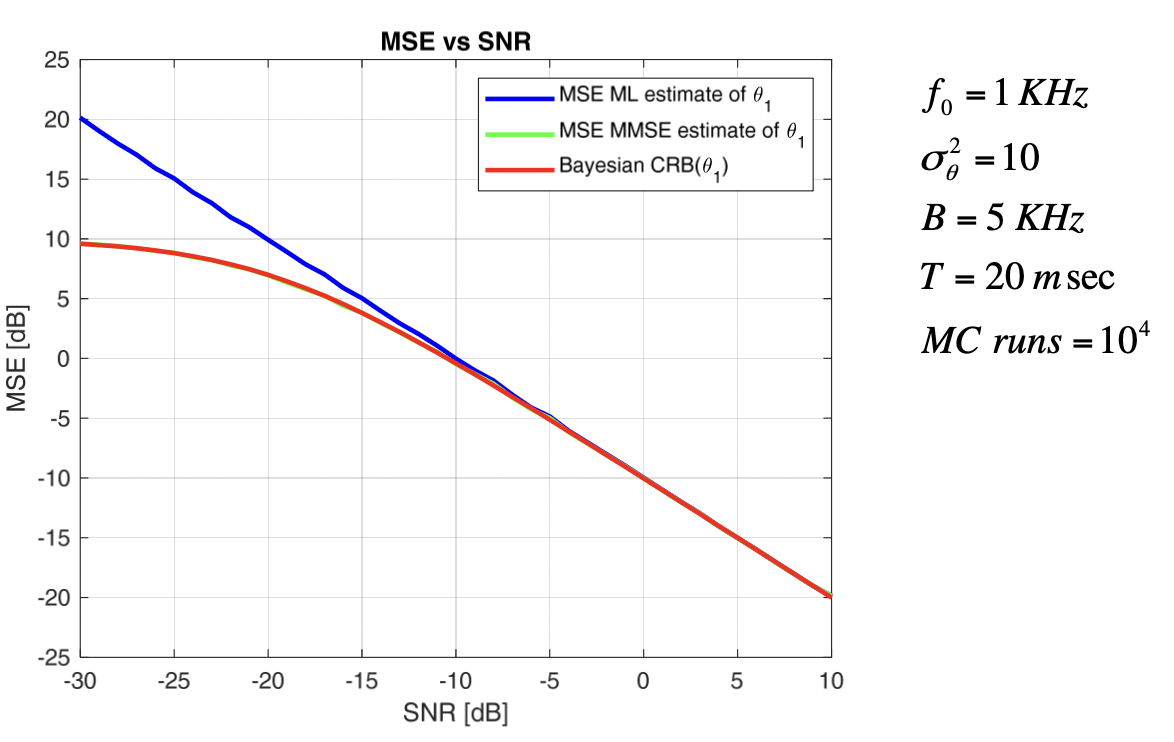
\includegraphics[width=0.65\linewidth]{Image/pdf 7/11.MSE_vs_SNR.png}
    \label{fig:placeholder}
\end{figure}

\item Once we have the MMSE estimate of \(\theta_1\) and \(\theta_2\) we can get an estimate of \(A\) and \(\theta\) as follows:
$$
\begin{cases}
\mathbf{\hat{A}} = \sqrt{2B}\sqrt{\hat{\theta}_{1,\text{MMSE}}^{2} + \hat{\theta}_{2,\text{MMSE}}^{2}} \\
\mathbf{\hat{\theta}} = -\text{arctg}\left(\hat{\theta}_{2,\text{MMSE}} / \hat{\theta}_{1,\text{MMSE}}\right)
\end{cases}
$$
\item However, we cannot claim that these are the MMSE estimators of \(A\) and \(\theta\), since for the MMSE and MAP estimators the \textbf{invariance property} hold only for \textbf{affine transformations}(i.e. of the kind: \(\mathbf{Y=A\cdot X+b}\)), but not for nonlinear transformations.

$$
\mathbf{\hat{A}}_{\text{ML}} = \sqrt{2B}\sqrt{\hat{\theta}_{1,\text{ML}}^{2} + \hat{\theta}_{2,\text{ML}}^{2}}, \quad \text{but }\quad \mathbf{\hat{A}}_{\text{MMSE}} \neq \sqrt{2B}\sqrt{\hat{\theta}_{1,\text{MMSE}}^{2} + \hat{\theta}_{2,\text{MMSE}}^{2}}
$$
\item We may refer to the above as the \textbf{pseudo-MMSE}.
\item The \textbf{pseudo-MMSE} estimator of A can be expressed in terms of the \textbf{ML estimator} of A.
\item Recalling that:
$$
\mathbf{\hat{A}}_{\text{ML}} = \sqrt{2B}\sqrt{\hat{\theta}_{1,\text{ML}}^{2} + \hat{\theta}_{2,\text{ML}}^{2}}, \quad \hat{\theta}_{1,\text{MMSE}} = \alpha\hat{\theta}_{1,\text{ML}}, \quad \hat{\theta}_{2,\text{MMSE}} = \alpha\hat{\theta}_{2,\text{ML}}
$$
\item We get:
\begin{align*}
\hat{A}_{\text{pseudo-MMSE}} &= \sqrt{2B}\sqrt{\hat{\theta}_{1,\text{MMSE}}^{2} + \hat{\theta}_{2,\text{MMSE}}^{2}} = \sqrt{2B}\sqrt{\alpha^{2}\hat{\theta}_{1,\text{ML}}^{2} + \alpha^{2}\hat{\theta}_{2,\text{ML}}^{2}} = \alpha\hat{A}_{\text{ML}} \\[4pt]
\hat{\theta}_{\text{pseudo-MMSE}} &= -\text{arctg}\left(\hat{\theta}_{2,\text{MMSE}} / \hat{\theta}_{1,\text{MMSE}}\right) = -\text{arctg}\left(\alpha\hat{\theta}_{2,\text{ML}} / \alpha\hat{\theta}_{1,\text{ML}}\right) \\[4pt]
&= -\text{arctg}\left(\hat{\theta}_{2,\text{ML}} / \hat{\theta}_{1,\text{ML}}\right) = \hat{\theta}_{\text{ML}}
\end{align*}

\item The performance of the \textbf{pseudo-MMSE} can be assesed by calculating the BCRB.
\begin{align*}
BCRB(A) &= - \frac{1}{E_{A,\mathbf{X}}\left\{\frac{\partial^2 \ln f_{A,\mathbf{X}}(a,\mathbf{x})}{\partial a^2}\right\}} \\[10pt]
&E_{A,\mathbf{X}}\left\{\frac{\partial^2 \ln f_{A,\mathbf{X}}(a,\mathbf{x})}{\partial a^2}\right\} = E_{A,\mathbf{X}}\left\{\frac{\partial^2 \ln \left(f_{\mathbf{X}|A}(\mathbf{x}|a)f_{A}(a)\right)}{\partial a^2}\right\} \\[4pt]
&= E_{A,\mathbf{X}}\left\{\frac{\partial^2 \ln f_{\mathbf{X}|A}(\mathbf{x}|a)}{\partial a^2} + \frac{\partial^2 \ln f_{A}(a)}{\partial a^2}\right\} \\[4pt]
&= E_{A,\mathbf{X}}\left\{\frac{\partial^2 \ln f_{\mathbf{X}|A}(\mathbf{x}|a)}{\partial a^2}\right\} + E_{A,\mathbf{X}}\left\{\frac{\partial^2 \ln f_{A}(a)}{\partial a^2}\right\} \\[4pt]
&= E_{A}\left\{E_{\mathbf{X}|A}\left\{\frac{\partial^2 \ln f_{\mathbf{X}|A}(\mathbf{x}|a)}{\partial a^2}\right\}\right\} + E_{A}\left\{\frac{\partial^2 \ln f_{A}(a)}{\partial a^2}\right\}
\end{align*}

\item The first term has already been derived when we calculated the Fisher Information Matrix (FIM) for the estimation of amplitude, phase and frequency of a sinusoid in AWGN:

$$
\mathbf{I}(\boldsymbol{\theta})= \left[\begin{matrix}
\frac{T}{N_{0}} & 0 & 0 \\
0 & \frac{A^{2}T}{N_{0}} & \frac{\pi A^{2}T(N-1)}{N_{0}} \\
0 & \frac{\pi A^{2}T(N-1)}{N_{0}} & \frac{2\pi^{2} A^{2}T(N-1)(2N-1)}{3N_{0}}
\end{matrix}\right]
$$
\item Hence, we have that: 

$$
-E_{\mathbf{X}|A}\left\{\frac{\partial^2 \ln f_{\mathbf{X}|A}(\mathbf{x}|a)}{\partial a^2}\right\} = \frac{T}{N_{0}}
$$

\item So , we have:
\begin{align*}
-E_{A,\mathbf{X}}\left\{\frac{\partial^2 \ln f_{A,\mathbf{X}}(a,\mathbf{x})}{\partial a^2}\right\} &= E_{A}\left\{-E_{\mathbf{X}|A}\left\{\frac{\partial^2 \ln f_{\mathbf{X}|A}(\mathbf{x}|a)}{\partial a^2}\right\} - E_{A}\left\{\frac{\partial^2 \ln f_{A}(a)}{\partial a^2}\right\}\right\} \\
&= E_{A}\left\{\frac{T}{N_{0}}\right\} - E_{A}\left\{\frac{\partial^2 \ln f_{A}(a)}{\partial a^2}\right\}
\end{align*}
\item Recalling that:

\begin{align*}
f_{A}(a) &= \frac{a}{\sigma_{A}^{2}}e^{-\frac{a^{2}}{2\sigma_{A}^{2}}}u(a), \quad \text{where } E\{A^{2}\} = 2\sigma_{A}^{2} \\
\text{and } \gamma &= \frac{\sigma_{\theta}^{2}}{\sigma_{W}^{2}} = \frac{\sigma_{A}^{2}}{N_{0}B} \text{ is the input SNR}
\end{align*}

\item We get:

\begin{align*}
-E_{A,\mathbf{X}}\left\{\frac{\partial^2 \ln f_{A,\mathbf{X}}(a,\mathbf{x})}{\partial a^2}\right\} &= \frac{T}{N_{0}} - E_{A}\left\{\frac{\partial^2}{\partial a^2}\left(\ln\left(\frac{1}{\sigma_{A}^{2}}\right) + \ln(a) - \frac{a^{2}}{2\sigma_{A}^{2}}\right)\right\} \\[5pt]
&= \frac{T}{N_{0}} + E_{A}\left\{\frac{1}{a^{2}} + \frac{1}{\sigma_{A}^{2}}\right\}= \frac{T}{N_{0}} + E_{A}\left\{\frac{1}{a^{2}}\right\} + \frac{1}{\sigma_{A}^{2}} \\[5pt]
&\approx \frac{T}{N_{0}} + \frac{1}{2\sigma_{A}^{2}} + \frac{1}{\sigma_{A}^{2}}
\end{align*}

\noindent We have approximate the term \(E\{1/a^2\}\), that cannot be calculated in closed-form, with \(1/E\{a^2\}\) that cannot be calculated in closed-form, with \(1/E\{a^2\}\).
\begin{align*}
&BCRB(A) = - \frac{1}{ E_{A,\mathbf{x}} \left\{ \frac{\partial^2 \ln f_{A,\mathbf{x}}(a,\mathbf{x})}{\partial a^2} \right\} } 
\cong \frac{1}{ \frac{T}{N_0} + \frac{3}{2\sigma_A^2} } 
= \frac{\sigma_A^2}{ \frac{T\sigma_A^2}{N_0} + \frac{3}{2} } 
= \frac{\sigma_A^2}{ \frac{N}{2}\gamma + \frac{3}{2} }\\
&\text{where: } \quad \gamma = \frac{\sigma_A^2}{N_0 B} = \frac{2T\sigma_A^2}{N_0 N} \quad \text{is the input SNR}\qquad\text{Jensen's Inequality:} 
E_A \left\{ \frac{1}{a^2} \right\} \geq \frac{1}{E_A \left\{ a^2 \right\}}
\end{align*}
\end{itemize}
\subsubsection{MAP estimation of Amplitude and Phase in AWGN}
\begin{itemize}
\item \underline{\textbf{MAP estimators} of A and \(\theta\)}.
\item The log-likelihood function (log-LF) has already been derived:
\[
\ln L(A, \theta) = \kappa - \frac{A^2}{N_0 2B} \cdot \frac{N}{2} + \frac{2A}{N_0 \sqrt{2B}} \sum_{i=0}^{N-1} x_i \cos(2\pi F_0 i + \theta)
\]
\item The amplitude \(A\) is Rayleigh distributed, the phase \(\theta\) is uniformly distributed in \([-\pi,\pi)\), \(A\) and \(\theta\) are independent.
\item The \textbf{joint MAP estimators} of \(A\) and \(\theta\) are obtained by solving the \textbf{MAP equation}:

\[
\begin{cases}
\frac{\partial \ln L(A, \theta) + \ln f_A(A) + \ln f_\theta(\theta)}{\partial A} &= \frac{\partial \ln L(A, \theta) + \ln f_A(A)}{\partial A} = 0 \\[10pt]
\frac{\partial \ln L(A, \theta) + \ln f_A(A) + \ln f_\theta(\theta)}{\partial \theta} &= \frac{\partial \ln L(A, \theta)}{\partial \theta} = 0
\end{cases}
\]
\item As a consequence of the \(2^{nd}\) equation:
\begin{align*}
&\hat{\theta}_{MAP} = \hat{\theta}_{ML} = -\arctan \left( \frac{\sum_{i=0}^{N-1} x_i \sin(2\pi F_0 i)}{\sum_{i=0}^{N-1} x_i \cos(2\pi F_0 i)} \right) = -\arctan \left( \frac{\mathbf{s}^T \mathbf{x}}{\mathbf{c}^T \mathbf{x}} \right)\\[5pt]
&\text{where we defined the two orthonormal (orthogonal and unit norm vectors):}\\[5pt]
&\mathbf{c} \triangleq \left[ c_0 \quad c_1 \quad \cdots \quad c_{N-1} \right], \text{ where } c_i \triangleq \sqrt{\frac{2}{N}} \cos(2\pi F_0 i), \quad \|\mathbf{c}\|^2 = \mathbf{c}^T \mathbf{c} = 1\\[5pt]
&\mathbf{s} \triangleq \left[ s_0 \quad s_1 \quad \cdots \quad s_{N-1} \right], \text{ where } s_i \triangleq \sqrt{\frac{2}{N}} \sin(2\pi F_0 i), \\[5pt]
&\|\mathbf{s}\|^2 = \mathbf{s}^T \mathbf{s} = 1
\mathbf{s}^T \mathbf{c} = \mathbf{c}^T \mathbf{s} = 0 \quad \rightarrow \quad \mathbf{s} \perp \mathbf{c}
\end{align*}


\item From the \(1^{st}\) equation:

\begin{align*}
& \frac{\partial \ln L(A, \theta) + \ln f_A(A)}{\partial A} \\[5pt]
&= \frac{\partial}{\partial A} \left[ - \frac{A^2}{N_0 2B} \cdot \frac{N}{2} + \frac{2A}{N_0 \sqrt{2B}} \sum_{i=0}^{N-1} x_i \cos(2\pi F_0 i + \theta) + \ln(A) - \frac{A^2}{2\sigma_A^2} \right] \\[5pt]
&= - \frac{AN}{N_0 2B} + \frac{2}{N_0 \sqrt{2B}} \sum_{i=0}^{N-1} x_i \cos(2\pi F_0 i + \theta) + \frac{1}{A} - \frac{A}{\sigma_A^2} = 0
\end{align*}
\item Where:
\begin{align*}
&\sum_{i=0}^{N-1} x_i \cos \left( 2\pi F_0 i + \hat{\theta}_{MAP} \right) = \sum_{i=0}^{N-1} x_i \cos \left( 2\pi F_0 i + \hat{\theta}_{ML} \right) \\[5pt]
&= \frac{N}{2} \cdot \frac{1}{\sqrt{2B}} \hat{A}_{ML} = \frac{N}{2} \cdot \frac{1}{\sqrt{2B}} \left( \sqrt{\frac{2}{T}} \sqrt{(\mathbf{c}^T \mathbf{x})^2 + (\mathbf{s}^T \mathbf{x})^2} \right)
\end{align*}  
\item The \textbf{MAP equation} for the amplitude becomes:


\item The \textbf{MAP equation} has two roots: the maximum is obtained from the larger root.
\begin{align*}
&\frac{\partial \ln L(A, \theta) + \ln f_A(A)}{\partial A} = - \frac{AN}{N_0 2B} + \frac{2}{N_0 \sqrt{2B}} \left( \frac{N}{2} \frac{1}{\sqrt{2B}} \hat{A}_{ML} \right) + \frac{1}{A} - \frac{A}{\sigma_A^2} = 0 \\[5pt]
&\frac{A}{\sigma_A^2} + \frac{AN}{N_0 2B} - \frac{N}{N_0 2B} \hat{A}_{ML} - \frac{1}{A} = \frac{1}{A} \left[ \left( \frac{1}{\sigma_A^2} + \frac{T}{N_0} \right) A^2 - \frac{T}{N_0} \hat{A}_{ML} A - 1 \right] = 0 \\[5pt]
&\left( \frac{1}{\sigma_A^2} + \frac{T}{N_0} \right) A^2 - \frac{T}{N_0} \hat{A}_{ML} A - 1 = 0
\end{align*}

\item Hence, the \textbf{MAP estimator} is given by:
\begin{align*}
\hat{A}_{MAP} &= \frac{\frac{T}{N_0} \hat{A}_{ML} + \sqrt{\left( \frac{T}{N_0} \hat{A}_{ML} \right)^2 + 4 \left( \frac{1}{\sigma_A^2} + \frac{T}{N_0} \right)}}{2 \left( \frac{1}{\sigma_A^2} + \frac{T}{N_0} \right)} 
= \frac{\hat{A}_{ML} + \sqrt{\left( \hat{A}_{ML} \right)^2 + 4 \frac{N_0}{T} \left( \frac{N_0}{\sigma_A^2 T} + 1 \right)}}{2 \left( \frac{N_0}{\sigma_A^2 T} + 1 \right)} \\[15pt]
&= \frac{\hat{A}_{ML} + \sqrt{\left( \hat{A}_{ML} \right)^2 + 4\sigma_A^2 \cdot \frac{2}{N\gamma} \left( 1 + \frac{2}{N\gamma} \right)}}{2 \left( 1 + \frac{2}{N\gamma} \right)} 
= \frac{\hat{A}_{ML} + \sqrt{\left( \hat{A}_{ML} \right)^2 + \frac{4\sigma_A^2}{\alpha} \left( \frac{1}{\alpha} - 1 \right)}}{\frac{2}{\alpha}} \\[15pt]
&= \frac{\alpha \hat{A}_{ML} + \sqrt{\left( \alpha \hat{A}_{ML} \right)^2 + 4\sigma_A^2(1 - \alpha)}}{2}, \quad \text{where } \gamma = \frac{\sigma_A^2}{N_0 B} = \frac{2T\sigma_A^2}{N_0 N} \text{ and } \alpha \triangleq \frac{\frac{N}{2}\gamma}{1 + \frac{N}{2}\gamma}
\end{align*}
\item To resume :
\begin{gather*}
\hat{A}_{MAP} = \frac{\alpha \hat{A}_{ML} + \sqrt{\left( \alpha \hat{A}_{ML} \right)^2 + 4\sigma_A^2(1 - \alpha)}}{2}, \quad
\text{where } \quad \gamma \triangleq \frac{\sigma_A^2}{N_0 B} \quad \text{and} \quad \alpha \triangleq \frac{\frac{N}{2}\gamma}{1 + \frac{N}{2}\gamma}
\end{gather*}
\item Note that:
\begin{align*}
& \text{if } \quad \alpha \to 1 \quad (\text{i.e. } N \to \infty \text{ or } \gamma \to \infty): \quad \hat{A}_{MAP} \to \hat{A}_{ML} \\[10pt]
& \text{if } \quad \alpha \to 0 \quad (\text{i.e. } N \to 0 \text{ or } \gamma \to 0): \quad \hat{A}_{MAP} \to \sigma_A \quad [\text{mode of } f_A(A)] \\[15pt]
& \text{if } \quad \left( \alpha \hat{A}_{ML} \right)^2 \gg 4\sigma_A^2(1 - \alpha): \quad \hat{A}_{MAP} \cong \alpha \hat{A}_{ML} = \hat{A}_{pseudo-MMSE}
\end{align*}
\begin{figure}[H]
    \centering
    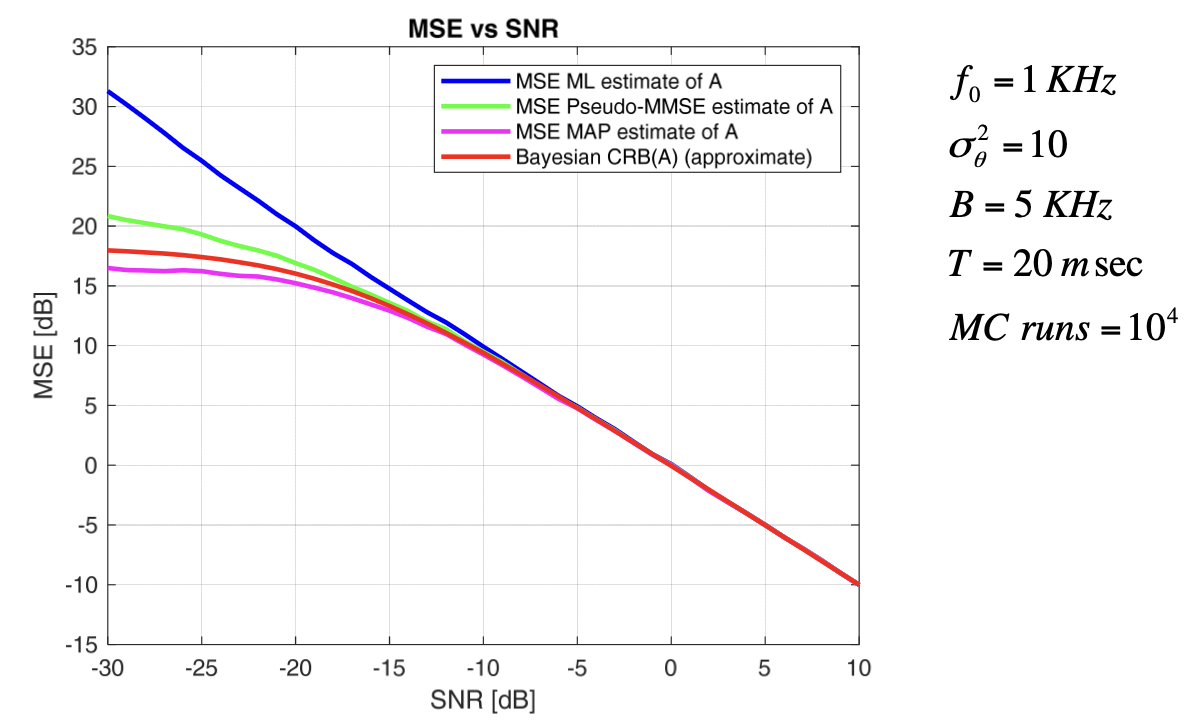
\includegraphics[width=0.65\linewidth]{Image/pdf 7/12.MSE_vs_SNR_2.png}
    \label{fig:placeholder}
\end{figure}
\subsection{MAP estimation of a constant Laplacian signal in AWGN}
\noindent \textbf{Problem}: find the MAP estimator of constant random signal S in AWGN.
\[
\underbrace{Y_i = S + W_i \quad i = 0, 1, 2, \cdots, N-1;}_{\text{Model of the observed data}},  \qquad \underbrace{S \in \mathcal{L}(\lambda)}_{\text{Random constant signal}}, \qquad\underbrace{W_i \in \mathcal{N}\left(0, \sigma_W^2\right), \quad \{W_i\}_{i=0}^{N-1} \text{ IID}}_{\text{Noise samples}}
\]
\item The difference with respect to the previous case, already analyzed, is that \underline{the constant random}\\ \noindent \underline{signal \(S\)} is not Gaussian distributed but it follows the \underline{\textbf{Laplace distribution}}, so the \textit{a-posteriori} is no more Gaussian.

\item In the \underline{Gaussian case}, the MMSE and MAP estimators coincide are given by:
\[\hat{S}_{MMSE} = \hat{S}_{MAP} = \alpha \hat{S}_{ML} + (1 - \alpha)\eta_S \quad \text{\textbf{{where:}}} \quad \hat{S}_{ML} \triangleq \underbrace{\frac{1}{N} \mathbf{1}^T \mathbf{Y}}_{\text{Sample Mean}}, \quad \alpha \triangleq \frac{N\gamma}{1 + N\gamma}, \quad \gamma \triangleq \frac{\sigma_S^2}{\sigma_W^2}\]
\item In this case, \underline{the MMSE and MAP estimators are different}, and it is not possible to find the MMSe estimator in closed form. Let us derive the \textbf{MAP estimator}.
\item The \textbf{MAP A Posteriori (MAP)} estimator are given by the \textbf{mode} of the \textit{a-posteriori} pdf :
\[
\hat{S}_{MAP}=\underset{s}{\arg\max} f_{S\mid\textbf{Y}}(s\mid\textbf{y})
\]
\item To maximize the \textit{a-posteriori} pdf w.r.t \(S\) is equivalent to maximize the joint pdf of the random parameter \(S\) and of the data vector \textbf{Y}:
\begin{align*}
&\hat{S}_{MAP} = \arg \max_s f_{S|\mathbf{Y}}(s|\mathbf{y}) = \arg \max_s \frac{f_{S,\mathbf{Y}}(s,\mathbf{y})}{f_{\mathbf{Y}}(\mathbf{y})} = \arg \max_s f_{S,\mathbf{Y}}(s,\mathbf{y}) \\[5pt]
&= \arg \max_s f_{\mathbf{Y}|S}(\mathbf{y}|s) f_S(s) \\[5pt]
&\text{MAP equation:}  \quad \frac{\partial}{\partial s} \left[ \ln f_{\mathbf{Y}|S}(\mathbf{y}|s) + \ln f_S(s) \right] \bigg|_{s=\hat{S}_{MAP}} = 0
\end{align*}



\item Lets find \(f_{\mathbf{Y\mid s}}({\mathbf{y}\mid s})\):
\begin{align*}
&f_S(s) = \frac{1}{2\lambda} e^{-\frac{|s|}{\lambda}} \quad \rightarrow \quad E\{S^2\} = 2\lambda^2 \quad \text{Laplace distribution} \\[8pt]
&f_{\mathbf{Y}|S}(\mathbf{y}|s) = \prod_{i=0}^{N-1} f_{Y_i|S}(y_i|s) = \prod_{i=0}^{N-1} \frac{1}{\sqrt{2\pi\sigma_W^2}} e^{-\frac{(y_i - s)^2}{2\sigma_W^2}} 
= \left( 2\pi\sigma_W^2 \right)^{-\frac{N}{2}} e^{-\frac{1}{2\sigma_W^2} \sum_{i=0}^{N-1} (y_i - s)^2} \\[8pt]
&\ln f_{\mathbf{Y}|S}(\mathbf{y}|s) + \ln f_S(s) = \kappa_1 - \frac{1}{2\sigma_W^2} \sum_{i=0}^{N-1} (y_i - s)^2 - \frac{|s|}{\lambda}
\end{align*}
\item Continuing the derivation:

\begin{align*}
\ln f_{\mathbf{Y}|S}(\mathbf{y}|s) &= \kappa_1 - \frac{1}{2\sigma_W^2} \sum_{i=0}^{N-1} (y_i - s)^2 \\[10pt]
&= \kappa_1 - \frac{1}{2\sigma_W^2} \sum_{i=0}^{N-1} (y_i^2 - 2y_i s + s^2) = \kappa_1 - \frac{1}{2\sigma_W^2} \sum_{i=0}^{N-1} y_i^2 + \frac{s}{\sigma_W^2} \sum_{i=0}^{N-1} y_i - \frac{N}{2\sigma_W^2} s^2 \\[10pt]
&= - \frac{N}{2\sigma_W^2} (s^2 - 2Y_{SM} s + \kappa_2) = - \frac{N}{2\sigma_W^2} (s - Y_{SM})^2 + \kappa_3 \\[10pt]
\text{where} \quad Y_{SM} &\triangleq \frac{1}{N} \sum_{i=0}^{N-1} Y_i = \frac{1}{N} \mathbf{1}^T \mathbf{Y} \quad \text{Sample Mean}
\end{align*}
\begin{figure}[H]
    \centering
    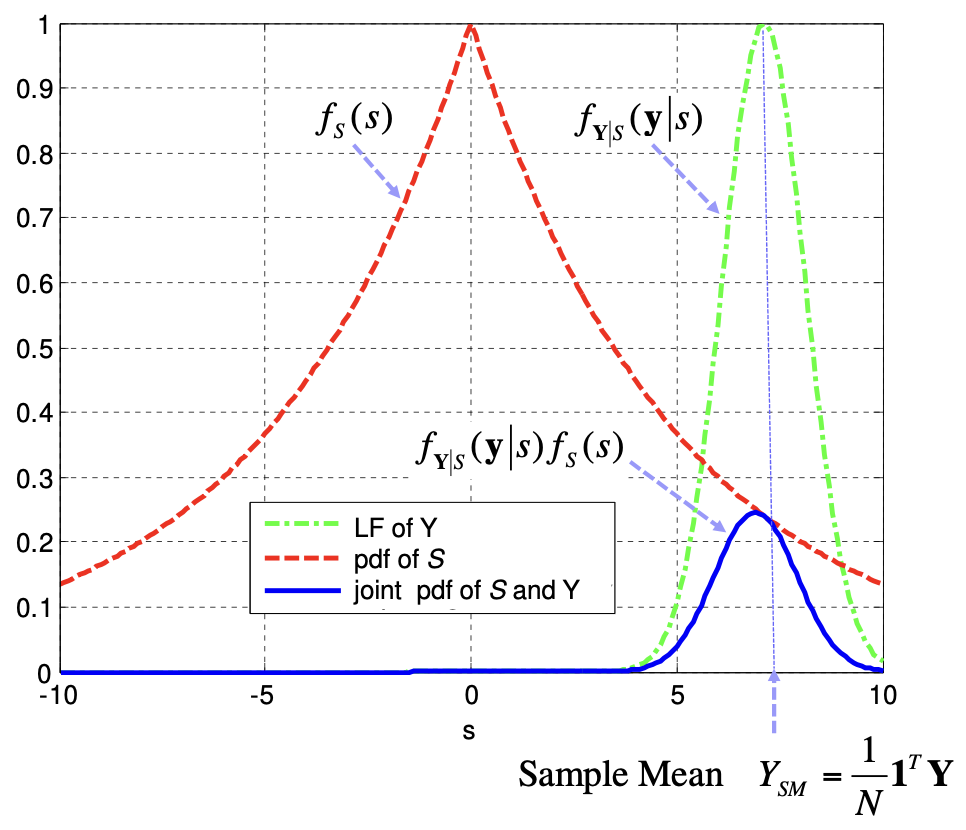
\includegraphics[width=0.55\linewidth]{Image/pdf 7/13.LF_pdf_joint.png}
    \label{fig:placeholder}
\end{figure}
\item Remind the formula:
\begin{align*}
\ln f_{\mathbf{Y}|S}(\mathbf{y}|s) + \ln f_S(s) &= - \frac{N}{2\sigma_W^2} (s - Y_{SM})^2 + \kappa_3 - \frac{|s|}{\lambda} \\[8pt]
&= - \frac{N}{2\sigma_W^2} \left( s^2 - 2Y_{SM} s + Y_{SM}^2 + \frac{2\sigma_W^2}{N} \frac{|s|}{\lambda} \right) + \kappa_3\\[8pt]
&= - \frac{N}{2\sigma_W^2} \left( s^2 + \frac{2\sigma_W^2}{N\lambda} |s| - 2Y_{SM} s + \kappa_4 \right)\\[8pt]
&\text{where} \quad Y_{SM} \triangleq \frac{1}{N} \sum_{i=0}^{N-1} Y_i = \frac{1}{N} \mathbf{1}^T \mathbf{Y} \quad \text{Sample Mean}\\[8pt]
\end{align*}\vspace{-1em}
\[\text{MAP equation}:\frac{\partial}{\partial s} \left[ \ln f_{\mathbf{Y}|S}(\mathbf{y}|s) + \ln f_S(s) \right] = \frac{\partial}{\partial s} \left( s^2 + \frac{2\sigma_W^2}{N\lambda} |s| - 2Y_{SM} s + \kappa_4 \right) = 0
\]
\item We can find the solution by differiating w.r.t \(s\) only if the maximum is at a value where the joint pdf is continuous, i.e. this case only if the solution is different from \(s=0\) (there is corner point at \(s=0\)):
\begin{align*}
&\frac{\partial}{\partial s} \left( s^2 + \frac{2\sigma_W^2}{N\lambda} |s| - 2Y_{SM} s + \kappa_4 \right) = 2s + \frac{2\sigma_W^2}{N\lambda} \text{sign}\{s\} - 2Y_{SM} = 0 \\[8pt]
s &= Y_{SM} - \frac{\sigma_W^2}{N\lambda} \text{sign}\{s\} \\[8pt]
&\begin{cases}
\hat{S}_{MAP} = Y_{SM} - \frac{\sigma_W^2}{N\lambda} \text{sign}\{\hat{S}_{MAP}\} = Y_{SM} - \frac{\sigma_W^2}{N\lambda} & \text{if } Y_{SM} - \frac{\sigma_W^2}{N\lambda} > 0 \\
\hat{S}_{MAP} = Y_{SM} - \frac{\sigma_W^2}{N\lambda} \text{sign}\{\hat{S}_{MAP}\} = Y_{SM} + \frac{\sigma_W^2}{N\lambda} & \text{if } Y_{SM} + \frac{\sigma_W^2}{N\lambda} < 0
\end{cases}
\end{align*}
\item In compact form, taking into account that \(\text{sign}\{\hat{S}_{MAP}\}=\text{sign}\{Y_{SM}\}\), we have :
\[
\hat{S}_{MAP}=Y_{SM}-\frac{\sigma_W^2}{N\lambda}\text{sign}\{Y_{SM}\}, \quad|Y_{SM}|>\frac{\sigma_W^2}{N\lambda}
\]
\item The MAP estimate is 0 otherwise:
$$\hat{S}_{MAP} = 0 \quad \text{if } \left| Y_{SM} \right| \leq \frac{\sigma_W^2}{N \lambda}
$$
$$
\text{sign} \left\{ \hat{S}_{MAP} \right\} = \text{sign} \left\{ Y_{SM} \right\} \quad \text{when } \hat{S}_{MAP} \neq 0
$$
\item \(s\geq 0\) case:
\begin{figure}[H]
    \centering
    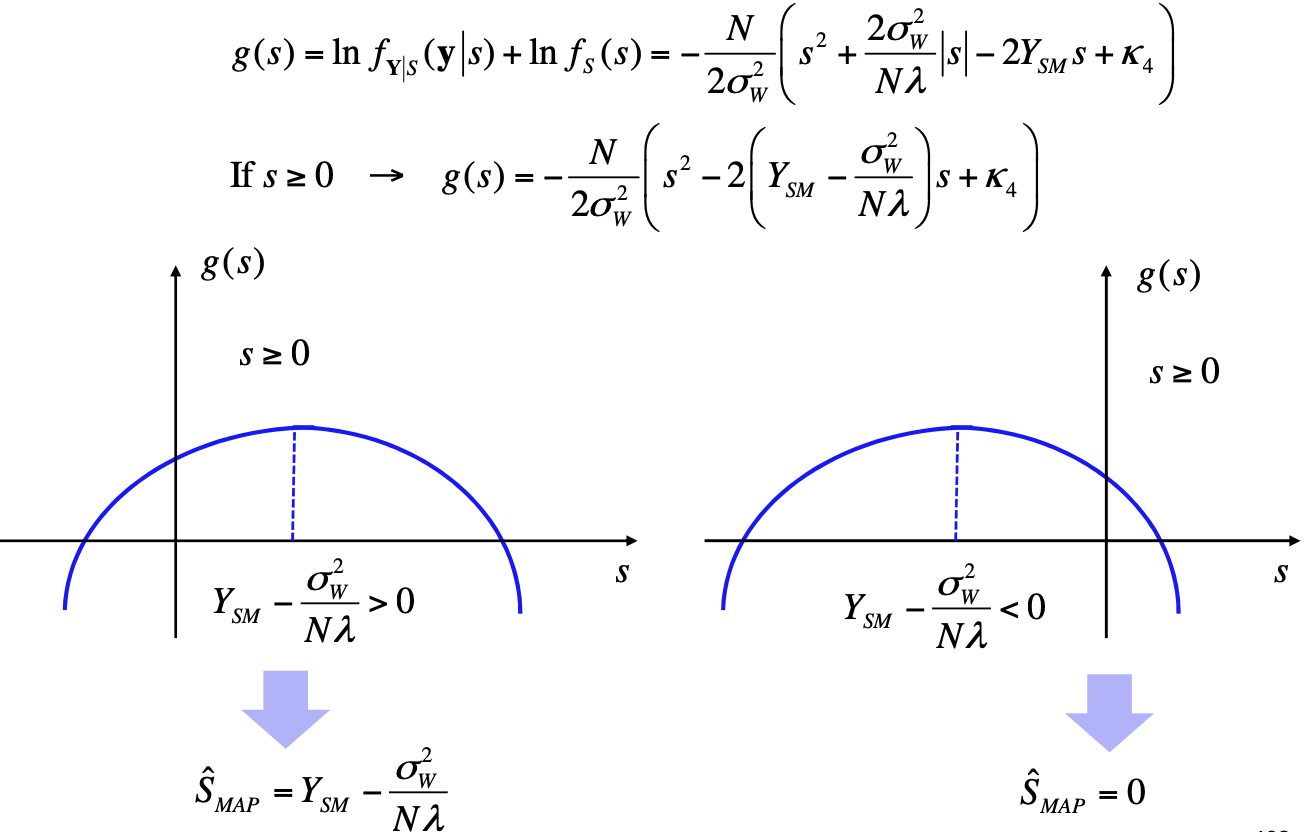
\includegraphics[width=0.55\linewidth]{Image/pdf 7/14.MAP_estime.png}
    \label{fig:placeholder}
\end{figure}
\item \(s\leq 0\) case:
\begin{figure}[H]
    \centering
    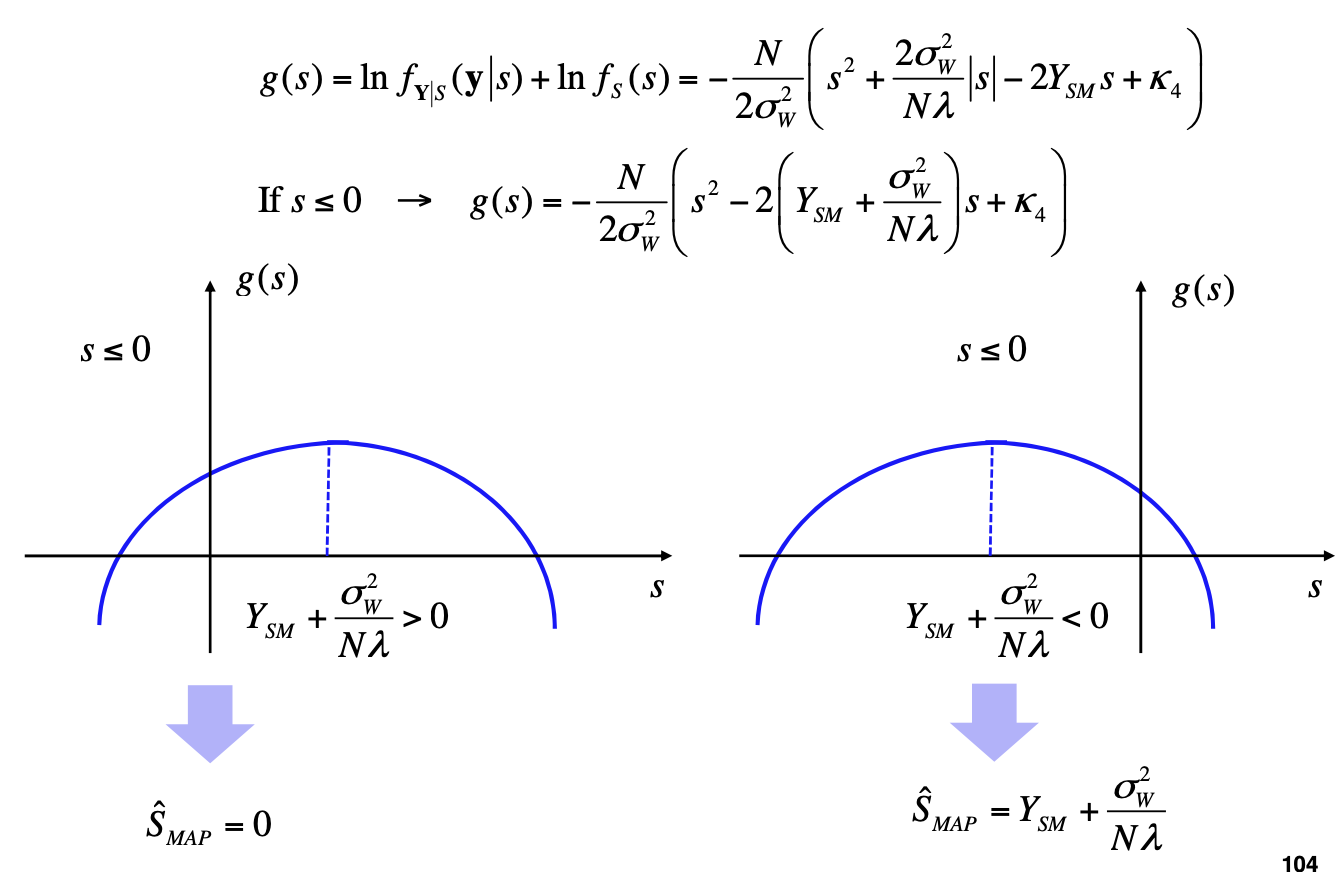
\includegraphics[width=0.55\linewidth]{Image/pdf 7/15.MAP_estime_s<0.png}
    \label{fig:placeholder}
\end{figure}



\item MAP estimate:
\begin{align*}
\hat{S}_{MAP} &= \begin{cases}
0, & \left| Y_{SM} \right| \leq \frac{\sigma_W^2}{N \lambda} \\
Y_{SM} - \frac{\sigma_W^2}{N \lambda} \text{sign}\left\{ Y_{SM} \right\}, & \left| Y_{SM} \right| > \frac{\sigma_W^2}{N \lambda}
\end{cases}
\end{align*}
\item ML estimate: \(\hat{S}_{ML}=Y_{SM}\)
\begin{figure}[H]
    \centering
    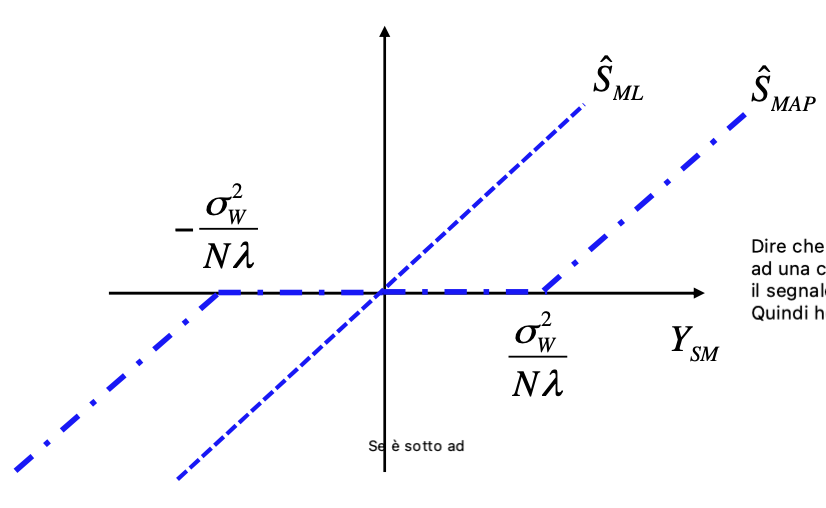
\includegraphics[width=0.55\linewidth]{Image/pdf 7/16.BO.png}
    \label{fig:placeholder}
\end{figure}

\item Some changes:

\[
SNR\triangleq\frac{E\{S^2\}}{E\{W_i^2\}}=\frac{2\lambda^2}{\sigma_W^2}\quad\rightarrow\quad\frac{\sigma_W^2}{N\lambda}=\frac{2\lambda}{N\cdot SNR}
\]
\begin{figure}[H]
    \centering
    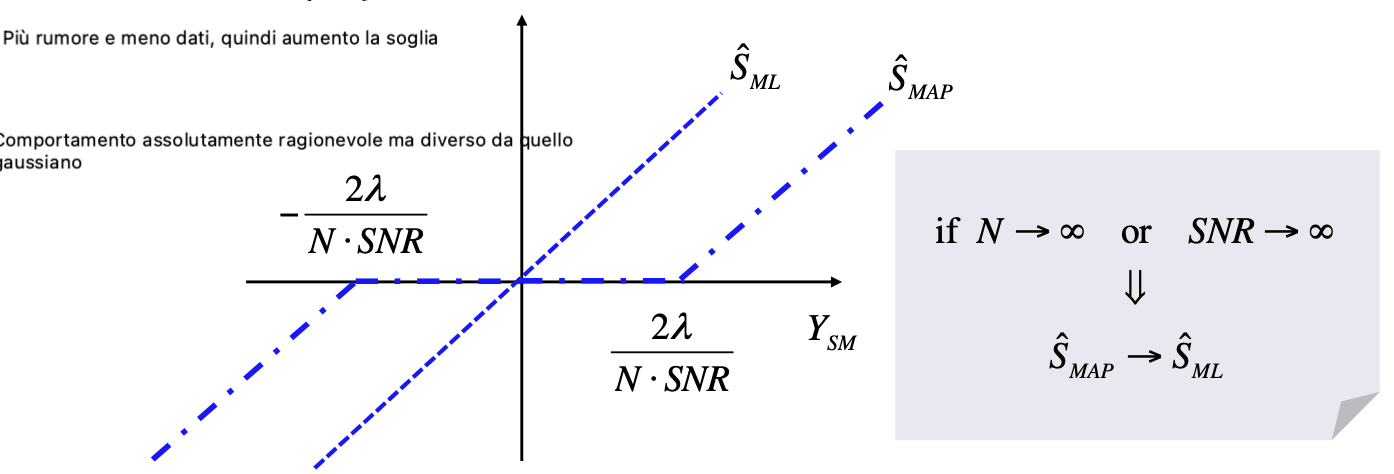
\includegraphics[width=0.55\linewidth]{Image/pdf 7/17.BO_2.png}
    \label{fig:placeholder}
\end{figure}
\item \textbf{MAP estimator} \(\rightarrow\) \textbf{Thresholding \& Denoising effect}: it uses the observed data, actually the sample mean of the data, only if its absolute value is greater than a given threshold, that is a function of the \textit{SNR} and of the data size \(N\). Otherwise, the estimate is given by the mode of the \textit{a-priori} pdf, which is 0.
\begin{align*}
&BCRB(S) = - \frac{1}{E_{S,\mathbf{Y}} \left\{ \frac{\partial^2 \ln f_{S,\mathbf{Y}}(s,\mathbf{y})}{\partial s^2} \right\}} \\[12pt]
&E_{S,\mathbf{Y}} \left\{ \frac{\partial^2 \ln f_{S,\mathbf{Y}}(s,\mathbf{y})}{\partial s^2} \right\} = E_{S,\mathbf{Y}} \left\{ \frac{\partial^2 \ln (f_{\mathbf{Y}|S}(\mathbf{y}|s)f_S(s))}{\partial s^2} \right\} = E_{S,\mathbf{Y}} \left\{ \frac{\partial^2 \ln f_{\mathbf{Y}|S}(\mathbf{y}|s)}{\partial s^2} + \frac{\partial^2 \ln f_S(s)}{\partial s^2} \right\} \\[12pt]
&= E_{S,\mathbf{Y}} \left\{ \frac{\partial^2 \ln f_{\mathbf{Y}|S}(\mathbf{y}|s)}{\partial s^2} \right\} + E_{S,\mathbf{Y}} \left\{ \frac{\partial^2 \ln f_S(s)}{\partial s^2} \right\} = E_S \left\{ E_{\mathbf{Y}|s} \left\{ \frac{\partial^2 \ln f_{\mathbf{Y}|S}(\mathbf{y}|s)}{\partial s^2} \right\} \right\} + E_S \left\{ \frac{\partial^2 \ln f_S(s)}{\partial s^2} \right\}
\end{align*}

\item Altre formule:

\begin{align*}
&\ln f_{\mathbf{Y}|S}(\mathbf{y}|s) = \ln \left( \frac{1}{(2\sigma_W^2)^{N/2}} \right) - \frac{1}{2\sigma_W^2} \sum_{i=0}^{N-1} (y_i - s)^2, \quad \ln f_S(s) = \ln \left( \frac{1}{2\lambda} \right) - \frac{|s|}{\lambda} \\[10pt]
&\begin{cases}
\frac{\partial \ln f_{\mathbf{Y}|S}(\mathbf{y}|s)}{\partial s} = \frac{1}{\sigma_W^2} \sum_{i=0}^{N-1} (y_i - s) = \frac{1}{\sigma_W^2} \sum_{i=0}^{N-1} y_i - \frac{N}{\sigma_W^2} s, & \frac{\partial^2 \ln f_{\mathbf{Y}|S}(\mathbf{y}|s)}{\partial s^2} = - \frac{N}{\sigma_W^2} \\[10pt]
\frac{\partial \ln f_S(s)}{\partial s} = - \frac{1}{\lambda} \text{sign}(s), & \frac{\partial^2 \ln f_S(s)}{\partial s^2} = - \frac{2}{\lambda} \delta(s)
\end{cases} \\[10pt]
&E_S \left\{ E_{\mathbf{Y}|s} \left\{ \frac{\partial^2 \ln f_{\mathbf{Y}|S}(\mathbf{y}|s)}{\partial s^2} \right\} \right\} = - \frac{N}{\sigma_W^2}
\end{align*}

\item And finally:

\begin{align*}
E_S \left\{ \frac{\partial^2 \ln f_S(s)}{\partial s^2} \right\} &= \int_{-\infty}^{+\infty} - \frac{2}{\lambda} \delta(s) f_S(s) ds = - \frac{2}{\lambda} \delta(s) f_S(0) = - \frac{2}{\lambda} \cdot \frac{1}{2\lambda} = - \frac{1}{\lambda^2} \\[10pt]
BCRB(S) &= - \frac{1}{E_{S,\mathbf{Y}} \left\{ \frac{\partial^2 \ln f_{S,\mathbf{Y}}(s,\mathbf{y})}{\partial s^2} \right\}} = \frac{1}{\frac{N}{\sigma_W^2} + \frac{1}{\lambda^2}} = \frac{\lambda^2}{1 + \frac{N\lambda^2}{\sigma_W^2}} \\[10pt]
&= \frac{\lambda^2}{1 + N \cdot SNR/2} \\[20pt]
\text{where:} \quad SNR &= \frac{2\lambda^2}{\sigma_W^2}
\end{align*}
\begin{figure}[H]
    \centering
    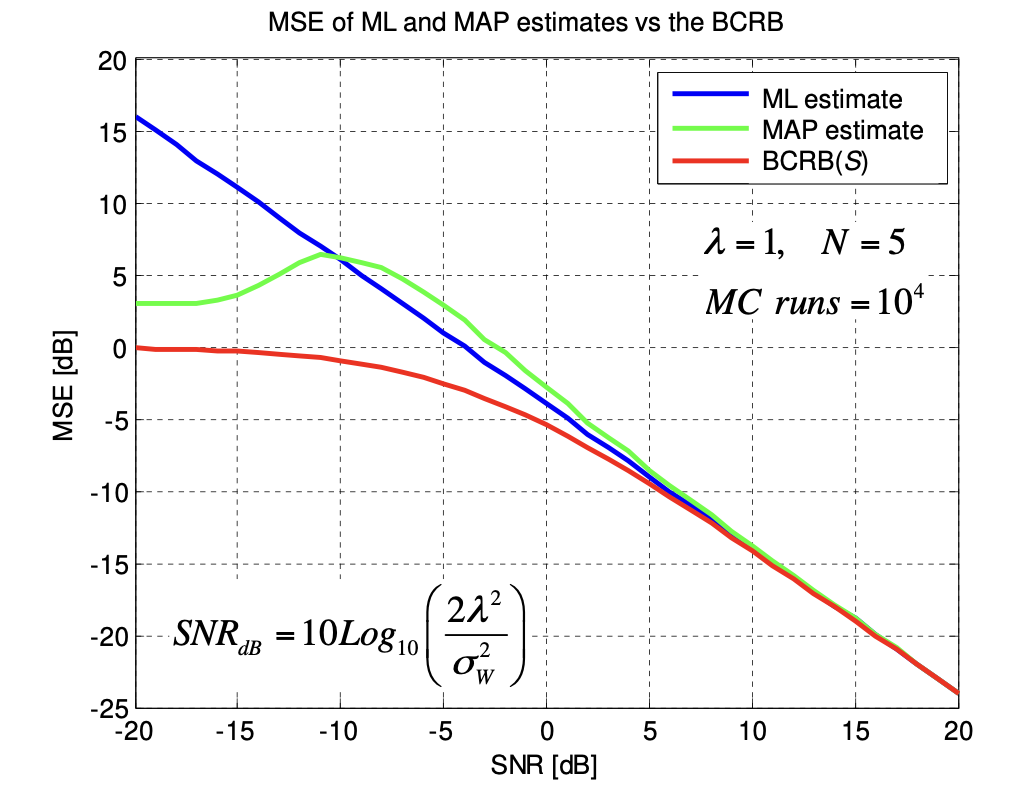
\includegraphics[width=0.55\linewidth]{Image/pdf 7/18.MSE of ML_1.png}
    \label{fig:placeholder}
\end{figure}
\begin{figure}[H]
    \centering
    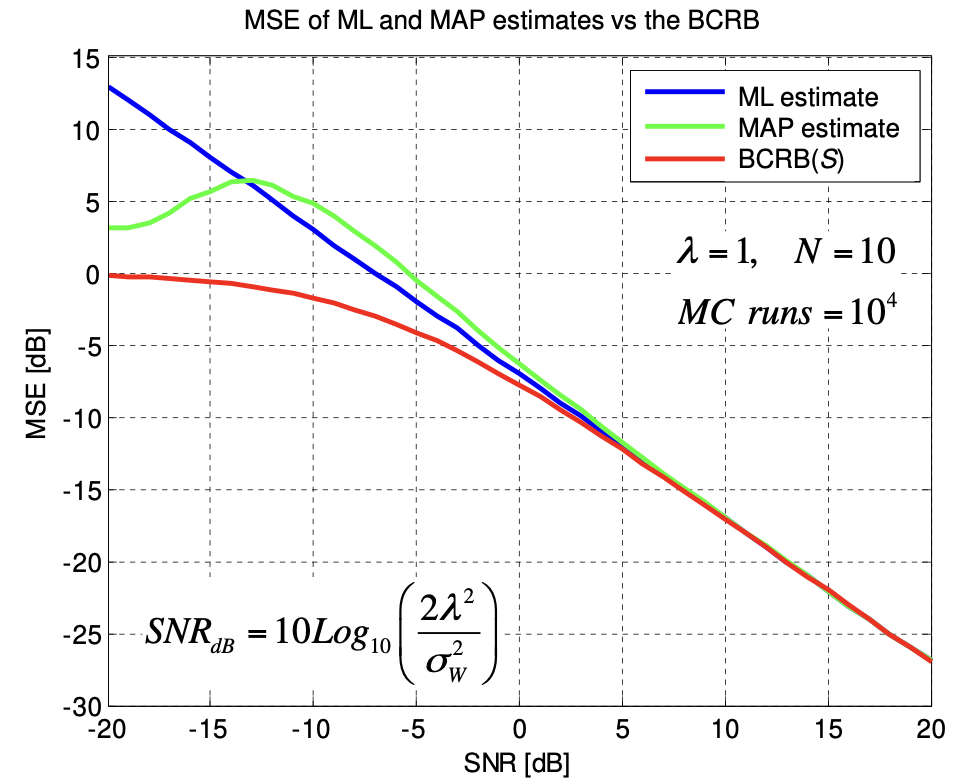
\includegraphics[width=0.55\linewidth]{Image/pdf 7/19.MSE_of_ML_2.png}
    \label{fig:placeholder}
\end{figure}
\begin{figure}[H]
    \centering
    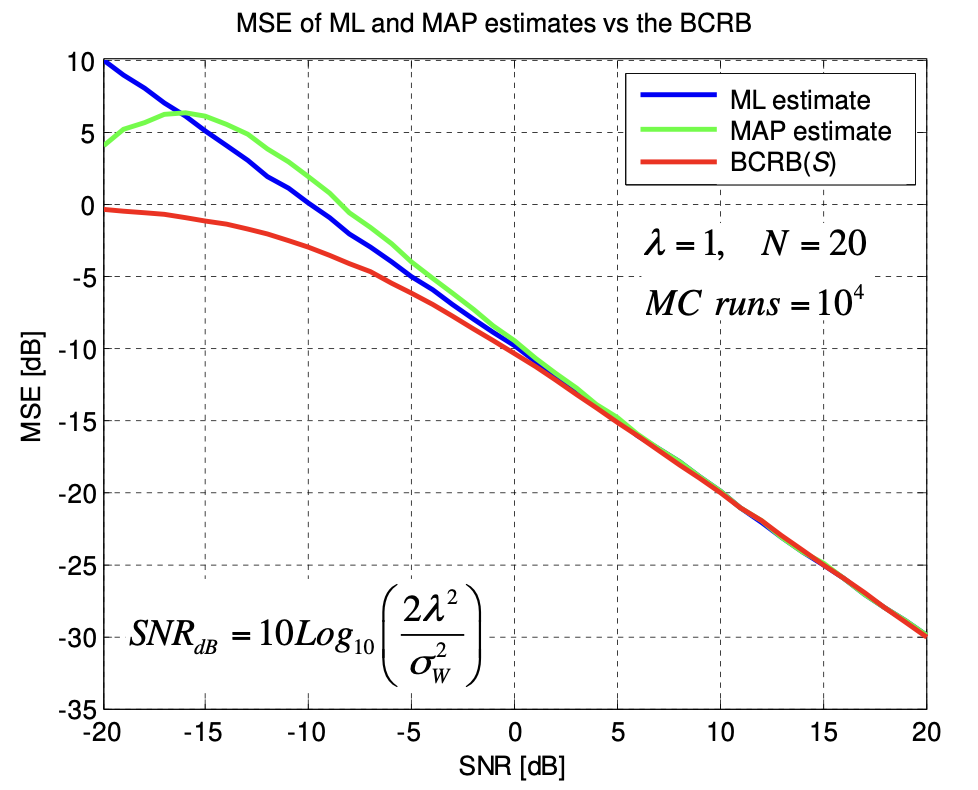
\includegraphics[width=0.55\linewidth]{Image/pdf 7/20.MSE_of_ML_3.png}
    \label{fig:placeholder}
\end{figure}
\begin{figure}[H]
    \centering
    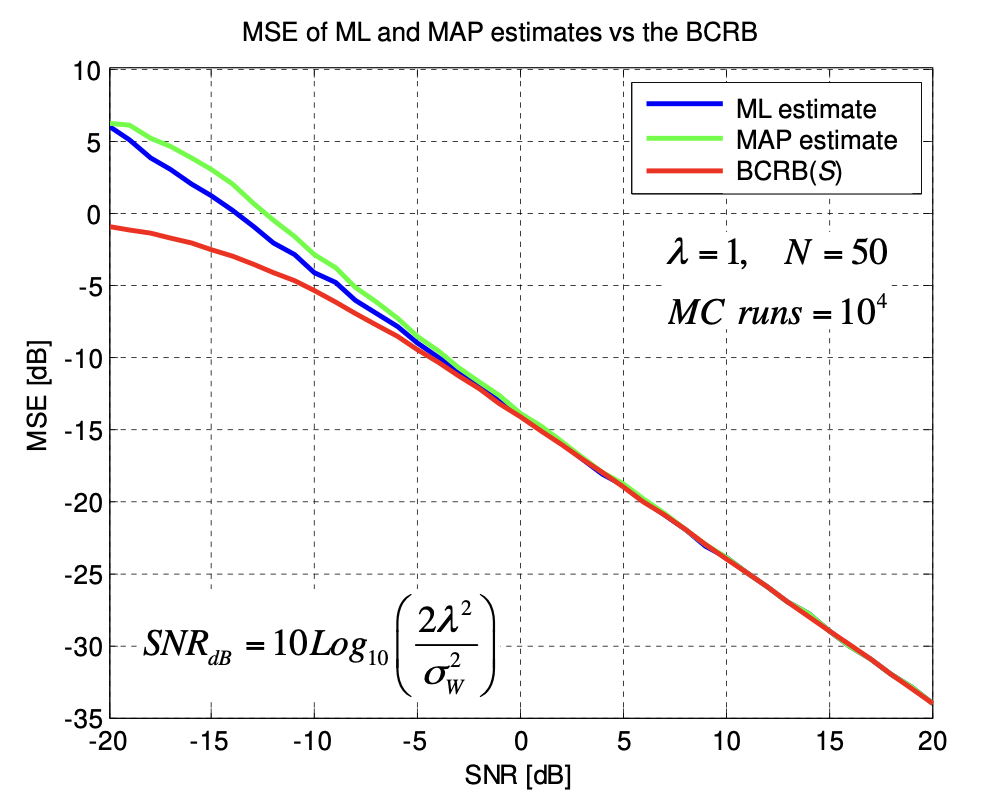
\includegraphics[width=0.55\linewidth]{Image/pdf 7/21.MSE_of_ML_4.png}
    \label{fig:placeholder}
\end{figure}
\begin{figure}[H]
    \centering
    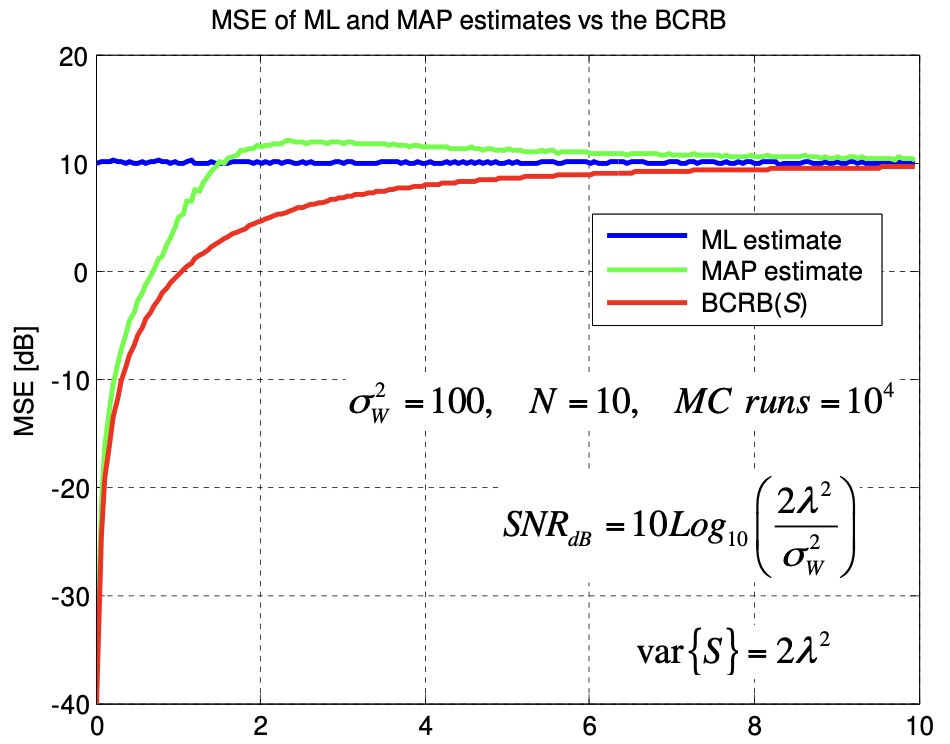
\includegraphics[width=0.55\linewidth]{Image/pdf 7/22.MSE_of_ML_5.png}
    \label{fig:placeholder}
\end{figure}
\begin{figure}[H]
    \centering
    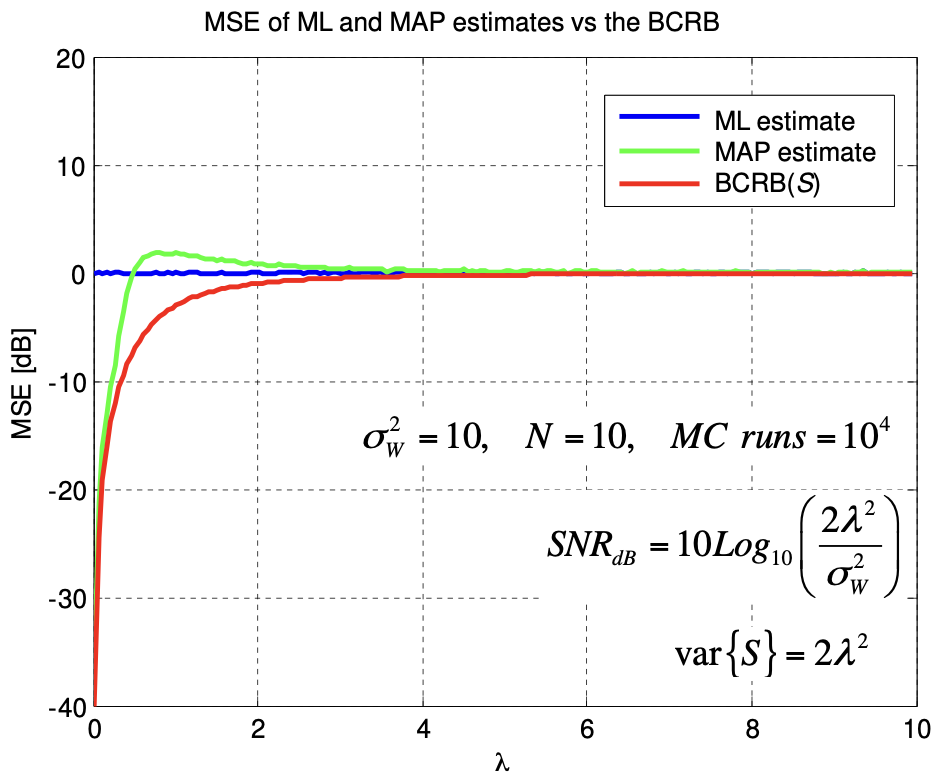
\includegraphics[width=0.55\linewidth]{Image/pdf 7/23.MSE_of_ML_6.png}
    \label{fig:placeholder}
\end{figure}
\begin{figure}[H]
    \centering
    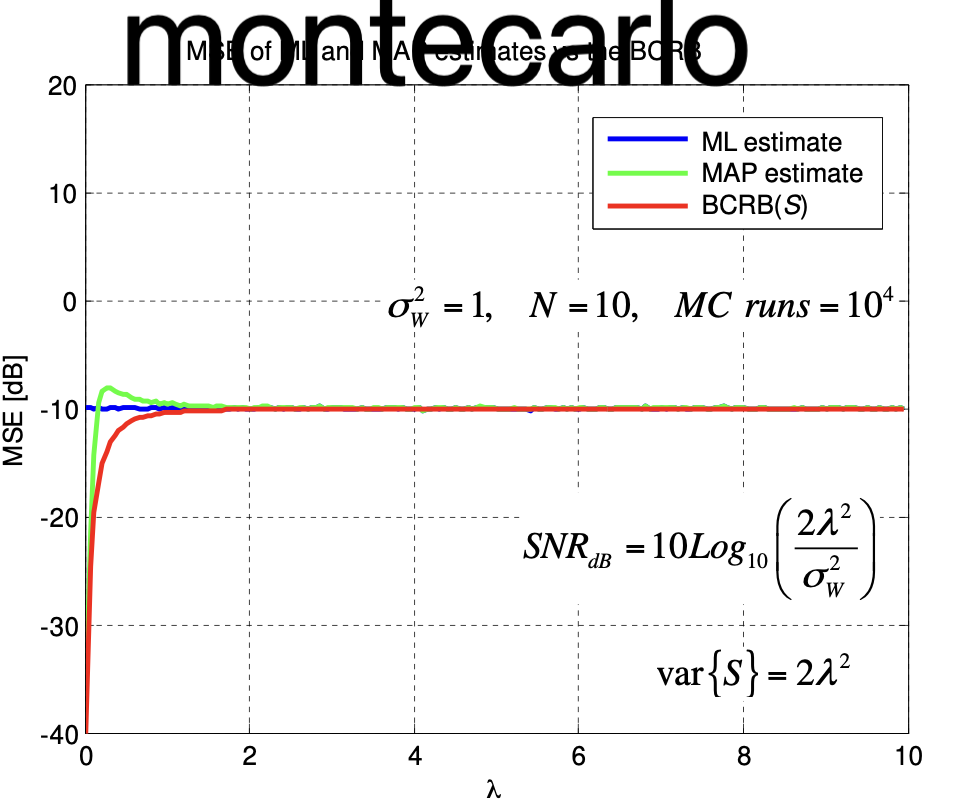
\includegraphics[width=0.55\linewidth]{Image/pdf 7/24.MSE_of_ML_7.png}
    \label{fig:placeholder}
\end{figure}
\end{itemize}
\subsubsection{MAP estimation of the parameter of an Exp distribution}
\noindent \textbf{Problem}: MAP estimation of the parameter \(\eta\) of an exponential distribution.
\begin{itemize}
    \item We observe \(N\) realizations of an exponentially distributed r.v. Y and we want to estimate the parameter \(\eta\) of the pdf under the assumption that the unknown parameter can be modelled as a r.v. with \textit{a-priori} pdf which is exponential with known parameter \(\lambda\). Conditionally to a given value of \(\eta\) the observed data are IID.
    \item Find the \textbf{MAP estimator} and compare it with the \textbf{ML estimator} of \(\eta\):

    \begin{align*}
& \text{Observed data: } \{ Y_i; i = 0, 1, 2, \cdots, N-1 \} \quad Y_i | \eta \in \mathcal{E}xp(\eta), \quad \text{IID}, \quad E\{Y_i|\eta\} = \frac{1}{\eta} \\[10pt]
& f_\eta(\eta) = \lambda e^{-\lambda \eta} u(\eta) \quad \rightarrow \quad E\{\eta\} = \frac{1}{\lambda}, \quad \sigma_\eta^2 = \text{var}\{\eta\} = \frac{1}{\lambda^2} \\[10pt]
& f_{\mathbf{Y}|\eta}(\mathbf{y}|\eta) = \prod_{i=0}^{N-1} f_{Y_i|\eta}(y_i|\eta) = \prod_{i=0}^{N-1} \eta e^{-\eta y_i} u(y_i) = \eta^N e^{-\eta \sum_{i=0}^{N-1} y_i} \prod_{i=0}^{N-1} u(y_i)
\end{align*}

\item The \textbf{Maximum Likelihood (ML)} estimator is given by the \textbf{mode} of the log-LF, i.e. the logarithm of the pdf of the observed data \textbf{Y} conditioned to a value of the unknown parameter \(\eta\):

\[
\hat{\eta}=\underset{\eta}{\arg\max}f_{\mathbf{Y}\mid\eta}(\mathbf{y}\mid\eta)
\]
\item If the log-LF is differentiable w.r.t \(\eta\), the ML estimate can be derived by solving the following equation:
$$
\text{ML equation:} \quad \frac{\partial \ln f_{\mathbf{Y}|\eta}(\mathbf{y}|\eta)}{\partial \eta} \bigg|_{\eta=\hat{\eta}_{ML}} = 0
$$
\vspace{-0.5em}
$$
\ln f_{\mathbf{Y}|\eta}(\mathbf{y}|\eta) = \ln \left( \eta^N e^{-\eta \sum_{i=0}^{N-1} y_i} \prod_{i=0}^{N-1} u(y_i) \right) = N \ln \eta - \eta \sum_{i=0}^{N-1} y_i
$$
\item Solving the ML equation we get:
\[
\frac{\partial}{\partial \eta} \left( N \ln \eta - \eta \sum_{i=0}^{N-1} y_i \right) = \frac{N}{\eta} - \sum_{i=0}^{N-1} y_i = 0 \quad \Rightarrow \quad \hat{\eta}_{ML} = \frac{N}{\sum_{i=0}^{N-1} y_i} = \frac{1}{\frac{1}{N} \sum_{i=0}^{N-1} y_i} = \frac{1}{Y_{SM}}
\]
\item The \textbf{Maximum A posteriori (MAP)} estimator is instead given by the \textbf{mode} of the a-posteriori pdf or equivalently by the value which maximizes the joint pdf of \textbf{Y} and \(\eta\):
$$
\hat{\eta}_{MAP} = \arg \max_{\eta} f_{\eta|\mathbf{Y}}(\eta|\mathbf{y}) = \arg \max_{\eta} f_{\mathbf{Y}|\eta}(\mathbf{y}|\eta) f_\eta(\eta)
$$
\vspace{-0.5em}
$$
MAP \text{ equation:} \quad \frac{\partial \left[ \ln f_{\mathbf{Y}|\eta}(\mathbf{y}|\eta) + \ln f_\eta(\eta) \right]}{\partial \eta} \bigg|_{\eta=\hat{\eta}_{MAP}} = 0
$$
\item To finish the derivation:

\begin{align*}
\frac{\partial \left[ \ln f_{\mathbf{Y}|\eta}(\mathbf{y}|\eta) + \ln f_\eta(\eta) \right]}{\partial \eta} &= \frac{N}{\eta} - \sum_{i=0}^{N-1} y_i + \frac{\partial \ln(\lambda e^{-\lambda \eta} u(\eta))}{\partial \eta} \\[10pt]
&= \frac{N}{\eta} - \sum_{i=0}^{N-1} y_i - \lambda = 0 \\[10pt]
\hat{\eta}_{MAP} = &\frac{N}{\sum_{i=0}^{N-1} y_i + \lambda} = \frac{1}{\frac{\lambda}{N} + \frac{1}{N} \sum_{i=0}^{N-1} y_i} \\[10pt]
= \frac{1}{Y_{SM} + \lambda/N}
\end{align*}
\item It is worth observing that when \(N\) tends to infinity (i.e. we have may data) or when \(\lambda\) tends to 0 (i.e. when the variance of the \textit{a-priori}) pdf tends to be very large, so that the \textit{a-priori} pdf is \textit{non-informative}, the MAP estimator tends to coincide with the ML estimator:
\[
\lim_{N\rightarrow+\infty}\hat{\eta}_{MAP} =\hat{\eta}_{ML}, \quad \lim_{\lambda\rightarrow0}\hat{\eta}_{MAP}=\hat{\eta}_{ML}
\]
\item Let us assume now that the data pdf is parametrized by \(\alpha = 1/\eta\) instead of \(\eta\):
\begin{align*}
&Y_i | \alpha \in \mathcal{E}xp(\alpha), \quad \text{IID}, \quad E\{Y_i|\alpha\} = \alpha \\[10pt]
&f_{\mathbf{Y}|\alpha}(\mathbf{y}|\alpha) = \prod_{i=0}^{N-1} f_{Y_i|\alpha}(y_i|\alpha) = \prod_{i=0}^{N-1} \frac{1}{\alpha} e^{-\frac{y_i}{\alpha}} u(y_i) = \left(\frac{1}{\alpha}\right)^N e^{-\frac{1}{\alpha}\sum_{i=0}^{N-1} y_i} \prod_{i=0}^{N-1} u(y_i) \\[10pt]
&f_\alpha(\alpha) = ? \quad \rightarrow \quad \alpha = g(\eta) = \frac{1}{\eta} \quad \rightarrow \quad f_\alpha(\alpha) = \frac{f_\eta(\eta)}{\left| \frac{d g(\eta)}{d \eta} \right|} \bigg|_{\eta=g^{-1}(\alpha)}
\end{align*}
\begin{align*}
f_\alpha(\alpha) &= \frac{f_\eta(\eta)}{\left| \frac{d g(\eta)}{d \eta} \right|} \bigg|_{\eta=g^{-1}(\alpha)} = \frac{\lambda e^{-\lambda \eta} u(\eta)}{\frac{1}{\eta^2}} \bigg|_{\eta=1/\alpha} = \frac{\lambda}{\alpha^2} e^{-\frac{\lambda}{\alpha}} u(\alpha) \\[10pt]
\ln f_{\mathbf{Y}|\alpha}(\mathbf{y}|\alpha) &= \ln \left[ \left(\frac{1}{\alpha}\right)^N e^{-\frac{1}{\alpha}\sum_{i=0}^{N-1} y_i} \prod_{i=0}^{N-1} u(y_i) \right] = -N \ln \alpha - \frac{1}{\alpha} \sum_{i=0}^{N-1} y_i \\[10pt]
\frac{\partial \ln f_{\mathbf{Y}|\alpha}(\mathbf{y}|\alpha)}{\partial \alpha} &= - \frac{N}{\alpha} + \frac{1}{\alpha^2} \sum_{i=0}^{N-1} y_i = 0 \quad \Rightarrow \quad \hat{\alpha}_{ML} = \frac{1}{N} \sum_{i=0}^{N-1} y_i = Y_{SM} = \frac{1}{\hat{\eta}_{ML}}
\end{align*}
\item \textbf{Invariancy property} of the ML estimate:
\[
\alpha=\frac{1}{\eta}\quad\Rightarrow\quad\hat{\alpha}_{ML}=\frac{1}{\hat{\eta}_{ML}}
\]
\item For the MAP estimate the invariance property holds only for affine transformations, but not for nonlinear transformations:
\[
\alpha=\frac{1}{\eta}\quad \nRightarrow \quad\hat{\alpha}_{MAP}=\frac{1}{\hat{\eta}_{MAP}}
\]
\item Let us derive the MAP estimator of \(\alpha\):
\begin{align*}
\ln f_{\mathbf{Y}|\alpha}(\mathbf{y}|\alpha) + \ln f_\alpha(\alpha) &= -N \ln \alpha - \frac{1}{\alpha} \sum_{i=0}^{N-1} y_i + \ln \left( \frac{\lambda}{\alpha^2} e^{-\frac{\lambda}{\alpha}} u(\alpha) \right)\\[8pt]
&= -N \ln \alpha - \frac{N}{\alpha} Y_{SM} + \ln \lambda - 2 \ln \alpha - \frac{\lambda}{\alpha}
\end{align*}
\item Differentiating w.r.t \(\alpha\) and solving the MAP equation we get:
\begin{align*}
\frac{\partial}{\partial \alpha} \left( \ln f_{\mathbf{Y}|\alpha}(\mathbf{y}|\alpha) + \ln f_\alpha(\alpha) \right) &= \frac{\partial}{\partial \alpha} \left( -N \ln \alpha - \frac{N}{\alpha} Y_{SM} + \ln \lambda - 2 \ln \alpha - \frac{\lambda}{\alpha} \right) \\[10pt]
&= - \frac{N}{\alpha} + \frac{N}{\alpha^2} Y_{SM} - \frac{2}{\alpha} + \frac{\lambda}{\alpha^2} = \frac{N Y_{SM} + \lambda - (N + 2)\alpha}{\alpha^2} = 0 \\[10pt]
\hat{\alpha}_{MAP} &= \frac{N Y_{SM} + \lambda}{N + 2} = \frac{Y_{SM} + \lambda/N}{1 + 2/N} \neq \frac{1}{\hat{\eta}_{MAP}}
\end{align*}
\item However, when \(N\) tends to infinity, the MAP estimator tends to coincide with the ML estimator, so the \textit{a-priori} information is less and less useful when the data size increases:

\begin{align*}
N \gg 1 \quad &\rightarrow \quad \hat{\eta}_{MAP} = \frac{1}{Y_{SM} + \lambda/N} \approx \frac{1}{Y_{SM}} = \hat{\eta}_{ML} \\[15pt]
N \gg 1 \quad &\rightarrow \quad \hat{\alpha}_{MAP} = \frac{Y_{SM} + \lambda/N}{1 + 2/N} \approx Y_{SM} = \hat{\alpha}_{ML}
\end{align*}
\item This results holds true in general: \underline{when the sample size \(N\) tends to infinty, the MAP estimator tends}\\ \noindent \underline{to coincide with the ML estimator, which does not use the \textit{a-priori} information}.
\item Let us now drive the BCRB for the random parameter \(\eta\):
\begin{align*}
BCRB(\eta) &= - \frac{1}{E_{\eta,\mathbf{Y}} \left\{ \frac{\partial^2 \ln f_{\eta,\mathbf{Y}}(\eta,\mathbf{y})}{\partial \eta^2} \right\}} \\[15pt]
&E_{\eta,\mathbf{Y}} \left\{ \frac{\partial^2 \ln f_{\eta,\mathbf{Y}}(\eta,\mathbf{y})}{\partial \eta^2} \right\} = E_{\eta,\mathbf{Y}} \left\{ \frac{\partial^2 \ln (f_{\mathbf{Y}|\eta}(\mathbf{y}|\eta)f_\eta(\eta))}{\partial \eta^2} \right\} \\[15pt]
&= E_{\eta,\mathbf{Y}} \left\{ \frac{\partial^2 \ln f_{\mathbf{Y}|\eta}(\mathbf{y}|\eta)}{\partial \eta^2} + \frac{\partial^2 \ln f_\eta(\eta)}{\partial \eta^2} \right\} \\[10pt]
&= E_{\eta,\mathbf{Y}} \left\{ \frac{\partial^2 \ln f_{\mathbf{Y}|\eta}(\mathbf{y}|\eta)}{\partial \eta^2} \right\} + E_{\eta,\mathbf{Y}} \left\{ \frac{\partial^2 \ln f_\eta(\eta)}{\partial \eta^2} \right\} \\[10pt]
&= E_{\eta} \left\{ E_{\mathbf{Y}|\eta} \left\{ \frac{\partial^2 \ln f_{\mathbf{Y}|\eta}(\mathbf{y}|\eta)}{\partial \eta^2} \right\} \right\} + E_{\eta} \left\{ \frac{\partial^2 \ln f_\eta(\eta)}{\partial \eta^2} \right\}
\end{align*}
\item Continuing the derivation:
\begin{align*}
&\frac{\partial \ln f_{\mathbf{Y}|\eta}(\mathbf{y}|\eta)}{\partial \eta} + \frac{\partial \ln f_\eta(\eta)}{\partial \eta} = \frac{N}{\eta} - \sum_{i=1}^{N} y_i - \lambda \\[10pt]
&\frac{\partial^2 \ln f_{\mathbf{Y}|\eta}(\mathbf{y}|\eta)}{\partial \eta^2} + \frac{\partial^2 \ln f_\eta(\eta)}{\partial \eta^2} = - \frac{N}{\eta^2} \qquad E_{\eta,\mathbf{Y}} \left\{ \frac{\partial^2 \ln f_{\eta,\mathbf{Y}}(\eta,\mathbf{y})}{\partial \eta^2} \right\} = -N \cdot E_\eta \left\{ \frac{1}{\eta^2} \right\}
\end{align*}
\item We obtain:
\[
\boxed{MSE\{\hat{\eta}\} \geq BCRB(\eta) = \frac{1}{N \cdot E\{1/\eta^2\}} \leq \frac{1}{N} E\{\eta^2\} = \frac{2}{N\lambda^2} = ACRB(\eta)}
\]
\vspace{-0.5em}
\[
E \left[ \Phi(\eta^2) \right] \geq \Phi \left( E\{\eta^2\} \right) \quad \text{due to the Jensen's inequality and the convexity of } \Phi(x) = \frac{1}{x}
\]
\item If \(\eta\) is deterministic:
\[
\frac{\partial^2 \ln f_{\mathbf{Y}|\eta}(\mathbf{y}|\eta)}{\partial \eta^2} = - \frac{N}{\eta^2} \quad \rightarrow \quad CRB(\eta) = - \frac{1}{E_{\mathbf{Y}} \left\{ \frac{\partial^2 \ln f_{\mathbf{Y}|\eta}(\mathbf{y}|\eta)}{\partial \eta^2} \right\}} = \frac{\eta^2}{N}
\]
\item The "average" CRB (ACRB) is given by:
\[
ACRB(\eta) = E_{\eta}\{CRB(\eta)\} = E_{\eta} \left\{ \frac{\eta^2}{N} \right\} = \frac{E_{\eta}\{\eta^2\}}{N} = \frac{2}{N\lambda^2}
\]
\item However, we cannot say that \(MSE\{\hat{\eta}\}\geq ACRB(\eta)\) is always valid. [it can proved that it is true only under some particular conditions]
\begin{figure}[H]
    \centering
    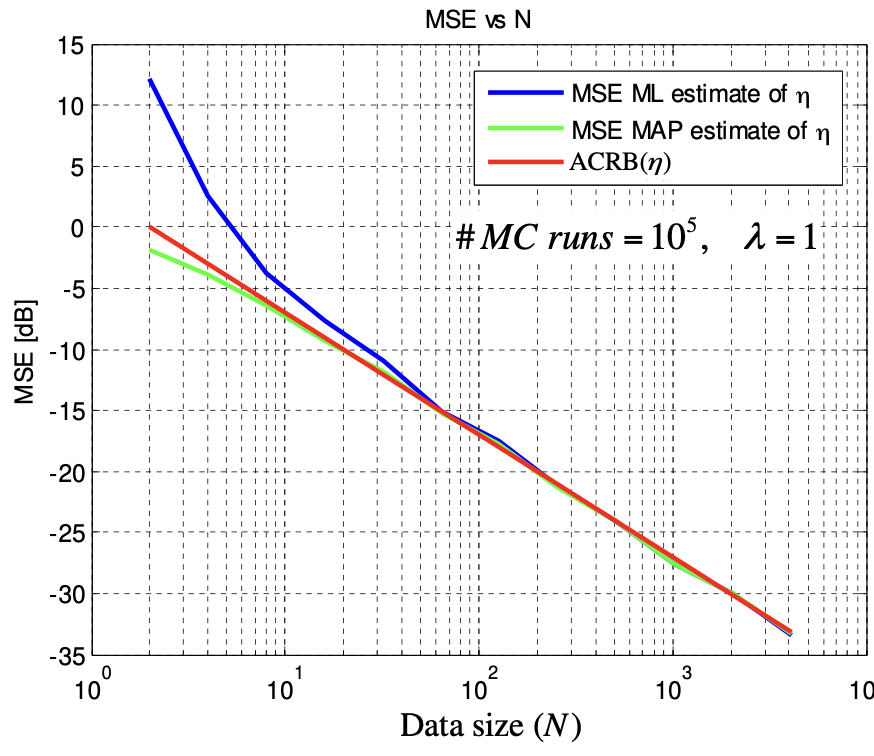
\includegraphics[width=0.65\linewidth]{Image/pdf 7/25.MAP_EXP.png}
    \label{fig:placeholder}
\end{figure}
\end{itemize}

\clearpage